%%%%%%%%%%%%%%%%%%%%%%%%%%%%%%%%%
%% usmthesis.cls 2016/12/08 version V1.7.
%%
%% IMPORTANT MESSAGE (Dec 2016)
%% Due to the recent numerous changes requested by IPS, USM to different
%% candidates -- often conflicting even within the same week -- without much
%% consistency nor in black in white, I have found it increasingly difficult
%% to maintain a coherent version. I have therefore decided to provide some
%% options that seem to be favored by IPS on different occasions; but will no
%% longer update the template until an updated formatting guidelines with clear
%% instructions and concrete samples is published.
%%
%% THERE WILL BE NO FURTHER UPDATES UNTIL IPS-USM PUBLISHES AN OFFICIAL
%% UPDATED FORMATTING GUIDELINES WITH CONCRETE, CLEAR INSTRUCTIONS.
%%
%% Individual requests for help to modify this version for your needs will be
%% handled on a case by case basis, depending on my mood, perhaps for a fee.
%% Requests for help to modify past versions will NOT be entertained.
%% Please read http://tex.my/how-to-ask-for-latex-related-help-effectively/.
%%
%% (Yes I'm that tired and frustrated. I know everyone just want to graduate,
%% but I am by now genuinely put off by the tone of some requests with rude
%% attitudes, unclear descriptions, flip-flopping conditions, etc for something
%% that was originally for my own use.)
%%
%% Usmthesis _was_ fun; but it has ceased to be so for me.
%%
%% Submit a git pull request on https://github.com/liantze/usmthesis
%% if you wish to contribute your changes. No timeframe is set for approvals.
%% I cannot check through any edited usmthesis.cls of any version without
%% CVS.
%%
%% Oh and if you'd like to adapt this template (the .cls and/or the .tex) for
%% your institution, that's perfectly fine, but at least keep the license
%% (LPPL 1.3) and the original author (me) won't you? It's just normal decency.
%% THANK you. :-)
%%%%%%%%%%%%%%%%%%%%%%%%%%%%%%%%%

%% If you prefer -- and have been allowed -- to use
%% Arial, then
%% \documentclass[arial]{usmthesis}
%% It's not really Arial, it's a Helvetica look-alike,
%% but if you're not a designer nor a typographer, you
%% probably can't tell the difference (I can't either)
%%
%% OTHER IMPORTANT OPTIONS:
%% singespacetitle - Make title on cover and title
%%                   page single-spaced.
%%
%% chapnumwords — Make chapter titles be `Chapter One'
%% tocchapnumwords — Make the ToC use `Chaper One' too
%%   (Engineering IPS seems to like the above two settings)
%%
%% tocpage   These options will add a ``Page'' label at the
%% lotpage   top of the Table of Contents, List of Tables,
%% lofpage   List of Figures and List of Plates respectively.
%% loppage   I don't know lah, one moment IPS says must add at
%%           the top of all these lists; one month later say
%%           only the ToC, a few months later say don't add at all.
%%           Find, mix-and-match yourself based on the instrustions you got.
%%
%% tocCAPSfront - Sometimes IPS wants the ``Table of Contents'', ``List of
%%                Figures'', ``Abstract'' etc to be all-caps in the ToC;
%%                sometimes they don't. Use this option to make them ALL CAPS.
%%
%% tocCAPSref - Similar to the above but for the ``References''.
%% tocCAPSapp - Similar to the above but for the ``Appendices''.
\documentclass[
singlespacetitle, % Make title on cover page singlespaced
% chapnumwords,tocchapnumwords,  %% ``Chapter One'' I think Engineering like this
tocpage,  % Put ``Page'' at top of ToC. Add lotpage, lofpage if
          % ``Page'' is also needed for LoT and LoF.
% tocCAPSfront, % Make ``List of Tables'' etc in ToC CAPS
% tocCAPSref, % Make ``References'' in ToC CAPS
% tocCAPSapp, % Make ``Appendices'' in ToC CAPS
]{usmthesis}

%%%%%%%%%%%%%%%%%%%%%%%%%%%%%%%%%%%%%%%%%%%%%%%%%%%%%%%
% This is usmthesis.tex, 6 Dec 2016. READ THE COMMENTS.
% Some formattings are easiest changed by uncommenting
% some lines in this .tex file or by changing certain
% options.
%
% Created by Lim Lian Tze (Ph.D.)
% liantze@gmail.com
% http://liantze.penguinattack.org.
%%%%%%%%%%%%%%%%%%%%%%%%%%%%%%%%%%%%%%%%%%%%%%%%%%%%%%%

\usepackage{pdfpages}
\usepackage{afterpage}
% \usepackage{import}

% Set font size to 13pt
\usepackage{scrextend}
\changefontsizes{13pt}

%% Example of loading other packages that you may require.
%% I'm loading the marvosym package so that I can produce a
%% smiley face with the command \Smiley.
\usepackage{marvosym}

%% Also, the enumitem package is great for customising
%% list environments.
\usepackage{enumitem}
\usepackage{tabu}
\usepackage{booktabs}
\usepackage{calligra}
\usepackage{multirow}
\usepackage{multicol}
\usepackage{bm}
\usepackage{bibentry}
\usepackage[super]{nth}

%% Listings is a nice package for typesetting code
%% listings. Other possible packages include fancyvrb,
%% minted, etc.
\usepackage{listings}
\lstset{basicstyle=\ttfamily,breaklines=true}

%% For those who need to produce algorithms and pseudocode.
%% There are a number of different packages available, but
%% unfortunately they tend not to work well together!
%% I'm using algorithmicx, specifically algpseucode, here.
\usepackage[chapter]{algorithm}
\usepackage{algpseudocode}
% \usepackage{algorithm, algorithmic}
% \usepackage{algorithm}
\usepackage{mathtools}
\usepackage{indentfirst}
\renewcommand{\thealgorithm}{\arabic{chapter}.\arabic{algorithm}} 

%% PHAT PLACE
\usepackage{caption}
\usepackage{graphicx}
\usepackage{subfig}
% \usepackage[font = footnotesize]{subcaption}
% \usepackage{subcaption} ERROR ?
\captionsetup[subfigure]{font=scriptsize,labelfont=scriptsize}
\captionsetup{compatibility=false}
\usepackage{ulem}
\usepackage{xcolor}
\usepackage[ruled,vlined, algo2e]{algorithm2e}
\usepackage{tcolorbox}
\usepackage{ulem}

\definecolor{commentcolor}{RGB}{110,154,155}   % define comment color
\newcommand{\PyComment}[1]{\ttfamily\textcolor{commentcolor}{\# #1}}  % add a "#" before the input text "#1"
\newcommand{\PyCode}[1]{\ttfamily\textcolor{black}{#1}} % \ttfamily is the code font
\usepackage{tcolorbox}
\tcbuselibrary{minted}
\usepackage{blindtext}
\usepackage{multicol}

\renewcommand{\comment}[1]{\textcolor{blue}{#1}}
% \usepackage{bibunits}
%------------------------------

%% Enter particulars about your thesis HERE
% Your Name
\author{
NGUYỄN NGỌC KHÔI NGUYÊN \hspace{1em} 19120106 \\
PHAN NGUYỄN THANH TÙNG  \hspace{1.8em} 19120424
}

% English title of your thesis
% \title{Medical Diagnosis with Deep Learning}
\title{Deep Fashion with \\ Outfit Recommendation and Try-on}
% Year submitted
\submityear{2023}
% Month submitted
\submitmonth{July}
%% Choose only 1 degree type! :-)
\degreetype{BACHELOR OF SCIENCE IN COMPUTER SCIENCE}
% \degreetype{Master of Science}
\lecturer{DR. LÊ TRUNG NGHĨA \\ ASSOC. PROF. TRẦN MINH TRIẾT}

%%%%%%%%%%%%%%%%%%%%%%%%%%%%%%%%%%%%%%%%%%%%%%%%%%%%%%%
% You can comment out the following line if you don't have a
% "List of Own Publications". And make it all caps yourself
% if it needs to be all caps in the ToC.
%%%%%%%%%%%%%%%%%%%%%%%%%%%%%%%%%%%%%%%%%%%%%%%%%%%%%%%
\newcites{own}{List of Publications}

\usepackage{ragged2e}
\usepackage{tikz}
\usepackage{multido}
\usetikzlibrary{calc}
\usepackage{longtable}
\usepackage{makecell}
% \usepackage{biblatex}
\usepackage{url}
\def\UrlBreaks{\do\/\do-}

%%%%%%%%%%%%%%%%%%%%%%%%%%%%%%%%%%%%%%%%%%%%%%%%%%%%%%%
% Options for generating hyperlinks when using pdfLaTeX
% This will cause the Table of Contents "Page" problem
%%%%%%%%%%%%%%%%%%%%%%%%%%%%%%%%%%%%%%%%%%%%%%%%%%%%%%%
\usepackage{hyperref}
\hypersetup{
    colorlinks=,
    citecolor=black,
    filecolor=black,
    linkcolor=black,
    urlcolor=black
}

\ifpdf
  \makeatletter
  \hypersetup{hypertexnames=false,
  pdfauthor={@author},pdftitle={@title}}
  \makeatother
\fi

\usepackage[numbers]{natbib}
\setlength{\bibsep}{10pt plus 0.3ex}
\bibliographystyle{unsrt}

\begin{document}
%%%%%%%%%%%%%%%%%%%%%%%%%%%%%%%%%%%%%%%%%%%%%%%%%%%%%%%
% Default bibliography style is apa (using
% \RequirePackage[natbibapa]{apacite} in the class file).
%
% If you prefer the number system though, use bibliography
% style "plainnat" for [1][2][3] or "alpha" for [Jon94] (the label
% will be auto-generated).
%%%%%%%%%%%%%%%%%%%%%%%%%%%%%%%%%%%%%%%%%%%%%%%%%%%%%%%
% \bibliographystyle{apacite}
% \bibliographystyleown{apacite}
% \bibliographystyle{plainnat}
% \bibliographystyleown{plainnat}
% \frontmatter
\renewcommand\bibname{\protect\leftline{References}}
%%%%%%%%%%%%%%%%%%%%%%%%%%%%%%%%%%%%%%%%%%%%%%%%%%%%%%%
% Inserts the cover page (the hard cover with gold-lettering)
% and the title page
%%%%%%%%%%%%%%%%%%%%%%%%%%%%%%%%%%%%%%%%%%%%%%%%%%%%%%%
\makecover


%%%%%%%%%%%%%%%%%%%%%%%%%%%%%%%%%%%%%%%%%%%%%%%%%%%%%%%
% MAKE SURE YOU HAVE A acknowledgements.tex FILE
%%%%%%%%%%%%%%%%%%%%%%%%%%%%%%%%%%%%%%%%%%%%%%%%%%%%%%%

\frontmatter
\chapter*{COMMENT OF THESIS'S ADVISOR}
\begin{tikzpicture}[remember picture, overlay]
  \draw[line width = 1pt] ($(current page.north west) + (1.2in,-1in)$) rectangle ($(current page.south east) + (-0.7in,1in)$);

\end{tikzpicture}
\multido{}{15}{\noindent\makebox[\linewidth]{\dotfill}\endgraf}
%Tp HCM, ngày .... tháng .... năm 2021\\
%Giáo viên hướng dẫn\\
\chapter{Acknowledgements}
\label{thanks}
% \setcounter{page}{1}
First and foremost, we would like to extend our heartfelt appreciation to our advisors, Dr. Le Trung Nghia and Assoc. Prof. Tran Minh Triet, for their invaluable guidance and unwavering support throughout the completion of this thesis. Their expertise, constant encouragement, constructive feedback and inspirational motivation have played a pivotal role in moulding the progress of this thesis. We are deeply grateful for their helpful advice, which not only helps us in this thesis but also in terms of professional work ethic and attitude.

Secondly, we want to express our gratitude to the Faculty of Information Technology members at the University of Science, VNU-HCM. Their knowledge and guidance have profoundly influenced our academic journey and fostered a strong foundation for us to carry out this research. 
% The valuable lessons, suggestions, and discussions provided by these esteemed individuals have significantly enhanced our understanding of the topic and enriched the quality of our work.

We are also indebted to our teachers and friends at SELAB and Honors Program Class 19, Faculty of Information Technology at the University of Science, VNU-HCM, for their support, advice, and assistance throughout our process.

Last but not least, we express our deep gratitude to our family, whose belief in us and persistent presence. Their unconditional love, unwavering encouragement, and immeasurable have been a constant source of motivation to help us in the accomplishment of this thesis but also throughout our entire learning journey.

This thesis would not have come to fruition without the collective contributions and support of all those mentioned above, and for that, we are truly grateful.

% Le Khanh Duy, Do Trong Le 
% In particular, we express our profound appreciation to Mr. Nguyen Nhat Minh Khoi for his valuable assistance with the device during the application demo. 
% Additionally, we would like to acknowledge and thank Ms. Trinh Thi Thuy for her gracious involvement as an actor in the demo video, which greatly enhanced the presentation of our work.

% We are particularly grateful to Mr. Le Tan Dang Khoa, Lê Minh Tú, Hoang-Khang Nguyen, Shruti Singh, Vinay, Duc Thanh, Zen, Bạch Sỹ Khang, Quan, and numerous anonymous users who generously participated in our survey. Their willingness to provide support and offer invaluable insights have been instrumental in the success of this thesis.
\chapter{Thesis proposal}

% \vspace{-1\baselineskip}
% \setlength\LTleft{-0.5cm}
% \setlength\LTpre{0pt} 
% \setlength\LTpost{0pt}

\begin{longtable}{|p{{{80mm}}}|c|}
\hline
\multicolumn{2}{|m{\linewidth}|}{\textbf{Thesis title}: Deep Fashion with Outfit Recommendation and Try-on}\\
\hline
\multicolumn{2}{|m{\linewidth}|}{\textbf{Advisor}: Dr. Lê Trung Nghĩa - Assoc. Prof. Trần Minh Triết} \\
\hline
\multicolumn{2}{|m{\linewidth}|}{\textbf{Duration}: December 2022 to June 2023}\\
\hline
\multicolumn{2}{|m{\linewidth}|}{
\textbf{Students}: Nguyễn Ngọc Khôi Nguyên (19120106) - Phan Nguyễn Thanh Tùng (19120424)} \\
\hline

\multicolumn{2}{|m{\linewidth}|}{\textbf{Introduction}:\par
The fashion industry is increasingly developing in terms of quantity and quality. Prior to purchasing a garment, customers tend to try them on. However, this fitting process has limitations such as time consumption, the risk of damaging the garments, unavailability of stock, and the need for customers to physically visit the store to try them on.\par

To address this issue, researchers have proposed the "Virtual Try-On" concept to enable customers to see the results of trying on garments without physically going to the store. This idea has opened up various research directions, from 3D technology to augmented reality (AR) and visual feature-based methods.\par

This thesis focuses on the "Visual Feature-based Virtual Try-On" approach. By utilizing deep learning networks, the method takes, as input, an image of a person's pose and combines it with the image of an available garment. The result is an image of the person wearing that particular clothing item. This approach allows customers to easily try on garments anywhere, saving time and enabling them to try out a wider range of clothing options.
}\\
\hline

\multicolumn{2}{|m{\linewidth}|}{\textbf{Objectives}:\par
The research project of the student group focuses on the usability factor while still achieving high effectiveness. Specifically, the input only requires an image of a person and an image of the desired garment to try on. Most existing methods within this category prioritize generating visually appealing try-on images, even if it requires sacrificing processing time. This demands significant hardware capabilities for real-world implementation, thus making widespread application challenging.\par

Therefore, this thesis aims to develop solutions that improve computational speed while maintaining good output quality. The objective is to achieve fast processing while ensuring satisfactory output. These results enable individuals to easily try on garments from fashion stores using a mobile phone or computer, regardless of location. Additionally, this method can pave the way for new avenues of research in visual feature-based virtual try-on.
}\\
\hline

\multicolumn{2}{|m{\linewidth}|}{\textbf{Scope}:\par
The research project focuses on the direction of "Virtual Try-On", with input consisting of an upper-body image of a person and an image of a garment. The output is an image of the person in the input image wearing that particular garment. The objective is to achieve fast processing speed while maintaining comparable try-on results to existing methods.
}\\
\hline

\multicolumn{2}{|m{\linewidth}|}{\textbf{Method}:\par
Research on visual feature-based virtual try-on has attracted significant attention in recent years due to its wide-ranging applications in the fashion industry. Prominent studies such as VITON~\cite{Han-CVPR2018-Viton}, CP-VTON~\cite{Wang-ECCV2018-Toward}, ClothFlow~\cite{Han-ICCV2019-Clothflow}, ACGPN~\cite{Yang-CVPR2020-Towards} work by segmenting the human body into different parts (such as head, hair, arms, upper body, lower body) and/or predicting body joint connections (pose estimation) to enable deep learning models to transform the input garments to fit the body shape appropriately. However, if the segmentation or pose estimation process encounters issues, it can lead to inaccurate virtual try-on results. Moreover, body segmentation algorithms are highly complex, resulting in a significant increase in computational speed.

To address these limitations, recent studies such as như WUTON~\cite{Issenhuth-ECCV2020-Do}, PFAFN~\cite{Ge-CVPR2021-Parser}, Flow-Style-VTON~\cite{He-CVPR2022-Style} have proposed a second approach: utilizing information solely from the person and the clothing images during the virtual try-on image generation process, without the need for segmentation results.

Due to the complex model structure and processing steps involved in the first approach (requiring preprocessing for segmentation and pose estimation), this dissertation primarily adopts the second approach to construct a simpler virtual try-on system. The objective is to provide a solution that balances aesthetic quality and algorithm processing speed, establishing a foundation for practical applications. The proposed solution is expected to utilize a deep learning model, followed by parameter adjustments to achieve the most balanced results in terms of quality and speed.
}\\
\hline

\multicolumn{2}{|m{\linewidth}|}{\textbf{Expected Results}:\par
The expected outcomes of this thesis include the following:\par
\vspace{-4mm}
\begin{itemize}
    \item Experimental results on the accuracy, runtime as well as size of the model.\vspace{-3mm}
    \item The prototype that allows users to generate try-on photos from models and outfits.\vspace{-3mm}
\end{itemize}
}\\
\hline

\multicolumn{2}{|m{\linewidth}|}{\textbf{Research timeline}:\par
\vspace{-4mm}
\begin{itemize}
    \item \textbf{December 2022 - February 2023}: Conduct research for recent methods of using deep learning networks for virtual matching problems.\vspace{-3mm}
    \item \textbf{March - April 2023}: Improved algorithm results on images.\vspace{-3mm}
    \item \textbf{March - April 2023}: Improved algorithm processing speed.\vspace{-3mm}
    \item \textbf{April - May 2023}: Run experiments and compare with recent methods.\vspace{-3mm}
    \item \textbf{June 2023}: Develop an virtual try-on application.\vspace{-3mm}
\end{itemize}
}\\
\hline

\makecell[c]{
\textbf{Advisors} \\
\vspace{2cm}
% \includegraphics[height=2cm]{content/resources/signatures/ltnghia.png}
\\ Dr. Lê Trung Nghĩa \\
% \includegraphics[height=2cm]{content/resources/signatures/tmtriet.png}
\vspace{2cm}
\\ Assoc. Prof. Trần Minh Triết
} 
&
\makecell[c]{
\textbf{Students} \\ 
% 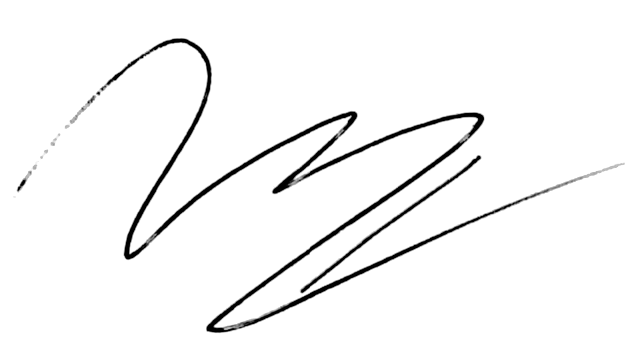
\includegraphics[height=2cm]{content/resources/signatures/nnknguyen.png} 
\vspace{2cm}
\\ Nguyễn Ngọc Khôi Nguyên \\
% 
\includegraphics[height=2cm]{content/resources/signatures/pnttung.png}
\vspace{2cm}
\\ Phan Nguyễn Thanh Tùng 
} \\
\hline
\end{longtable}

% 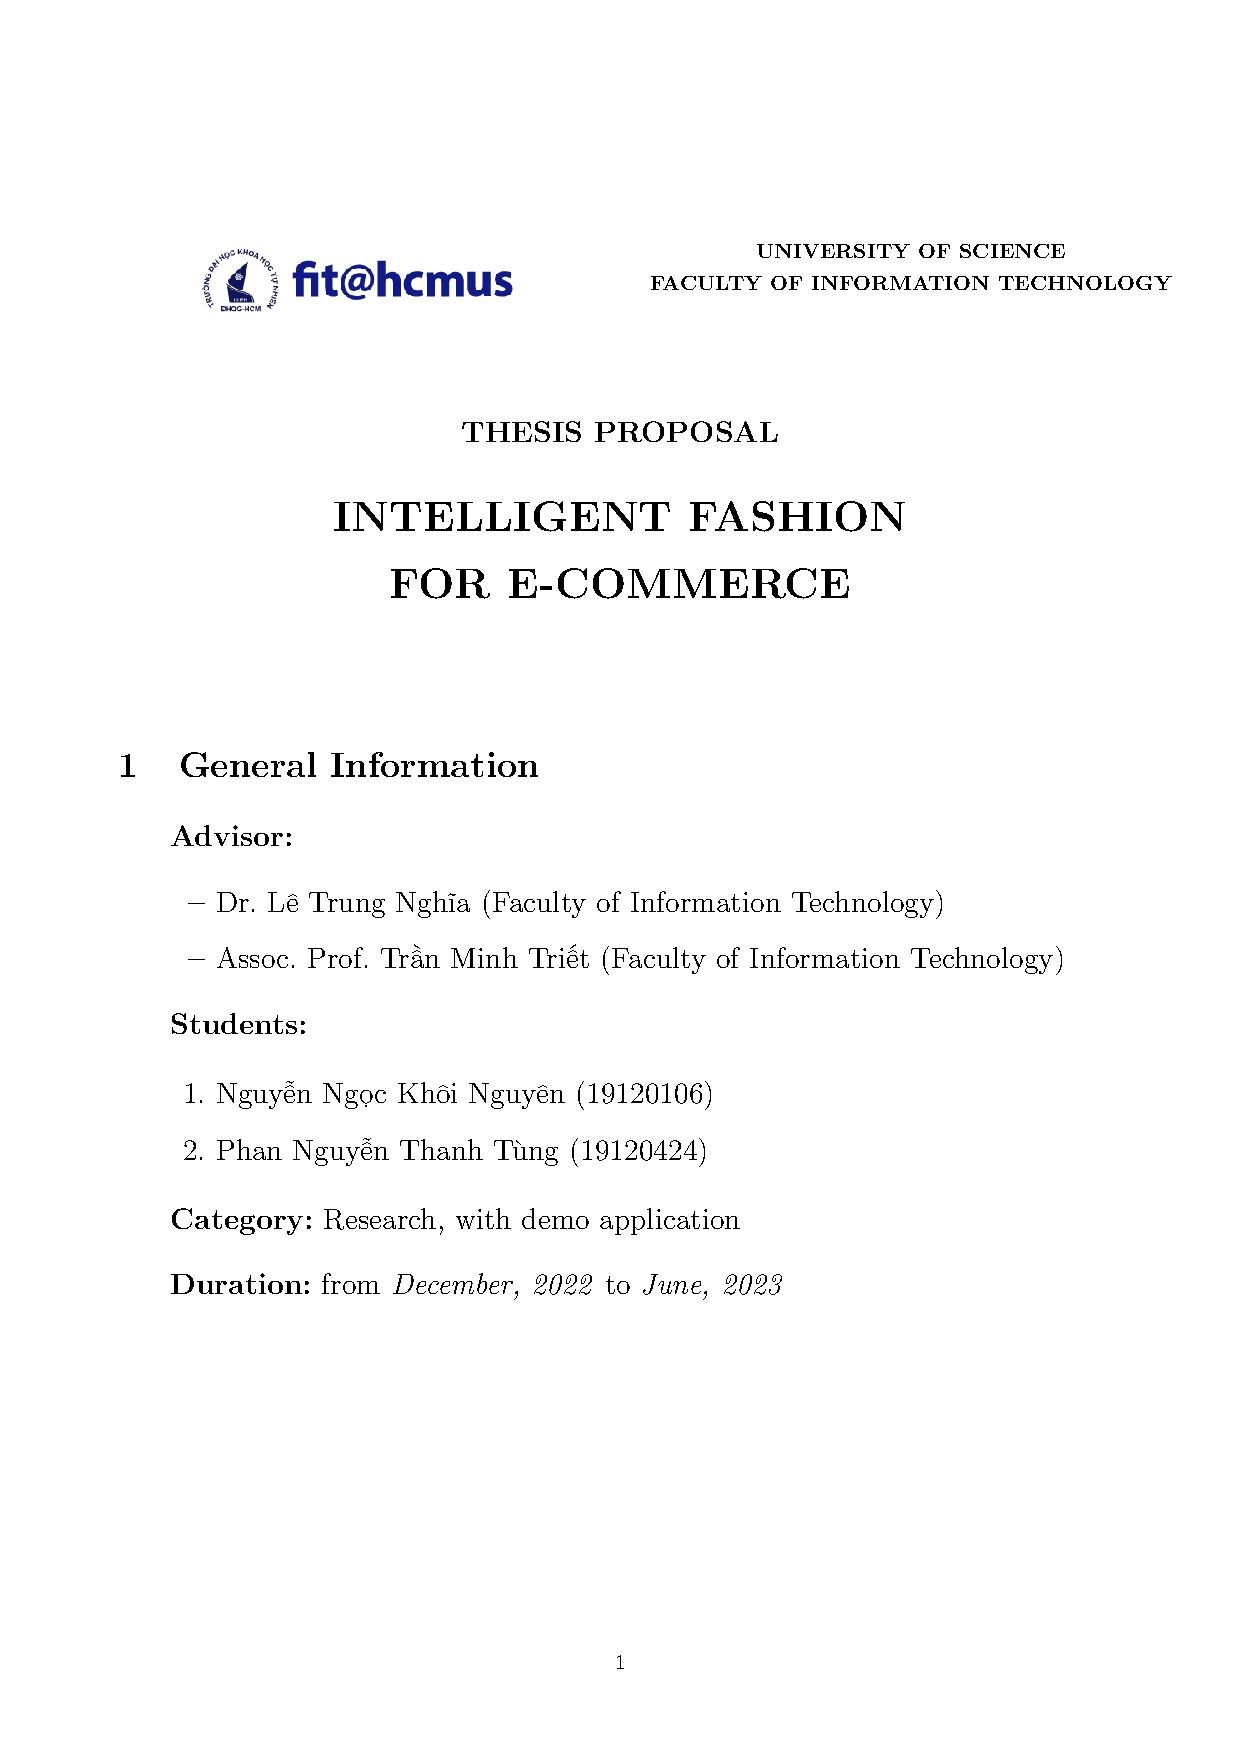
\includepdf[pages=-]{proposal.pdf}

\tableofcontents \clearpage
\listoftables \clearpage
\listoffigures \clearpage
% \listofalgorithms \clearpage
%%%%%%%%%%%%%%%%%%%%%%%%%%%%%%%%%%%%%%%%%%%%%%%%%%%%%%%
% You can comment out the following line if you don't
% have a "List of Plates"
%%%%%%%%%%%%%%%%%%%%%%%%%%%%%%%%%%%%%%%%%%%%%%%%%%%%%%%
% \listofplates \clearpage

%%%%%%%%%%%%%%%%%%%%%%%%%%%%%%%%%%%%%%%%%%%%%%%%%%%%%%%
% You can comment out the following line if you don't
% have a "List of Acronyms"
%%%%%%%%%%%%%%%%%%%%%%%%%%%%%%%%%%%%%%%%%%%%%%%%%%%%%%%
% \include{loa}

% Paragraph spacing
% \setlength\parskip{0.6em}
% Text-float spacing
\setlength\intextsep{24pt}
%%%%%%%%%%%%%%%%%%%%%%%%%%%%%%%%%%%%%%%%%%%%%%%%%%%%%%%
% Your Malay and English abstracts, each in one file.
%%%%%%%%%%%%%%%%%%%%%%%%%%%%%%%%%%%%%%%%%%%%%%%%%%%%%%%
% \input{abs-mal}
\begin{EnAbstract}
The fashion e-commerce industry has become an important part of people's lives worldwide. To achieve this, companies have continuously explored and employed technological advancements to provide their customers with positive and engaging shopping experiences. Within this context, the development of recommendation systems has emerged as a pivotal concern, aiming to enhance customer experiences by offering personalized suggestions aligned with individual preferences and styles. Furthermore, addressing the crucial need of online shoppers, virtual try-on technology enables users to visualise how specific garments would look when appearing on them, thereby elevating the customer experience and mitigating damaged item costs for retailers.

This thesis investigates two major challenges in fashion e-commerce: \textbf{fashion recommendation} and \textbf{virtual try-on}. Regarding recommendation problem, we explore various approaches for three types of retrieval: similar items retrieval within the same category, complementary items retrieval from different categories, and text feedback-guided item retrieval. Notably, our method for retrieving complementary items, based on the transformer architecture, has demonstrated its effectiveness through experimental evaluation. Furthermore, we enhance the overall performance of the search pipeline by integrating approximate algorithms, thereby optimizing the search process. As for the virtual try-on tasks, to address the speed limitations of previous methods, we propose a virtual try-on framework designed to be faster and more memory-efficient while still maintaining realistic output compared to predecessors. The main contribution is that we utilize the knowledge distillation technique, which uses a strong Teacher model to achieve a lightweight Student network.

To exemplify the potential of this thesis, we develop applications in two scenarios: a web-based Smart Fashion Assistant System for online shopping and an AR application for clothing try-on, namely Magic Mirror.


\end{EnAbstract}


\mainmatter

%%%%%%%%%%%%%%%%%%%%%%%%%%%%%%%%%%%%%%%%%%%%%%%%%%%%%%%
% The actual chapters of your thesis as listed in
% mainchaps.tex. Make sure you have the relevant
% chapter files.
% E.g. if you mainchaps.tex contains the lines
%
%  \include{hypothesis.tex}
%  \include{proof.tex}
%
% Then you MUST have the files hypothesis.tex, proof.tex
% (containing the relevant chapters) in the same directory
% as mainchaps.tex.
%%%%%%%%%%%%%%%%%%%%%%%%%%%%%%%%%%%%%%%%%%%%%%%%%%%%%%%
\chapter{Introduction}
\label{chapter-introduction}
\begin{ChapAbstract}
This chapter overviews e-commerce within fashion retail, focusing on the challenges associated with personalized and immersive experiences. We first discuss two significant online shopping problems, which involve virtual try-on technologies and fashion recommendation systems, and investigate various approaches to tackle those problems. Next, we describe the main contributions of this thesis to bridge the gap between physical and online fashion retail. Finally, the organizational structure of the thesis is presented, offering a concise overview of the subsequent chapters and their contents.
\end{ChapAbstract}

%%%%%%%%%%%%%%%%%%%%%%%%%%%%%%%%%%%%%%%%%%%%%%%%%%%%%%%%%%%%%%%%
\section{Overview}
Nowadays, the fashion industry has become an important part of people's lives. The development of digital globally and the recent pandemic has led to changes in consumer behaviour: e-commerce is increasingly popular and developed. Traditional retail shop owners also expand their stores on online platforms such as Amazon, Zalando, etc. Because of this, it is hardly surprising that the fashion e-commerce market will continue to flourish and diversify at an extraordinary pace. The global fashion e-commerce market is expected to reach a value of over 820 billion U.S. dollars in 2023 and could be 1.2 trillion U.S. dollars in 2027~\cite{Fashion2327-Statista2023} (details are shown in~\autoref{fig:market-forecast}). Nevertheless, the transition from traditional in-store shopping to online shopping presents distinctive challenges, such as the time-consuming process of item selection without some recommendations from the sales staff, limitations in trying on clothes before making a purchase, and risks and costs associated with product transportation.

\begin{figure}[h!]
    \centering
    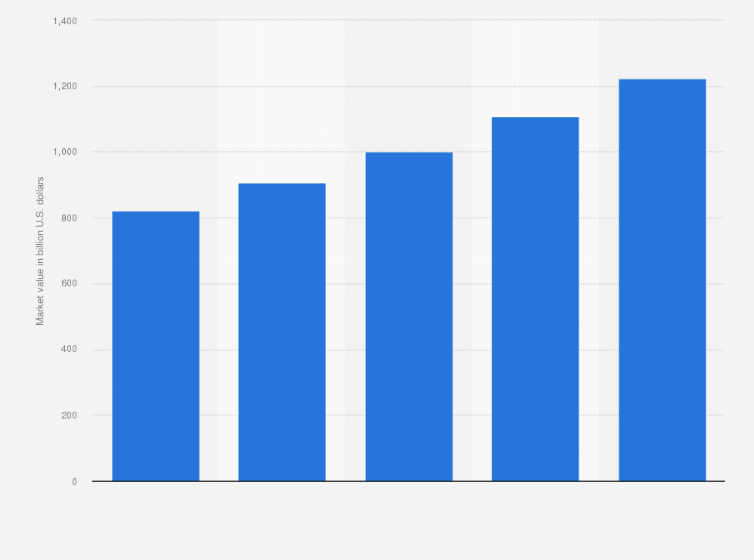
\includegraphics[width=0.7\linewidth]{content/resources/images/introduction/fashon-online-market.png}
    \caption{Fashion e-commerce market value worldwide forecast 2023-2027 (in billion U.S. dollars)~\cite{Fashion2327-Statista2023}.}
    \label{fig:market-forecast}
\end{figure}

In response to these challenges, intelligent fashion technologies have emerged as promising solutions to serve customers with the same support and comfort as in the in-person shopping experience. This thesis focuses on two significant areas of intelligent fashion: fashion recommendation systems and virtual try-on technologies. Both methodologies share a common objective of augmenting the customer experience on online platforms, thereby enabling retailers to bolster profitability. Fashion recommendation systems help users make easier and smarter shopping choices by recommending items that suit their preferences and style. Furthermore, virtual try-on technology has garnered significant attention in recent years by addressing a crucial concern of online shoppers: being concerned about how a particular in-shop garment will look when they wear it and whether it suits them. By allowing users to try on items virtually, this technology enhances the customer experience and saves the cost of damaged items for retailers. These solutions draw a new picture of online shopping and promise to take the customer experience to the next level.

%%%%%%%%%%%%%%%%%%%%%%%%%%%%%%%%%%%%%%%%%%%%%%%%%%%%%%%%%%%%%%%%
\section{Motivations}

Virtual try-on technology is a method to help customers visualize how a garment might look on their body based on an image of the person and an image of the desired item. This technology addresses a substantial challenge online shoppers encounter: having to visit a store to try on clothing items physically. According to a study of Coresight~\cite{web-try-on-motivation},  the period from March 2022 to March 2023 saw a notable 24.4\% average return rate for online clothing orders in the United States, which is equivalent to \$38 billion in returns. Moreover, 53\% of the respondents revealed that their primary reason for returns was the ill-fit of that garment during try-on (\cite{web-try-on-motivation}).

\begin{figure}[h!]
    \centering
    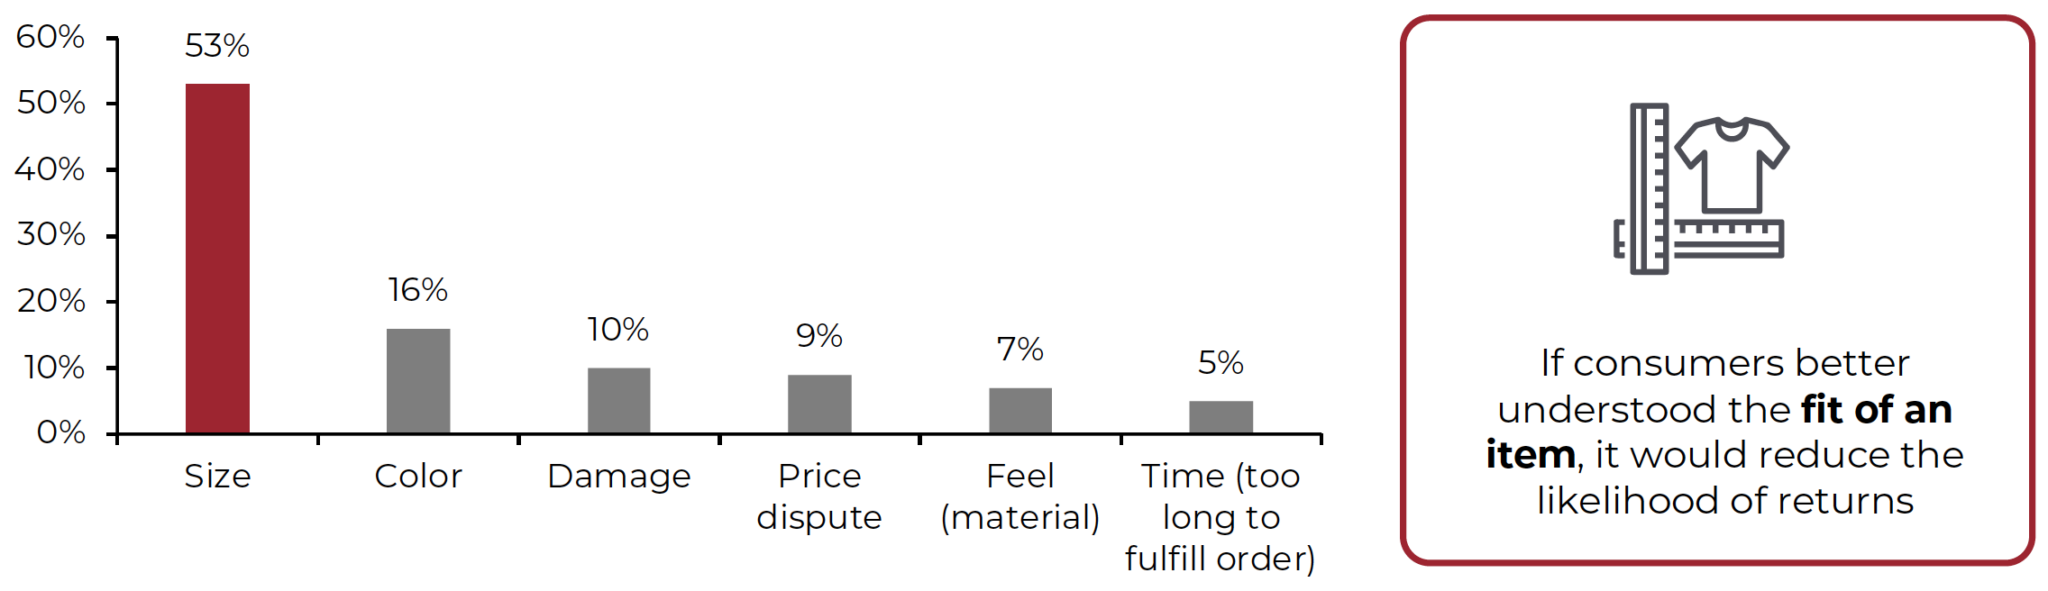
\includegraphics[width=0.7\linewidth]{content/resources/images/introduction/motivation-try-on.png}
    \caption{Reasons for garment returns from March 2022 to March 2023 (\% of Respondents)}
    \label{fig:try-on-motivation}
\end{figure}

As a result, there is a growing interest in virtual try-on, demonstrating the potential to enhance shopping experiences by integrating Augmented Reality (AR). However, existing works on image-based virtual try-on mostly do not put their concern about the complexity of their models, resulting in challenges when applying them in real-time scenarios. This motivates us to investigate the potential of a faster and more resource-efficient virtual try-on method while ensuring the fidelity of the outcomes. 

Fashion recommendation has always been crucial to modern fashion e-commerce systems due to its numerous benefits. According to a study of ViSenze~\cite{web-recommendation-motivation}, recommendations can increase conversion rates by up to 300\% and increase revenue by up to 31\%. It saves users valuable time and effort by curating multiple sets of items that align with their preferences and style. Instead of spending hours searching for fashion items online or in physical stores, users can rely on these recommendations to discover new and relevant clothes. Moreover, these recommendations help users explore a wider range of options, introducing them to different styles or brands. This encourages users to try out something they might not have considered before, thus improving the fashion industry's overall revenue. Additionally, as 71\% of consumers feel frustrated when their shopping experience is impersonal~\cite{web-recommendation-motivation}, fashion recommendation can simplify decision-making and increase user satisfaction by presenting curated options tailored to individual preferences. Ultimately, fashion recommendation has proven its usefulness by assisting users in discovering new styles, saving time, and making informed fashion choices.

%%%%%%%%%%%%%%%%%%%%%%%%%%%%%%%%%%%%%%%%%%%%%%%%%%%%%%%%%%%%%%%%
\section{Objectives and Main Contributions}
The primary objective of this thesis is to investigate and address two significant challenges in the field of fashion e-commerce: virtual try-on and fashion recommendation. By leveraging intelligent systems and cutting-edge method technologies, we aim to develop innovative solutions that enhance the online shopping experience and bridge the gap between the physical and digital realms of fashion retail.

To address the previous virtual try-on method issues, we aim to propose a framework that can achieve faster run time and less memory consumption while producing results of the same quality. Thus, it can pave the potential of integrating image-based virtual try-on into real-time AR scenarios.

Regarding the fashion recommendation problem, we focus on taking a fashion item as the reference item and recommending based on the visual features of that item. This research explores multiple approaches to produce meaningful results for such a problem. These approaches include intra-category similar item retrieval, inter-category complementary item retrieval, and text feedback-guided item retrieval. We also study incorporating approximate searching methods into these approaches to enhance the system's overall performance.

Another important objective of this thesis is to create an intelligent system for online shopping support, including web and AR applications. We aim to combine the power of fashion recommendation and virtual try-on in this system, offering new possibilities for personalized and immersive interactions between consumers and online fashion platforms.

The main contribution of this thesis can be summarized as follows:
\begin{itemize}
    \item Propose a virtual try-on framework based on knowledge distillation learning. We can achieve a lightweight network, reducing inference time and memory consumption, thus making it easier to deploy and operate on AR devices.
    \item Introduce an automatic fashion-pose data generation pipeline designed to enrich existing fashion datasets by synthesizing new person poses from a single image of that person.
    \item Investigate various ways to recommend fashion items from a reference image. These approaches include retrieving intra-category similar items, inter-category complementary items and text feedback-guided items. We also propose Outfit Retrieval Transformer to address the complementary item retrieval task.
    \item Incorporate approximate searching for retrieval, which runs significantly faster while producing nearly the same results as exhaustive methods.
    \item Build an AR application for virtual try-on, which can reduce the risk of damage to real clothes for shops.
    \item Develop a smart fashion assistant web application tailored for the fashion e-commerce industry, which integrates virtual try-on functionality and fashion recommendation capabilities, enhancing the overall user experience and increasing customer satisfaction in the fashion e-commerce sector. 
\end{itemize}


% The specific objectives of this research are as follows:


%%%%%%%%%%%%%%%%%%%%%%%%%%%%%%%%%%%%%%%%%%%%%%%%%%%%%%%%%%%%%%%%
\section{Thesis Organization}

This thesis is organized into 7 chapters: 

\textbf{Chapter 1}: This chapter overviews e-commerce within fashion retail, focusing on the challenges associated with personalized and immersive experiences. We first discuss two significant online shopping problems, which involve virtual try-on technologies and fashion recommendation systems, and investigate various approaches to tackle those problems. Next, we describe the main contributions of this thesis to bridge the gap between physical and online fashion retail. Finally, the organizational structure of the thesis is presented, offering a concise overview of the subsequent chapters and their contents.

\textbf{Chapter 2}: This chapter provides an overview of the fundamental knowledge relevant to our thesis. We present a list of Computer Vision problems that play important roles in our proposed approach.

\textbf{Chapter 3}: This chapter presents an overview of the literature in the virtual try-on and fashion recommendation fields. In the domain of virtual try-on, we introduce recent image virtual try-on approaches. Besides, some commercial products and their technology are discussed to provide a comprehensive view of this field. Moving on to fashion recommendation, we introduce related works centering on visual-based fashion recommendations. Finally, we discuss techniques for similarity search, including exhaustive and approximate methods applied to our recommendation approaches.

\textbf{Chapter 4}: In this chapter, we propose Distilled Mobile Real-time Virtual Try-On (DM-VTON), which focuses on synthesizing try-on images with increased speed compared to previous methods while ensuring accuracy. Our approach is based on a knowledge distillation scheme that leverages a strong Teacher network as supervision to guide a Student network without relying on human parsing. Notably, we introduce an efficient Mobile Generative Module within the Student network, significantly reducing the runtime while ensuring high-quality output. Additionally, we propose Virtual Try-on-guided Pose for Data Synthesis to address the limited pose variation observed in training images. Finally, we provide the experimental details of our proposed method, and then we present a comparative study of DM-VTON with state-of-the-art methods.

\textbf{Chapter 5}: In this chapter, we address the problem of recommending items given a reference fashion item. We carefully investigate three approaches to retrieving items: similar items within the same category, complementary items from other categories, and items guided by text feedback. 
In terms of retrieving intra-category similar items and text feedback-guided items, we employ a pretrained CLIP-based model and receive remarkable results. As for the inter-category complementary item retrieval, we consider it a Natural Language Process problem and propose Outfit Retrieval Transformers (ORT), which utilizes the Transformers architecture. Through experiments, ORT proves its effectiveness and can produce reasonable recommendations. Because using an embedding to query items from a dataset plays an important role in recommendation, we analyze various approximate searching methods and compare them with the exhaustive K-Nearest Neighbor algorithm regarding query time and accuracy.

\textbf{Chapter 6}: This chapter presents our applications that assist customers in e-commerce based on the methods presented, including Smart Fashion Assistant, a system for online shopping support, and Magic Mirror, an application that allows users to try on clothing items virtually in an augmented reality scenario. We present an overview of each application, followed by the details of the conducted experiments, including a pilot study to evaluate their effectiveness and user satisfaction.

\textbf{Chapter 7}: We conclude our work by summarizing the results obtained and discussing the potential for future research directions. In this thesis, we solve two major problems in online fashion shopping: virtual try-on and fashion recommendation. Through intensive experiments, we prove the applicability and efficiency of our solutions and further demonstrate them in demo applications. The feedback we gained from the pilot study shows that our work still has some limitations, which we plan to improve in future works.
\chapter{Background}
\label{chapter-background}
\begin{ChapAbstract}
This chapter provides an overview of the fundamental knowledge relevant to our thesis. We present a list of Computer Vision problems that play important roles in our proposed approach.
\end{ChapAbstract}

\section{Convolution Neural Network}
Convolutional neural network, also known as CNN or ConvNet, was introduced by Yann LeCun et al.~\cite{LeCun-NC1989-Backpropagation} to understand and explain visual data such as images. A digital image contains pixels arranged in a grid to represent information about colour, brightness, texture, etc. The CNN network is inspired by how the human visual system processes data on each receptive field. CNN is commonly used for extracting feature maps from images containing information about the relationship between pixels. This information can be used as the input for the downstream tasks: image classification, object detection, etc.

\subsection{Convolution Layer}
The convolution Layer is the core block of a CNN. It extracts information from the input through matrix multiplications. Specifically, it performs multiplications between a set of learnable parameters, known as a kernel, and the corresponding matrix bounded by the receptive fields. In mathematics, the convolution between two functions~\cite{Rudin-McGrawHill1991-Functional}, $f, g: \mathbb{R}^d \rightarrow \mathbb{R}$ is defined as:

\begin{equation}
    (f \ast g)(x) = \int f(z)g(x - z)dz,
\end{equation}

For two-dimensional matrices, we have the formula:
\begin{equation}
    (f \ast g)(i, j) = \sum_{a}^{A-1}\sum_{b}^{B-1}f(a, b)g(i - a, j - b),
\end{equation}
Where f is the kernel and g is the input image with size $A \times B$. An illustration of the formula is shown in~\autoref{fig:chapter2-convolution-compute}.

\begin{figure}[h!]
    \centering
    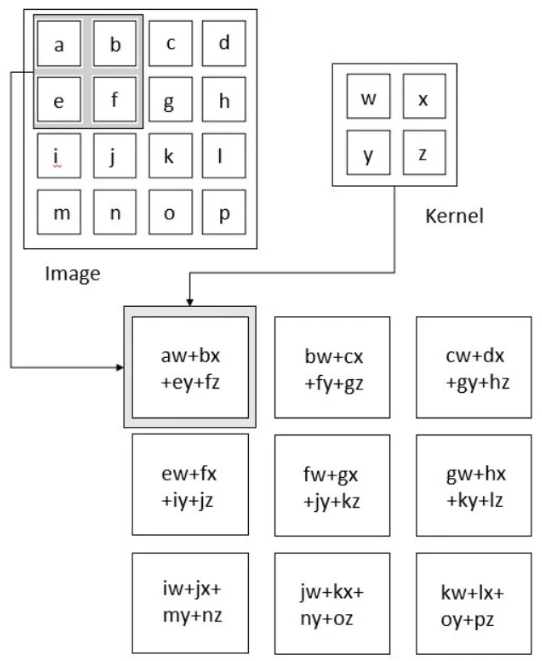
\includegraphics[width=0.5\linewidth]{content/resources/images/background/convolution-compute.png}
    \caption{Convolution operation (Source: Deep Learning~\cite{Goodfellow-MIT2016-DL}).}
    \label{fig:chapter2-convolution-compute}
\end{figure}

Visually, the convolution window (kernel) is slid over all the height and width of images to compute the result at each spatial position. However, with this method, we can only shift the kernel pixel by pixel, leading to high computational costs when the input size is large. Stride and padding are techniques applied in convolution for computational efficiency and to control the downsampling rate. Stride is the number of elements that the window moves at a time. It enables to capture a larger receptive field. Padding is the extra pixels added around the border of the input before performing the convolution operation to keep the input dimensions after convolution. If we have an input of size $W_{in} \times H_{in}$ and kernel of size $F$ with stride $S$ and padding $P$, then the size of output is $W_{out} \times H_{out}$ (as illustrated in~\autoref{fig:chapter2-convolution}):
\begin{equation}
    \begin{cases} 
        W_{out} = \dfrac{W_{in} - F + 2P}{S} + 1 \\ 
        H_{out} = \dfrac{H_{in} - F + 2P}{S} + 1 
    \end{cases}.
\end{equation}

\begin{figure}[h!]
    \centering
    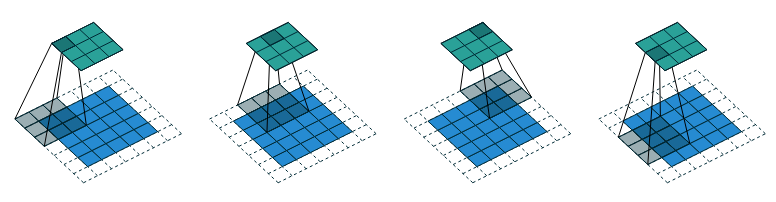
\includegraphics[width=\linewidth]{content/resources/images/background/convolution.png}
    \caption{Two-dimensional convolution ($F=3, S = 2, P = 1$) with input of size $W_{in} = H_{in} = 5$. After sliding the kernel over all the input, we get the output with size  $W_{out} = H_{out} = 3$ (Source: A guide to convolution arithmetic for deep learning~\cite{Dumoulin-ArXiv2016-Guide}).}
    \label{fig:chapter2-convolution}
\end{figure}

\subsection{Pooling Layer}
The pooling layer is commonly inserted between successive convolution layers to reduce the spatial size of the feature maps by aggregating information from local regions. This help decreases the number of parameters and computation and prevents overfitting. The pooling operation uses a window slid over all the input to compute an output for each region. Unlike the convolution layer, the window of the pooling layer contains no parameters. Instead, the output of the regions in the window is determined by a unified function, such as the maximum or the average of the neighbours in the pooling window area. 

The pooling operation is processed independently on every depth slice of the input. If we have an input of size $W_{in} \times H_{in} \times D_{in}$ and a pooling window with size $F$ and stride $S$, the pooling layer produces an output of size $W_{out} \times H_{out} \times D_{out}$ ($D_{in}, D_{out}$ are the depth size) where:
\begin{equation}
    \begin{cases} 
        W_{out} = \dfrac{W_{in} - F}{S} + 1 \\ 
        H_{out} = \dfrac{H_{in} - F}{S} + 1 \\
        D_{out} = D_{in}
    \end{cases}.
\end{equation}

\begin{figure}[h!]
    \centering
    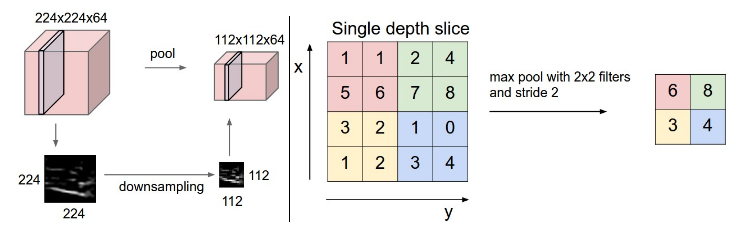
\includegraphics[width=\linewidth]{content/resources/images/background/maxpool.png}
    \caption{Pooling operation downsample by applying the kernel to each slice. \textbf{Left}: Appling pooling operation with $F = 2, S = 2$ reduces the input size from $224x \times 224 \times 64$ to  $112x \times 112 \times 64$. \textbf{Right}: Illustration of the max pooling with $F = 2, S = 2$, which preserves the maximum value in adjacent pixels (Source: CS231n: Deep Learning for Computer Vision~\cite{Stanford-CS231n}).}
    \label{fig:chapter2-maxpool}
\end{figure}


\section{Attention and Transformer}
\subsection{Self-attention}
Self-attention is a sequence-to-sequence operation: the input is a sequence of vectors that goes in, and the output is also a sequence of vectors. This operation is proposed in the paper "Attention is all you need" \cite{Vaswani-NeurIPS2017-Attention}. We denote the input vectors as $x_1, x_2, ..., x_t$ and the corresponding output vectors $y_1, y_2, ..., y_t$. All vectors have dimension k.

The self-attention operation takes a weighted average over all the input vectors, as in \autoref{eq:self-attention}. The weight values can be derived from the input vectors themselves, which is why this operation is called self-attention. \autoref{eq:self-attention-weight} shows the simplest option, the dot product.

\begin{equation}
y_i = \sum_{j} w_{ij} x_j,
\label{eq:self-attention}
\end{equation}

\begin{equation}
w_{ij} = \dfrac{exp(w'_{ij})}{\sum_{j} exp(w'_{ij})},
\end{equation}

\begin{equation}
w'_{ij} = x^T_ix_j.
\label{eq:self-attention-weight}
\end{equation}

Modern deep-learning architectures further improve this operation by adding three $k x k$ learnable matrices, denoted as $W_q$, $W_k$, and $W_v$. We apply these matrices as the linear transformations of the input vectors $x_i$. \autoref{eq:self-attention-modern} shows the specific formula.

\begin{equation}
y_i = \sum_{j} w_{ij} (W_v x_j),
\label{eq:self-attention-modern}
\end{equation}

\begin{equation}
w_{ij} = \dfrac{exp(w'_{ij})}{\sum_{j} exp(w'_{ij})},
\end{equation}

\begin{equation}
w'_{ij} = (W_qx_i)^T(W_kx_j).
\end{equation}


\subsection{Multi-head Self-attention}
Using a single self-attention operation, each input vector $x_j$ can only influence every output vector $y_i$ in a fixed way, depending on the transformation matrices $W$. To tackle this problem, Vaswani et al.\cite{Vaswani-NeurIPS2017-Attention} combine multiple self-attention mechanisms (indexed with $r$), which involve learning different matrices $W^r_k, W^r_q,$ and $W^r_v$. These are called attention heads $h$. Each attention head gives different output vectors $y^r_i$. These vectors are concatenated along all attention heads and passed through a linear transformation to reduce the dimension to $k$. \autoref{fig:chapter2-multihead} illustrates how multi-head self-attention works.

\begin{figure}[h!]
    \centering
    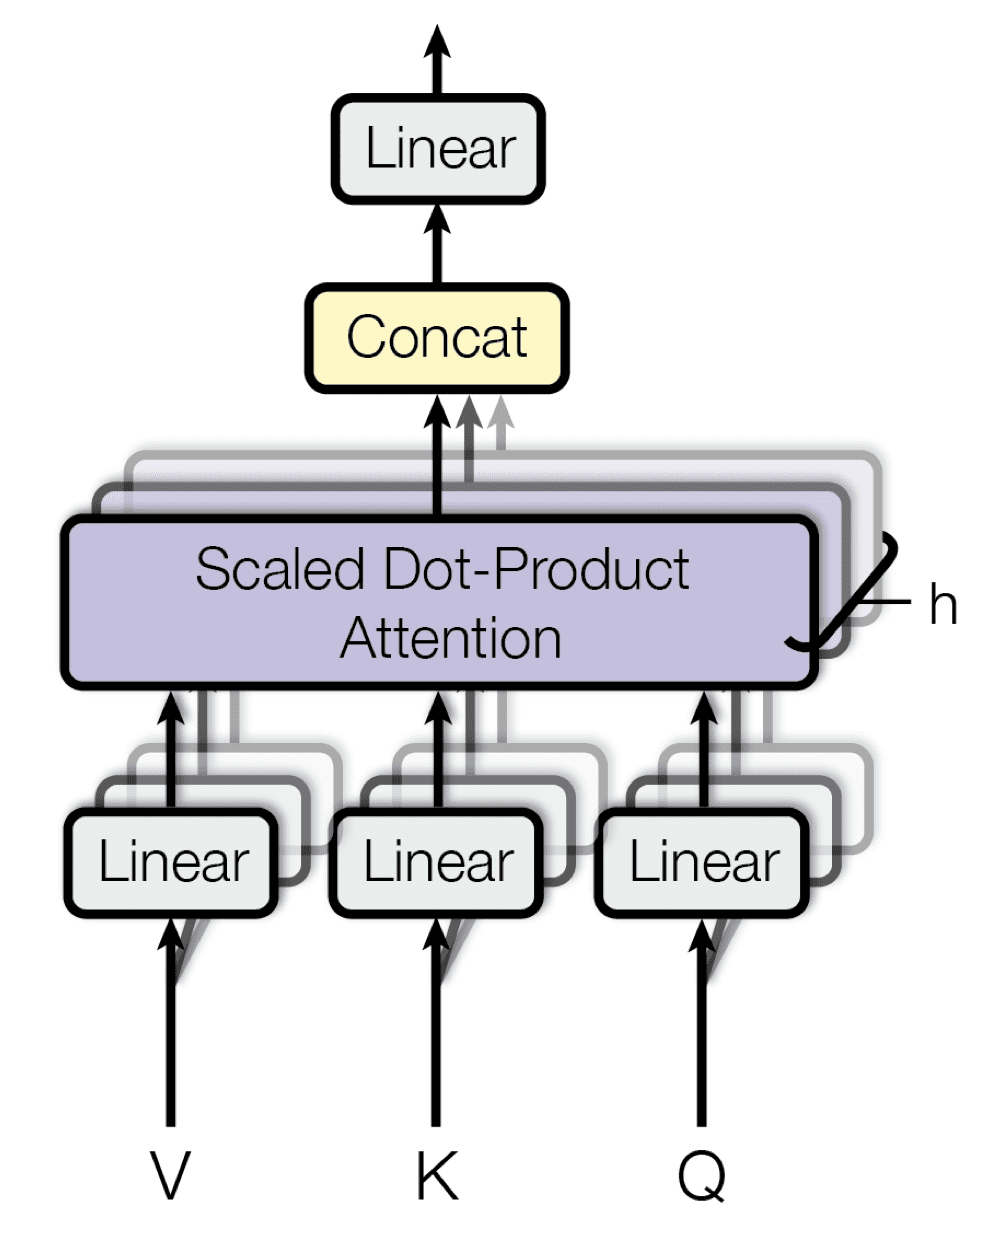
\includegraphics[width=0.3\linewidth]{content/resources/images/background/multihead.png}
    \caption{Multi-head self-attention mechanism (Source: Attention is all you need~\cite{Vaswani-NeurIPS2017-Attention}).}
    \label{fig:chapter2-multihead}
\end{figure}

However, this approach has one drawback, which takes $h$ times slower as the number of heads increases. Multi-head self-attention solves this problem by slicing the input vectors into $h$ chunks and performing the multi-head self-attention on each chunk. For example, if we have 640-dimension input vectors and 16 attention heads, we need to slice each input vector into 16 chunks of 40 dimensions. 

\subsection{Transformers}

Each transformer's block is built upon a multi-head self-attention block, followed by a normalization layer, a single multi-layer perception applied independently to each input vector, and another normalisation layer. Residual connections are added before both normalizations. \autoref{fig:chapter2-transformer} shows the architecture of a Transformers block.

\begin{figure}[h!]
    \centering
    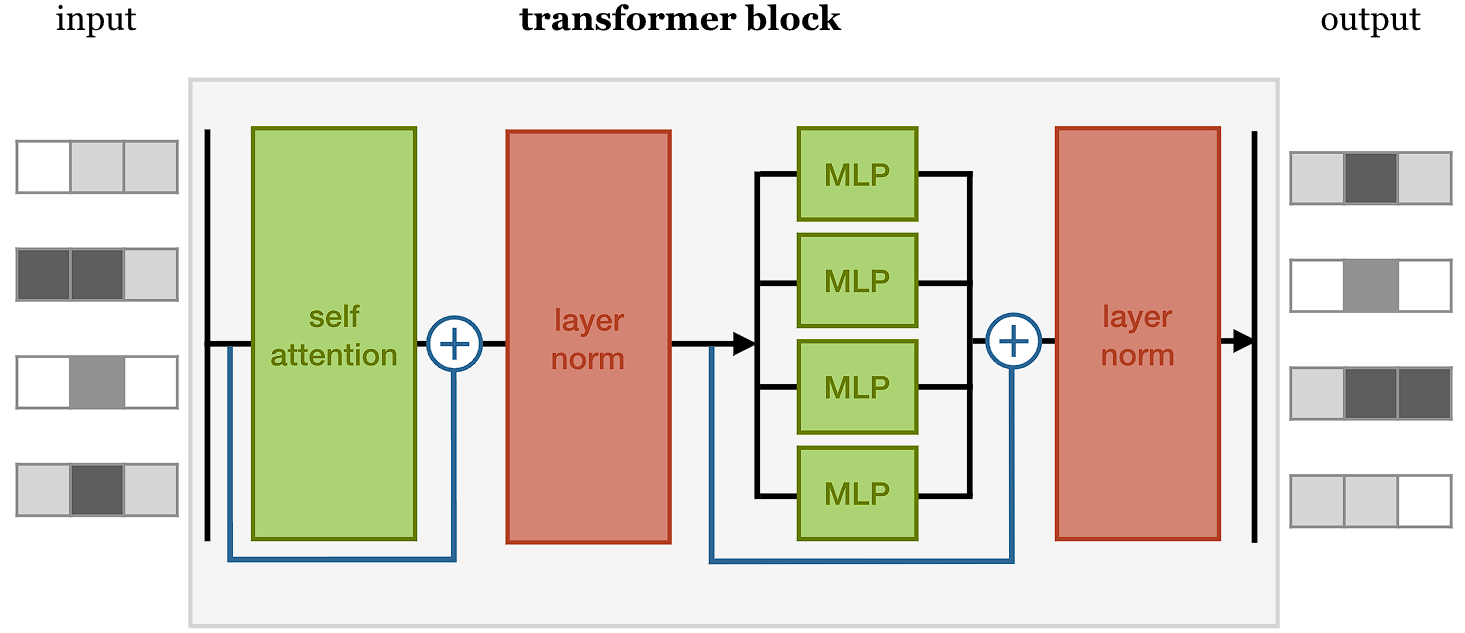
\includegraphics[width=\linewidth]{content/resources/images/background/transformers.PNG}
    \caption{Transformers block architecture (Source: Transformers from scratch~\cite{web-transform-from-scratch}).}
    \label{fig:chapter2-transformer}
\end{figure}

A \textbf{Transformers block} can produce a sequence of vectors given a sequence of vectors, so it is also a sequence-to-sequence model. Modern deep-learning architectures~\cite{Vaswani-NeurIPS2017-Attention, Devlin-ArXiv2018-BERT} utilize this characteristic and apply multiple Transformers blocks sequentially, called \textbf{Transformers Encoder}, to improve the overall performance.

Especially, in BERT~\cite{Devlin-ArXiv2018-BERT}, the author uses a special vector \textit{<CLS>} as the first input vector. The Transformers Encoder is trained so that the first output vector captures the semantics of the whole sequence of input vectors (\autoref{fig:chapter2-bert}). After being proposed, this approach is widely adopted for downstream tasks, such as classification, which require one embedding representing the whole input.

\begin{figure}[h!]
    \centering
    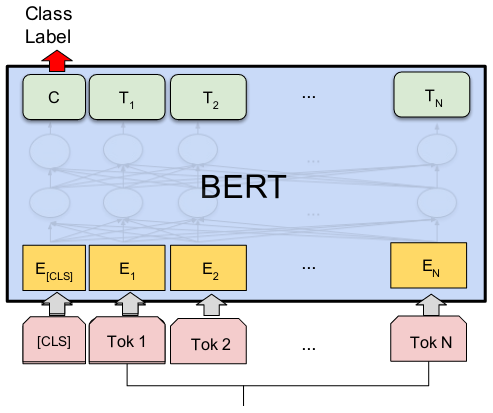
\includegraphics[width=0.7\linewidth]{content/resources/images/background/bert_class.png}
    \caption{BERT \textit{<CLS>} vector (Source: Text classification using BERT~\cite{web-bert}).}
    \label{fig:chapter2-bert}
\end{figure}

\chapter{Literature Review}
\label{chapter-literature-review}
\begin{ChapAbstract}
This chapter presents an overview of the literature in the virtual try-on and fashion recommendation fields. In the domain of virtual try-on, we introduce recent image virtual try-on approaches. Besides, some commercial products and their technology are discussed to provide a comprehensive view of this field. Moving on to fashion recommendation, we introduce related works centering on visual-based fashion recommendations. Finally, we discuss techniques for similarity search, including exhaustive and approximate methods applied to our recommendation approaches.
\end{ChapAbstract}
 %%%%%%%%%%%%%%%%%%%%%%%%%%%%%%%%%%%%%%%%%%%%%%%%%%%%%%%%%%%%%%%%
\section{Virtual Try-on}
This section presents the virtual try-on approaches, divided into two main parts. In the first one, we discuss the research on image-based virtual try-on, which aim to warp the garment to fit the target person's pose. After that, we introduce some commercial products that are being applied in practice and their limitations.

\subsection{Image-based Virtual Try-on}
Image-based virtual try-on techniques can be classified into two categories: parser-based and parser-free approaches, in the sense that they use a body-parser map in the inference process or not. Both of them typically involves three steps: extracting the intrinsic input features, warping the input garment to fit the clothing area of the person image, and performing the replacement using a generative model.

% \subsection{Parser-based Approach}
\paragraph{Parser-based Methods.} As for parser-based virtual try-on methods, they require human representation, including the human segmentation map, human pose, etc., to deform and fit the garment to the corresponding region on the input image. Previous methods~\cite{Han-CVPR2018-Viton, Wang-ECCV2018-Toward, Han-ICCV2019-Clothflow, Yang-CVPR2020-Towards, Fele-WACV2022-CVTON, Bai-ECCV2022-Single} utilized pretrained models such as human parsing~\cite{Gong-CVPR2017-Look, Li-TPAMI2020-Self}, pose estimation~\cite{Cao-CVPR2017-Realtime}, densepose~\cite{Guler-CVPR2018-DensePose} to extract information (i.e. human segmentation map) from the person input used for both training and inference.

The initial approach that laid the foundation for this method was VITON~\cite{Han-CVPR2018-Viton}, which proposed a coarse-to-fine framework. Firstly, a multi-task encoder-decoder generator is employed to generate a coarse sample and a clothing mask. Subsequently, the garment is warped using a thin plate spline (TPS) transformation with shape context matching. Finally, the coarse results are refined using a refinement network that leverages realistic details from a deformed item. Then it was realized that using image descriptors for warping had shown lower accuracy than deep learning networks. CP-VTON~\cite{Wang-ECCV2018-Toward}, building upon VITON~\cite{Han-CVPR2018-Viton}, adopted a similar architecture but utilized an end-to-end neural network to learn the transformation parameters of the TPS transformation. This improvement significantly enhanced the accuracy of the virtual try-on outcomes. 

\begin{figure}[h!]
    \centering
    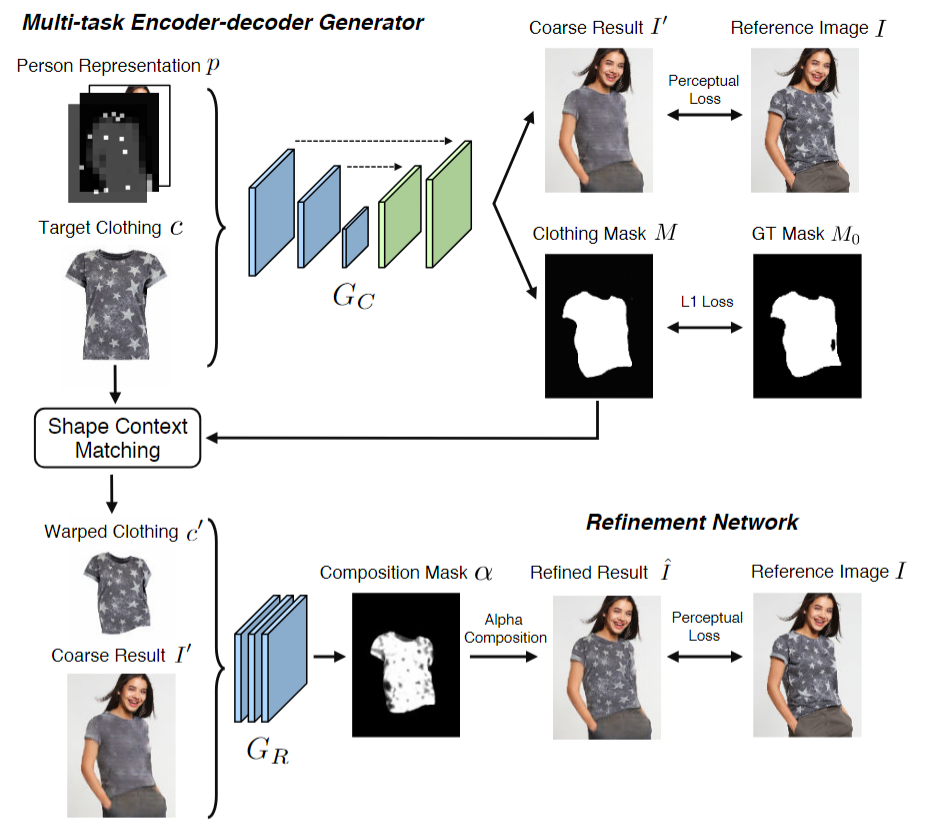
\includegraphics[width=0.7\linewidth]{content/resources/images/literature-review/viton.png}
    \caption{Overview architecture of VITON~\cite{Han-CVPR2018-Viton}.}
    \label{vton-viton}
\end{figure}

\begin{figure}[h!]
    \centering
    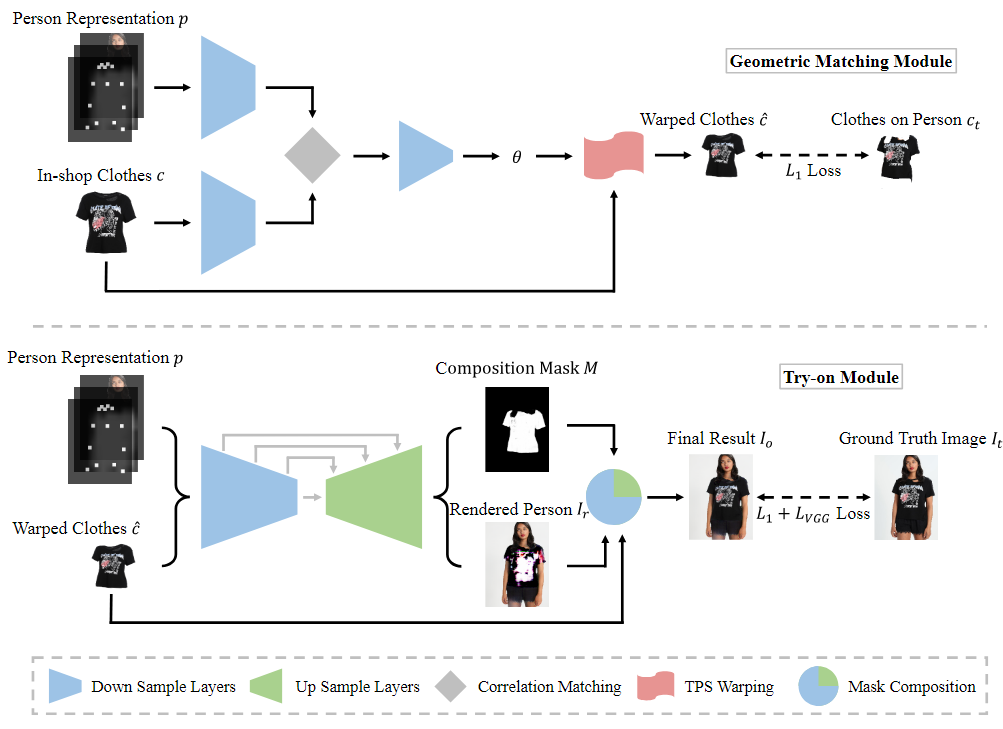
\includegraphics[width=0.85\linewidth]{content/resources/images/literature-review/cp-vton.png}
    \caption{Overview architecture of CP-VTON~\cite{Wang-ECCV2018-Toward}.}
    \label{vton-cpvton}
\end{figure}

Nonetheless, VITON~\cite{Han-CVPR2018-Viton} and CP-VTON~\cite{Wang-ECCV2018-Toward} only focus on deforming the target garment during the virtual try-on process. Consequently, these approaches lead to losing important details related to the human body when try-on. To mitigate this issue, Yang et al.~\cite{Yang-CVPR2020-Towards} proposed ACGPN, a framework that involves transforming the body-parser map to align with the target garment. Subsequently, the transformed parser map, input person image, and the deformed garment are utilized in the try-on generation. This integrated strategy ensures that the resulting try-on outcome effectively preserves the characteristics of both the human body and the in-shop clothes, enhancing the realism and fidelity of the try-on result.

\begin{figure}[h!]
    \centering
    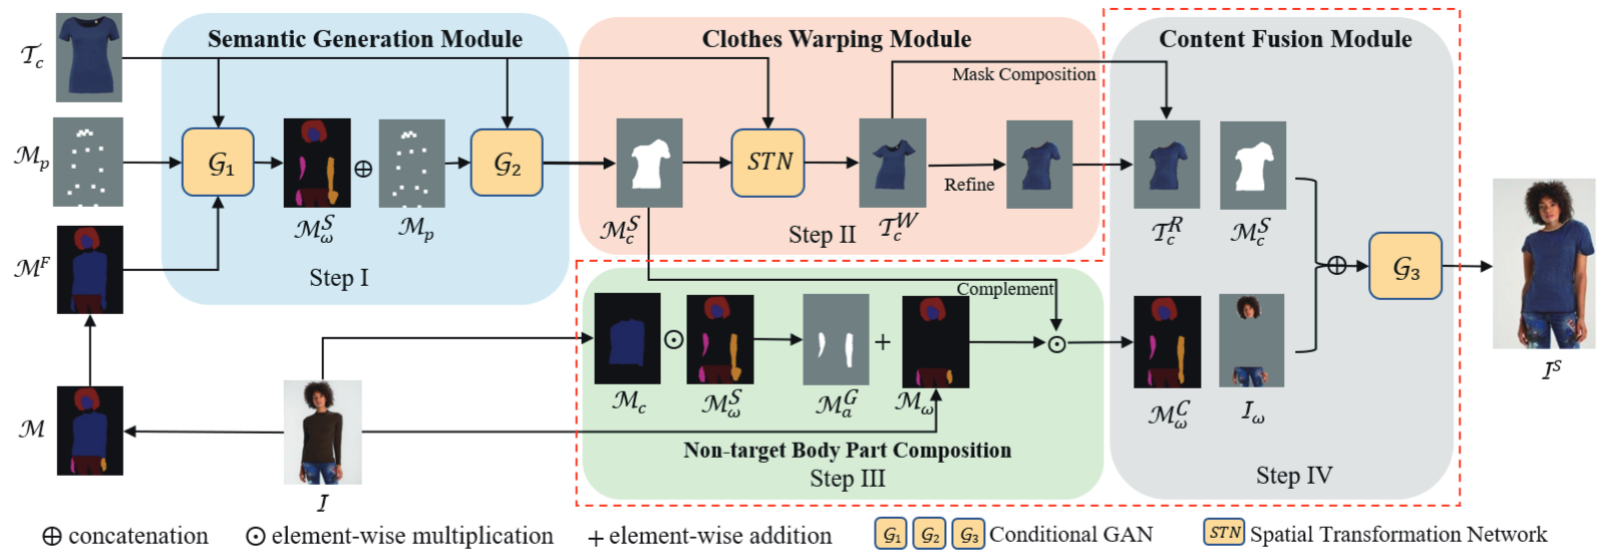
\includegraphics[width=\linewidth]{content/resources/images/literature-review/acgpn.png}
    \caption{Overview architecture of ACGPN~\cite{Yang-CVPR2020-Towards}.}
    \label{fig:vton-acgpn}
\end{figure}

Han et al.~\cite{Han-ICCV2019-Clothflow} introduced ClothFlow, a framework designed for synthesizing clothed person images, serving both posed-guided person image generation and virtual try-on tasks. First, similar to ACGPN~\cite{Yang-CVPR2020-Towards}, ClothFlow generates a segmentation map of the target person. Subsequently, a flow estimation network predicts the appearance flow~\cite{Zhou-ECCV2016-AppearanceFlow} that facilitates the warping of the source image to the desired target view. This approach yields more natural results compared to traditional TPS transformation. Finally, the final synthesized output is obtained by combining the source image, warped image, target segmentation map, and target pose. The ClothFlow framework for pose-guided person image generation is illustrated in~\autoref{fig:vton-clothflow}. For the virtual try-on tasks, the authors treated the garment image as the source image, and the input person pose as the target pose. The garment is then deformed by leveraging the predicted flow between the garment and the corresponding region of the person. The idea of using appearance flow instead of TPS transformation for deformation has been further developed and adopted by recent state-of-the-art methods~\cite{Ge-CVPR2021-Parser, He-CVPR2022-Style}.

\begin{figure}[h!]
    \centering
    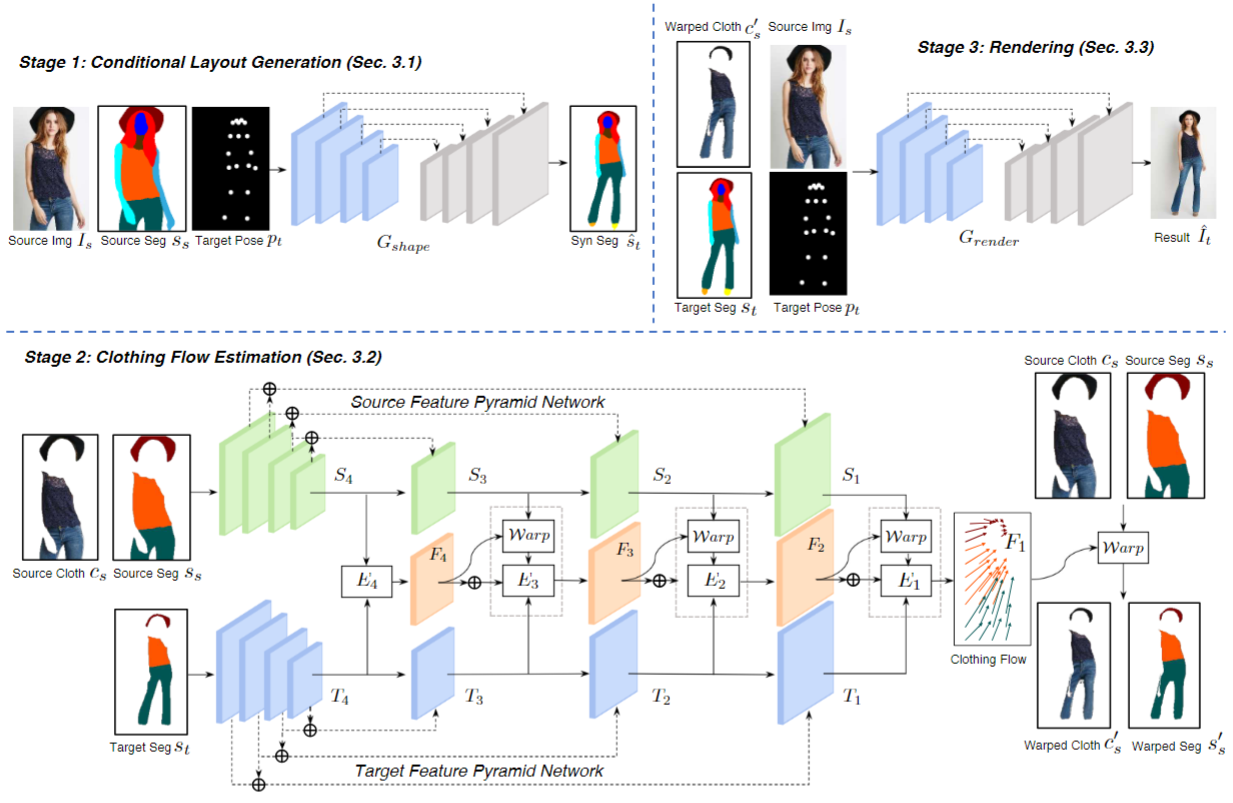
\includegraphics[width=\linewidth]{content/resources/images/literature-review/clothflow.png}
    \caption{Overview architecture of CLothFlow for pose-guided person image generation~\cite{Han-ICCV2019-Clothflow}.}
    \label{fig:vton-clothflow}
\end{figure}

Following the direction of multi-stage approaches, Fele et al.~\cite{Fele-WACV2022-CVTON} introduced a Context-driven Virtual Try-on Network (C-VTON). This framework comprises two fundamental components: a Body-Part Geometric Matcher, designed to deform the garment, and a Context-Aware Generator, aiming at generating the try-on image with contextual information.

\begin{figure}[h!]
    \centering
    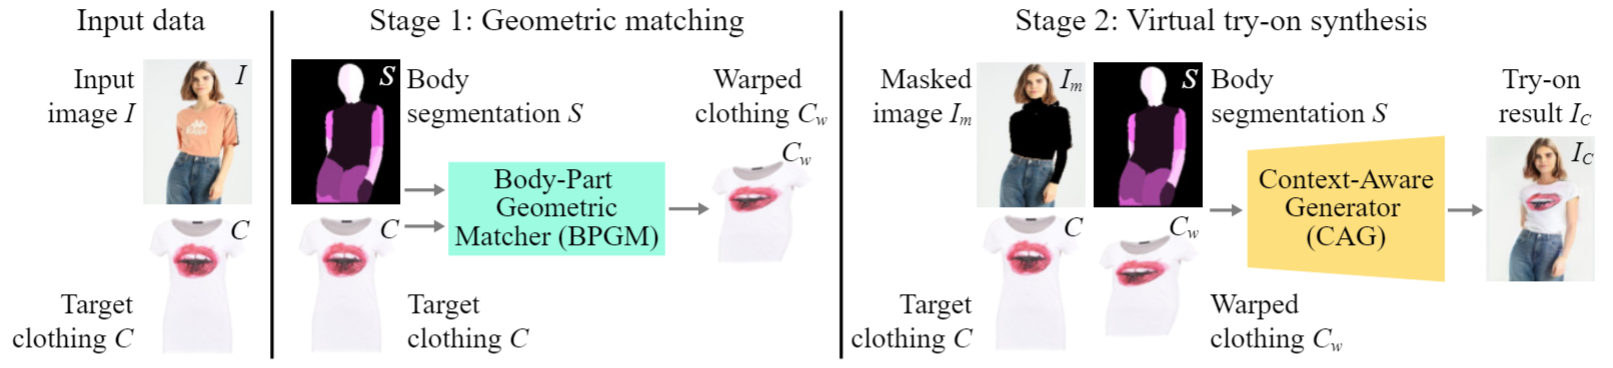
\includegraphics[width=\linewidth]{content/resources/images/literature-review/cvton.png}
    \caption{Overview architecture of C-VTON~\cite{Fele-WACV2022-CVTON}.}
    \label{fig:vton-cvton}
\end{figure}

However, the multi-stage approaches generate a try-on image relying on intermediate prediction results, which may be inaccurate, ultimately giving rise to noticeable artifacts in the final output. To address this issue, Bai et al.~\cite{Bai-ECCV2022-Single} introduced a novel Single Stage Virtual Try-on framework (SDAFN), which only uses a target pose map as guidance. By developing the deformable attention flow network and the shallow encoder and decoder, SDAFN allows the generation of try-on images end-to-end. The overall framework is shown in~\autoref{fig:vton-sdafn}.

\begin{figure}[h!]
    \centering
    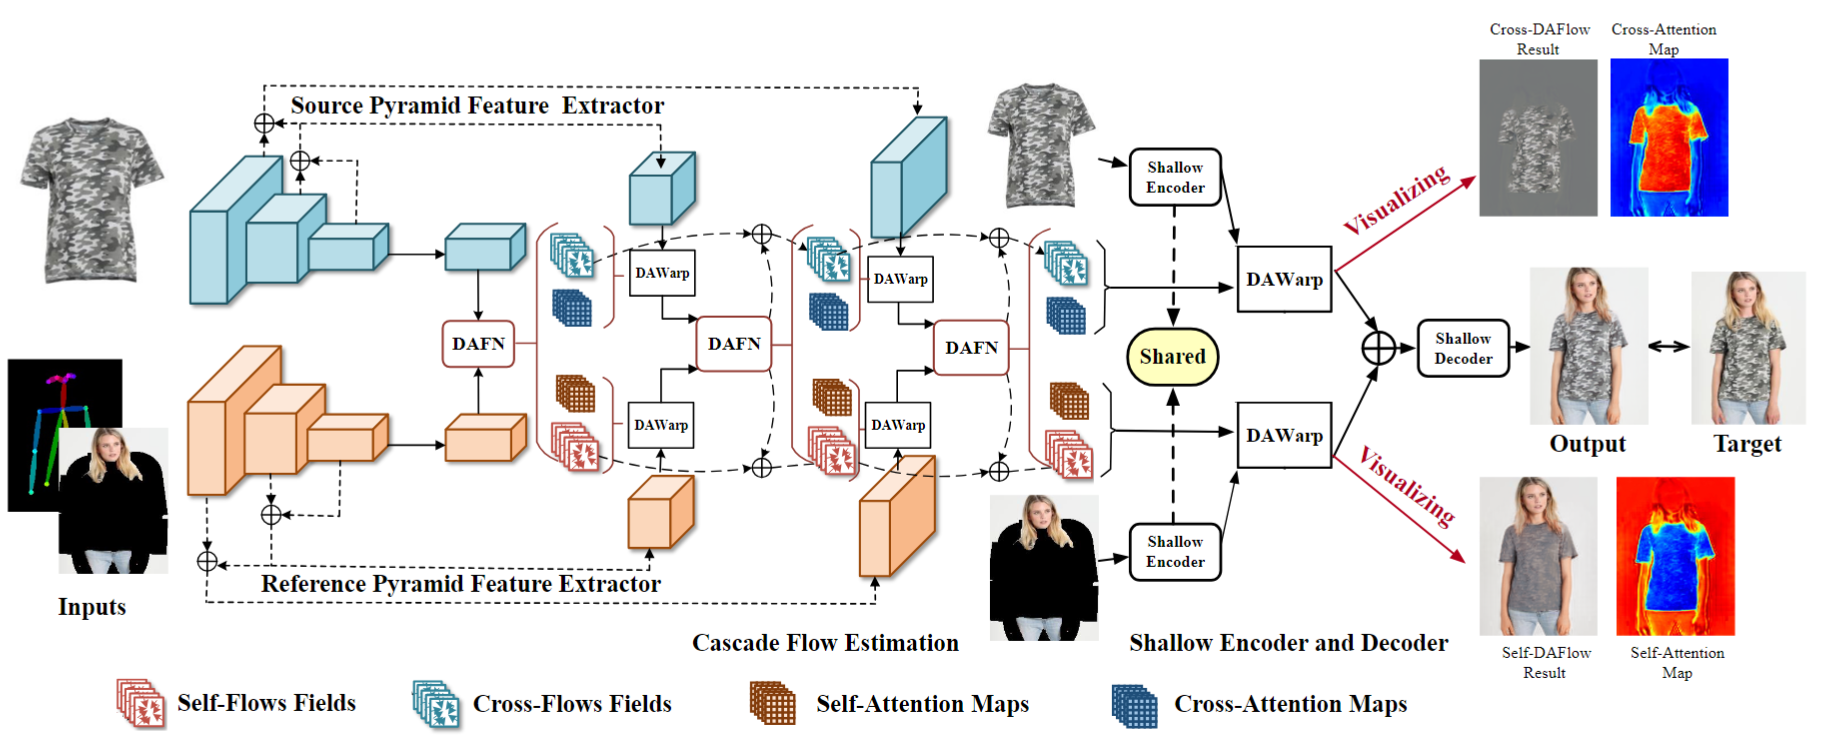
\includegraphics[width=\linewidth]{content/resources/images/literature-review/sdafn.png}
    \caption{Overview architecture of SDAFN~\cite{Bai-ECCV2022-Single}.}
    \label{fig:vton-sdafn}
\end{figure}

% \subsection{Parser-Free Approach}
\paragraph{Parser-free Methods.} In contrast, the parser-free approach only requires a person image and an input garment for inference. Consequently, this speeds up the process and eliminates reliance on human representation estimation models during inference. WUTON~\cite{Issenhuth-ECCV2020-Do}, as the pioneering parser-free method, introduced a Teacher-Student framework. It leverages a pretrained parser-based Teacher network to synthesize fake images acting as ground truth for guiding the training of the parser-free Student network.

\begin{figure}[h!]
    \centering
    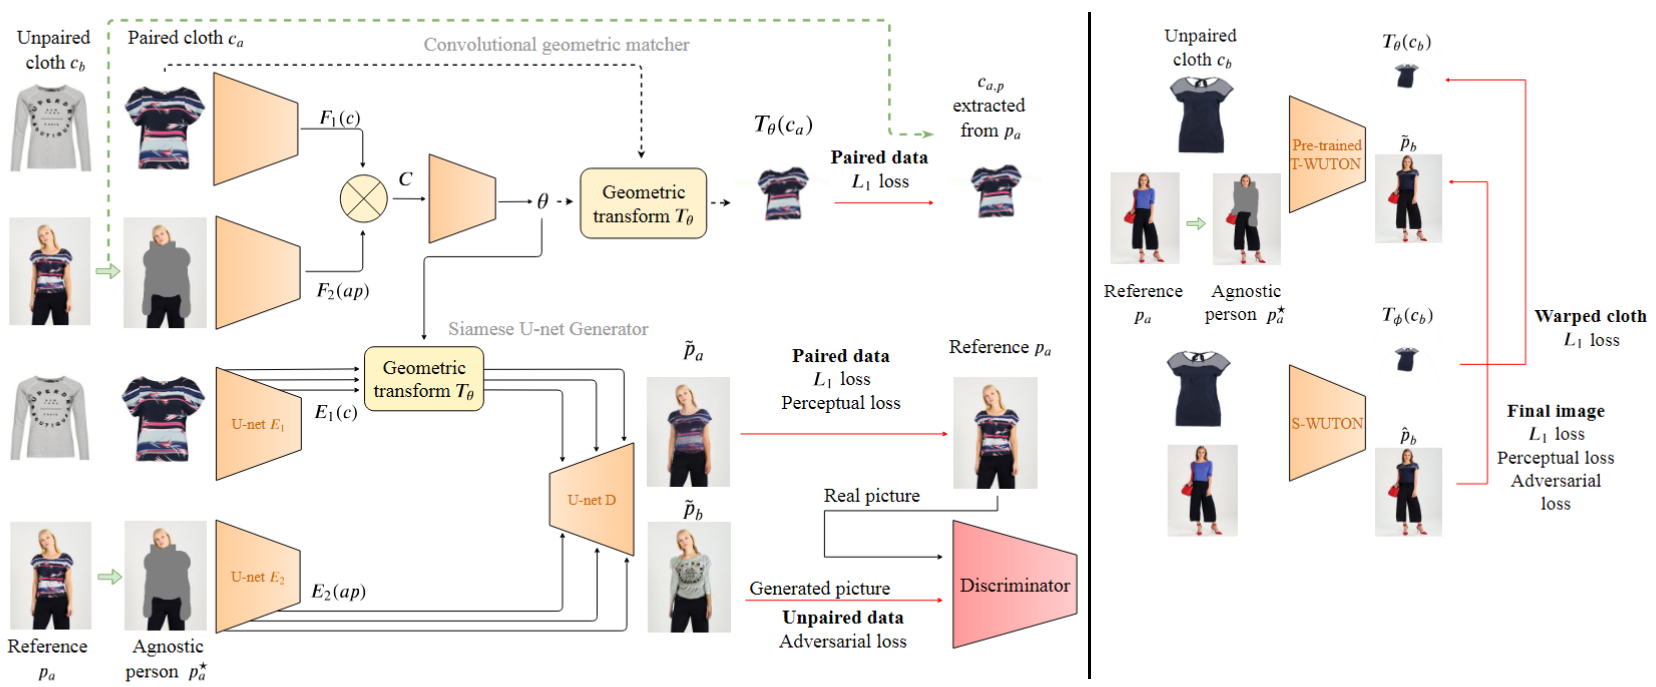
\includegraphics[width=\linewidth]{content/resources/images/literature-review/wuton.png}
    \caption{Overview architecture of WUTON~\cite{Issenhuth-ECCV2020-Do}.}
    \label{fig:vton-wuton}
\end{figure}

WUTON~\cite{Issenhuth-ECCV2020-Do} faces a specific limitation in which the optimization of the Student network is aimed at reconstructing synthetic images produced by the Teacher network. However, the result of the Teacher network has noticeable artifacts, resulting in a decline in the quality of the Student network. Ge et al.~\cite{Ge-CVPR2021-Parser} presented a novel knowledge distillation-based approach (PF-AFN) to overcome this challenge.  In this approach, the parser-free Student network uses the synthetic images generated by a parser-based network as input and learns to reconstruct the original images. By doing so, the training process of the Student network is supervised by real image data. This novel training method has since become the standard for subsequent parser-free methods.

\begin{figure}[h!]
    \centering
    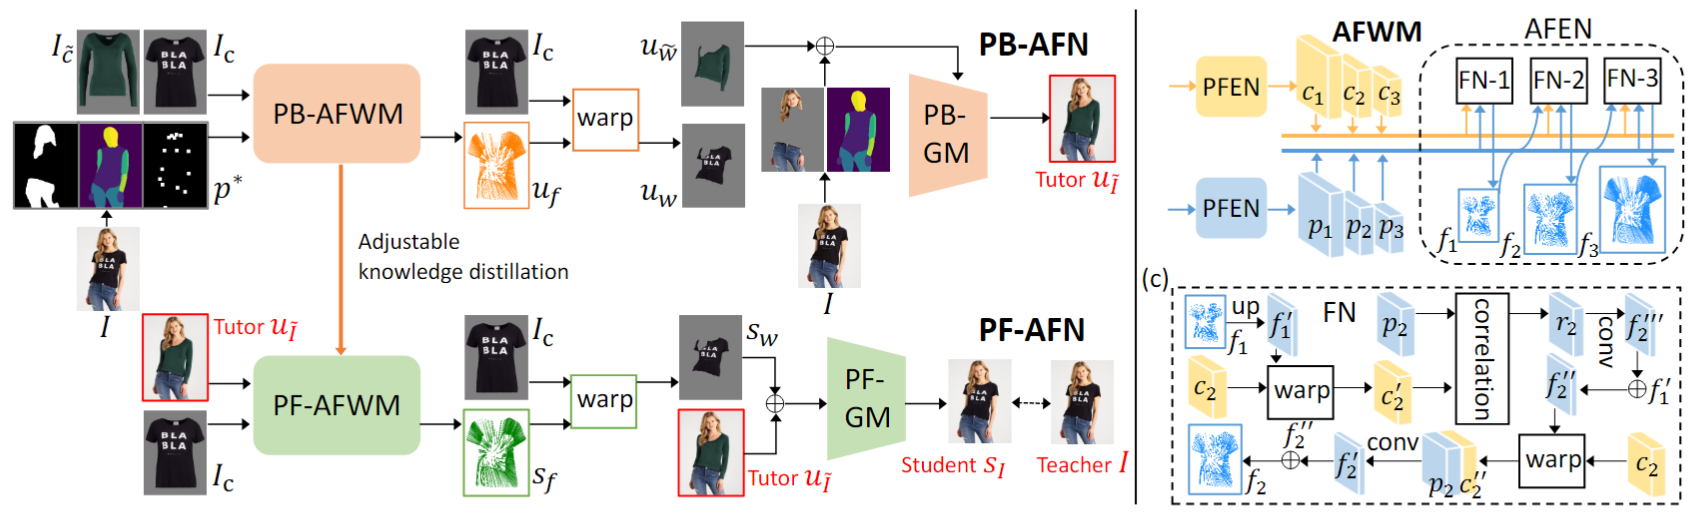
\includegraphics[width=\linewidth]{content/resources/images/literature-review/pfafn.png}
    \caption{Overview architecture of PF-AFN~\cite{Ge-CVPR2021-Parser}.}
    \label{fig:vton-pfafn}
\end{figure}

He et al.~\cite{He-CVPR2022-Style} proposed FS-VTON, an enhanced framework derived from PF-AFN~\cite{Ge-CVPR2021-Parser} with specific improvements in the warping component. The authors introduced a Style-based Global Appearance Flow Estimation using StyleGan blocks~\cite{Karras-CVPR2019-Style}. It enables the model to capture global and local correspondences between clothes and person images, enhancing garment deformation. In contrast, RMGN~\cite{Lin-IJCAI2022-RMGN} directed its focus towards the generation module through the development of a Regional Mask-Guided Generator, built upon SPADE blocks~\cite{Park-CVPR2019-Semantic} and residual connection.

\begin{figure}[h!]
    \centering
    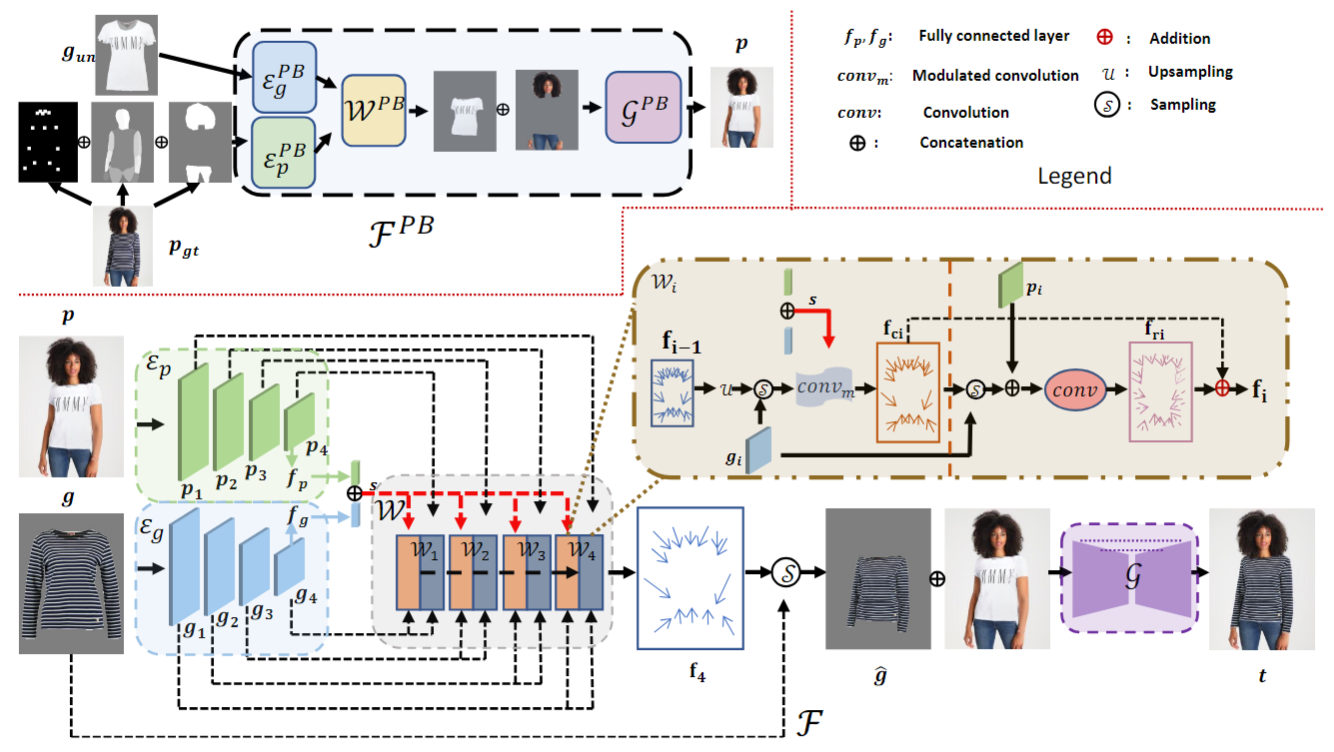
\includegraphics[width=\linewidth]{content/resources/images/literature-review/fsvton.png}
    \caption{Overview architecture of FS-VTON~\cite{He-CVPR2022-Style}.}
    \label{fig:vton-fsvton}
\end{figure}

\begin{figure}[h!]
    \centering
    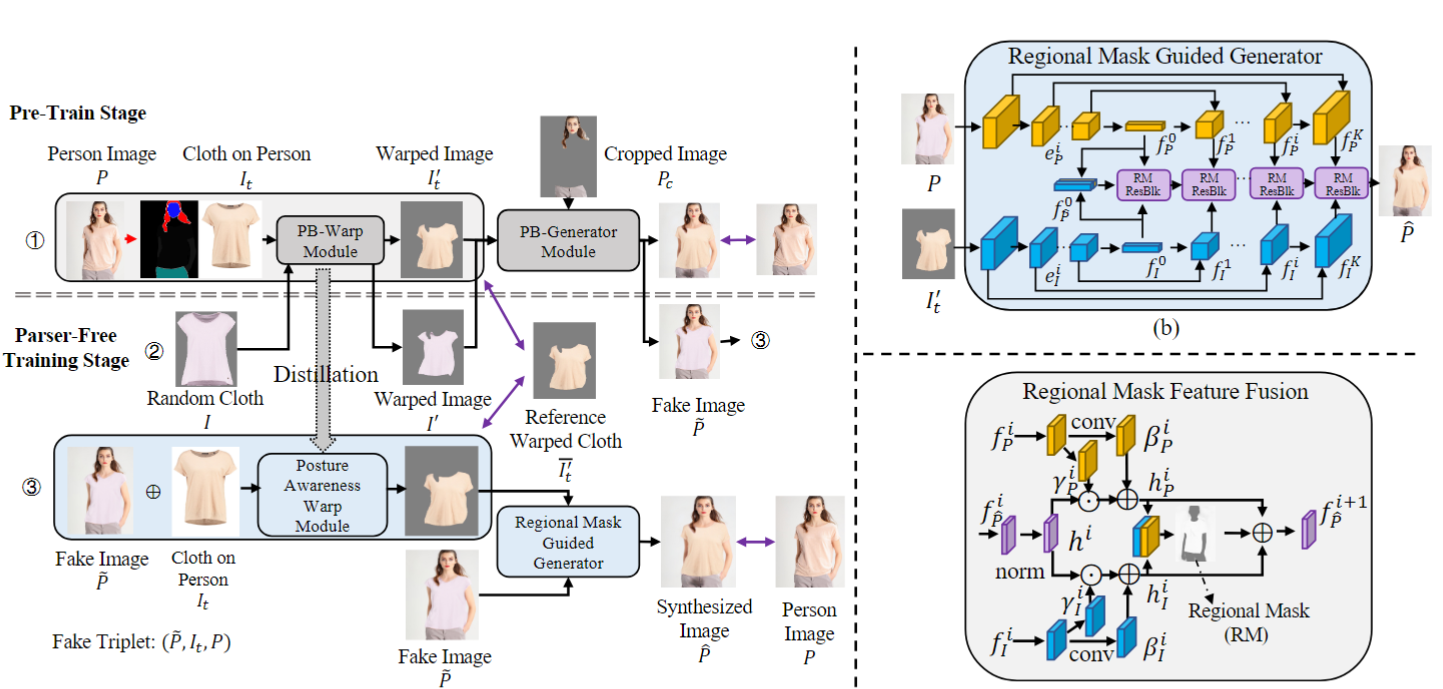
\includegraphics[width=\linewidth]{content/resources/images/literature-review/rmgn.png}
    \caption{Overview architecture of RMGN~\cite{Lin-IJCAI2022-RMGN}.}
    \label{fig:vton-rmgn}
\end{figure}


% \subsection{Video Virtual Try-on}
% \paragraph{Video Virtual Try-on.} There are also methods that aim to perform virtual try-on on a sequence of frames. These methods use techniques like memory-based~\cite{Zhong-ACMMM2021-Mvton} or optical flow~\cite{Kuppa-WACV2021-ShineOn} to keep the temporary consistency between the frames. However, these methods are still based on the parser-based approach, which takes considerable time to calculate the human representation. 

In this thesis, we adopt the parser-free approach to prioritize speed, as calculating human representation is a time bottleneck in the try-on process. However, we take a distinct step from existing methods by modifying the Student network for improved speed and reduced memory consumption while keeping the parser-based approach in the Teacher network to preserve the output quality.

\subsection{Commercial Products}
Companies are experiencing significant advancements in virtual try-on, offering many competitive advantages. Artificial intelligence (AI) and/or augmented reality (AR) are the technologies behind this technology. Such products are not limited to online platforms; even offline store owners can set up on-site kiosks or virtual mirrors,  enabling customers to try on items without risking damage to the actual product. In this part, we explore several commercial products already used by companies.

One example of a virtual try-on product is the virtual try-on for fashion accessories, exemplified by Warby Parker's pioneering initiative to provide customers with a virtual eyewear try-on experience~\cite{WarbyParker-Glasses}. Offering this feature on their website allows customers to experiment with different glasses styles before purchasing. This demand becomes even more important for high-end and costly products. Recognizing this, Baume \& Mercier, a luxury watch company, has enhanced their digital sales experience by incorporating a virtual try-on system~\cite{BaumeMercierr-TimeTide-Watch}.  Their method involves creating 3D watch models in various wrist sizes and striving to replicate transparency and lighting effects accurately~\cite{BaumeMercierr-Hapticmedia-Watch}.

\begin{figure}[h!]
    \centering
    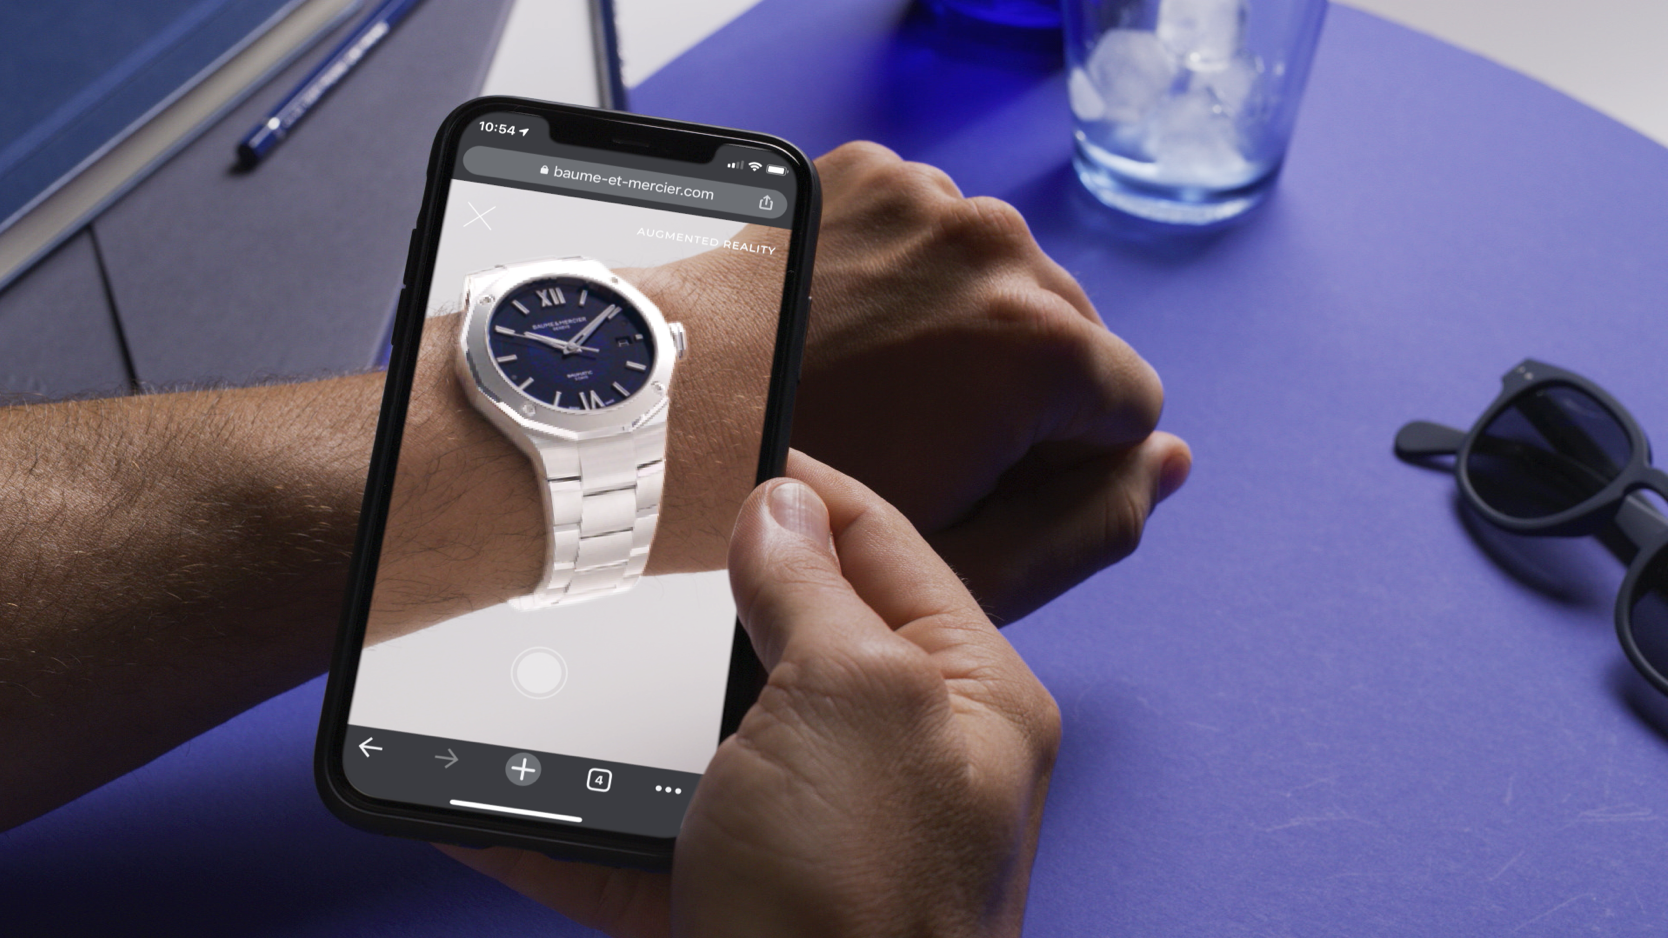
\includegraphics[width=\linewidth]{content/resources/images/literature-review/baume-mercier.png}
    \caption{Virtual try-on with 3D watch models (Source: Baume \& Mercier Virtual Try-On System ~\cite{BaumeMercierr-TimeTide-Watch}).}
    \label{fig:commercial-baume}
\end{figure}

Another awesome application is the virtual try-on for shoes, which leverages AR technologies to visualize how shoes appear on the user's feet. Some of the products that can be mentioned are Amazon virtual try-on for shoes~\cite{AmazonVTO-Aboutamazon2022-Shoes} and Artlabs~\cite{Artlabs-Shoes}, which can fit 3D shoe models onto the customer's feet. Consequently, customers can assess the appearance of the shoes from multiple angles by moving their feet.

The virtual try-on for clothes is another challenge. The methods employed in this domain aim to fit the clothes to suit the target human pose. Compared to the 3D-based solutions, which wear the 3D model of the item to the customer's body~\cite{GeeneeVTO-Clothes} or allow users to create 3D models that represent them to try on~\cite{ZalandoVTO-Zalando2023-Clothes}, the 2d-based virtual try-on product (e.g. Google Shopping virtual try-on~\cite{GoogleVTO-GoogleBlog2023-Clothes}), which use the real models and direct processing on the image, is intensively developing and applying over the years. However, Google Shopping's virtual try-on feature~\cite{GoogleVTO-GoogleBlog2023-Clothes} only allows users to select from the available model images, which makes it difficult for customers who wish to evaluate the fit of items on their bodies.

\begin{figure}[h!]
    \centering
    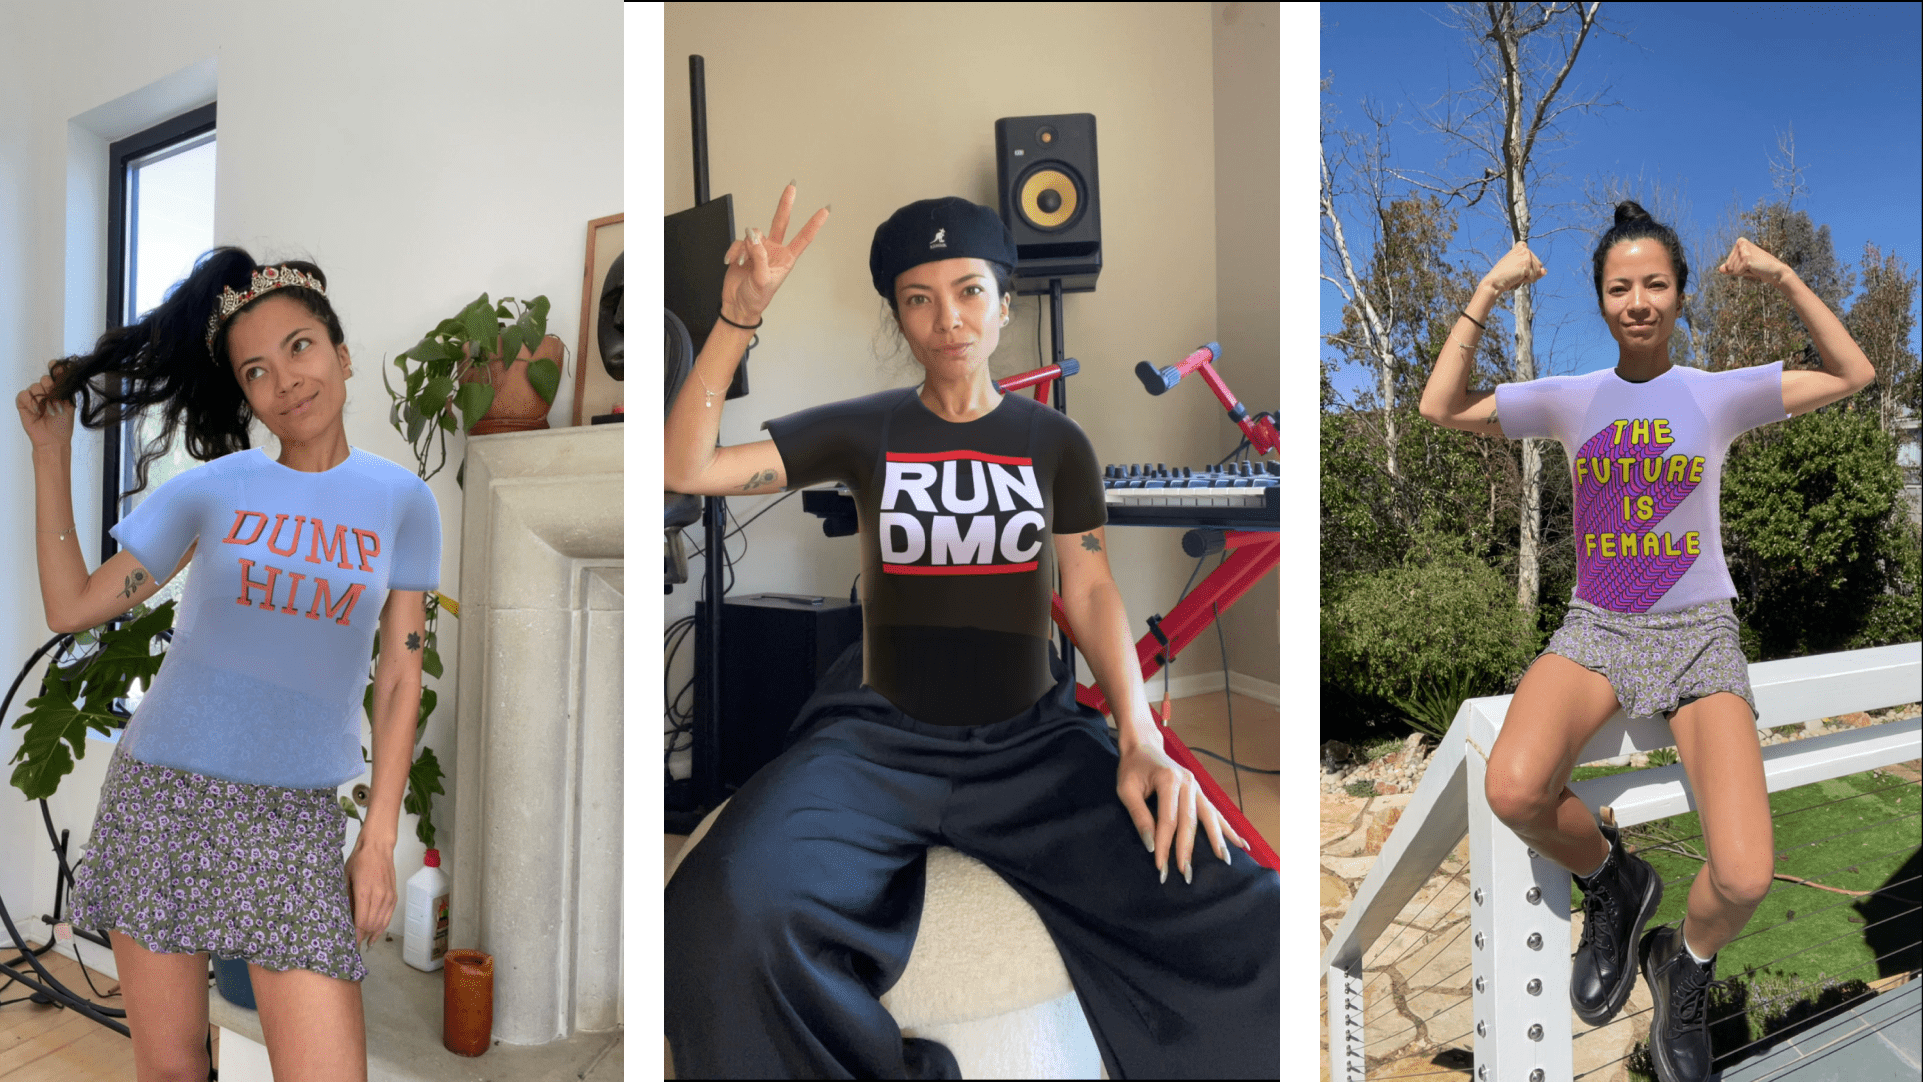
\includegraphics[width=\linewidth]{content/resources/images/literature-review/geenee-ar.png}
    \caption{Tracking human body to wear 3D clothes models (Source: Geenee AR~\cite{GeeneeVTO-Clothes}).}
    \label{fig:commercial-amazon}
\end{figure}

\begin{figure}[h!]
    \centering
    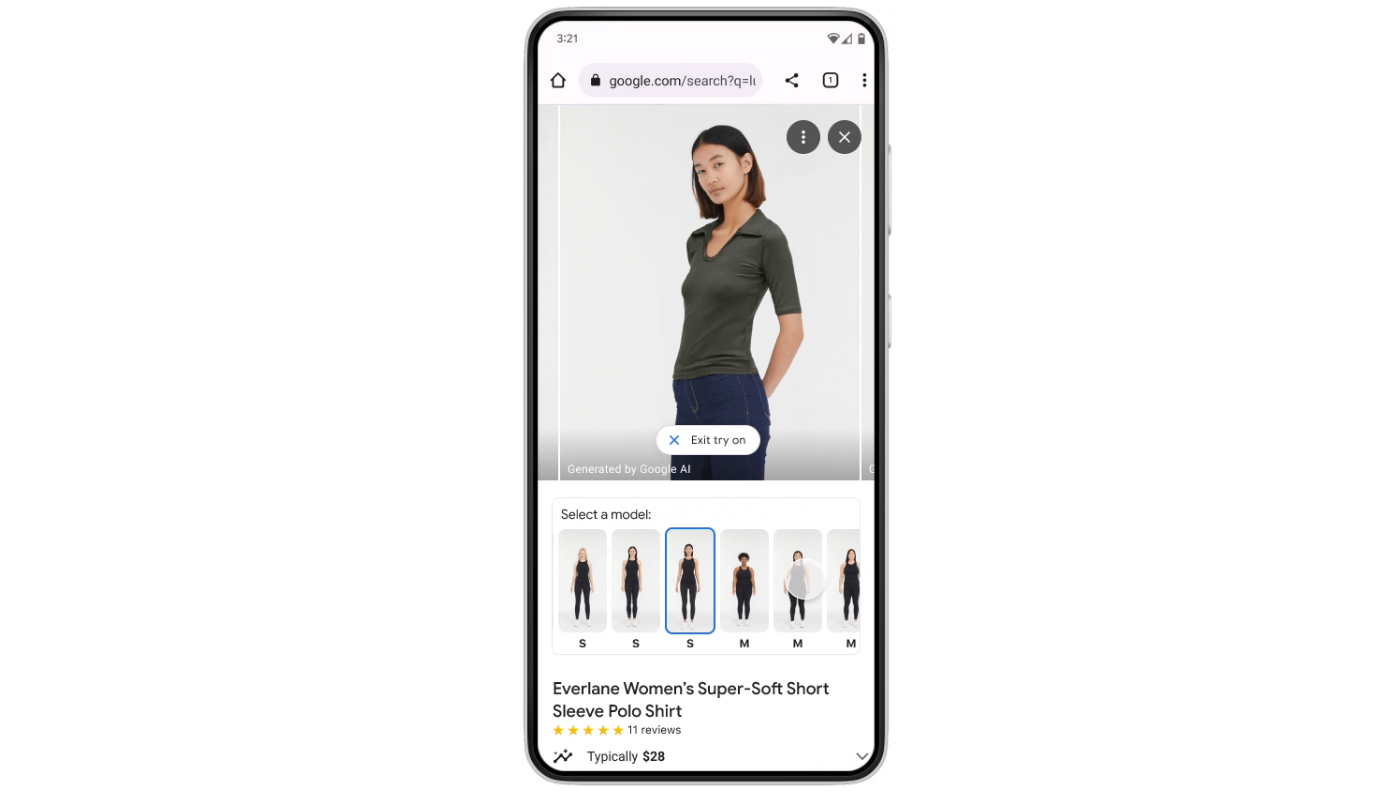
\includegraphics[width=\linewidth]{content/resources/images/literature-review/google-tryon.png}
    \caption{Google AI virtual try-on feature for shopping (Source: Google introduces new AI virtual try-on feature~\cite{GoogleVTO-GoogleBlog2023-Clothes}).}
    \label{fig:commercial-google}
\end{figure}

% Within the scope of this thesis, we focus on how virtually try-on clothes, specifically upper-body clothes. 

 %%%%%%%%%%%%%%%%%%%%%%%%%%%%%%%%%%%%%%%%%%%%%%%%%%%%%%%%%%%%%%%%
 \newpage
\section{Fashion Recommendation}
With the explosion of data and deep learning, a growing number of studies have focused on visual-based fashion recommendations. 
In 2018, Mariya et al.~\cite{Mariya-ECCV18-Learning} provided the PolyvoreOutfits dataset to support the fill-in-the-blank task, where we need to find an item of a specific category to complete a partial outfit. 
\begin{figure}[h!]
    \centering
    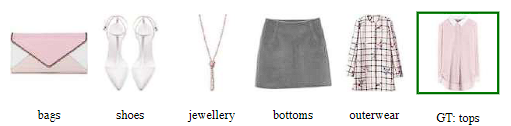
\includegraphics[width=0.6\linewidth]{content/resources/images/literature-review/fitb.PNG}
    \caption{Outfit fill-in-the-blank task, where the highlighted item is the missing item (Source: Fashion Outfit Complementary Item Retrieval~\cite{Lin-CVPR2020-Fashion}).}
    \label{fig:fitb-task}
\end{figure}

They also propose a Type-Aware network (\autoref{fig:type-aware}) as the baseline framework. 
Initially, the framework learns a shared embedding space where all fashion items are represented. Subsequently, this shared embedding space is projected into subspaces based on pairs of item types. For example, in the top-shoes subspace, the shoes that match a specific top must be close, even if they differ significantly in the overall embedding space.

\begin{figure}[h!]
    \centering
    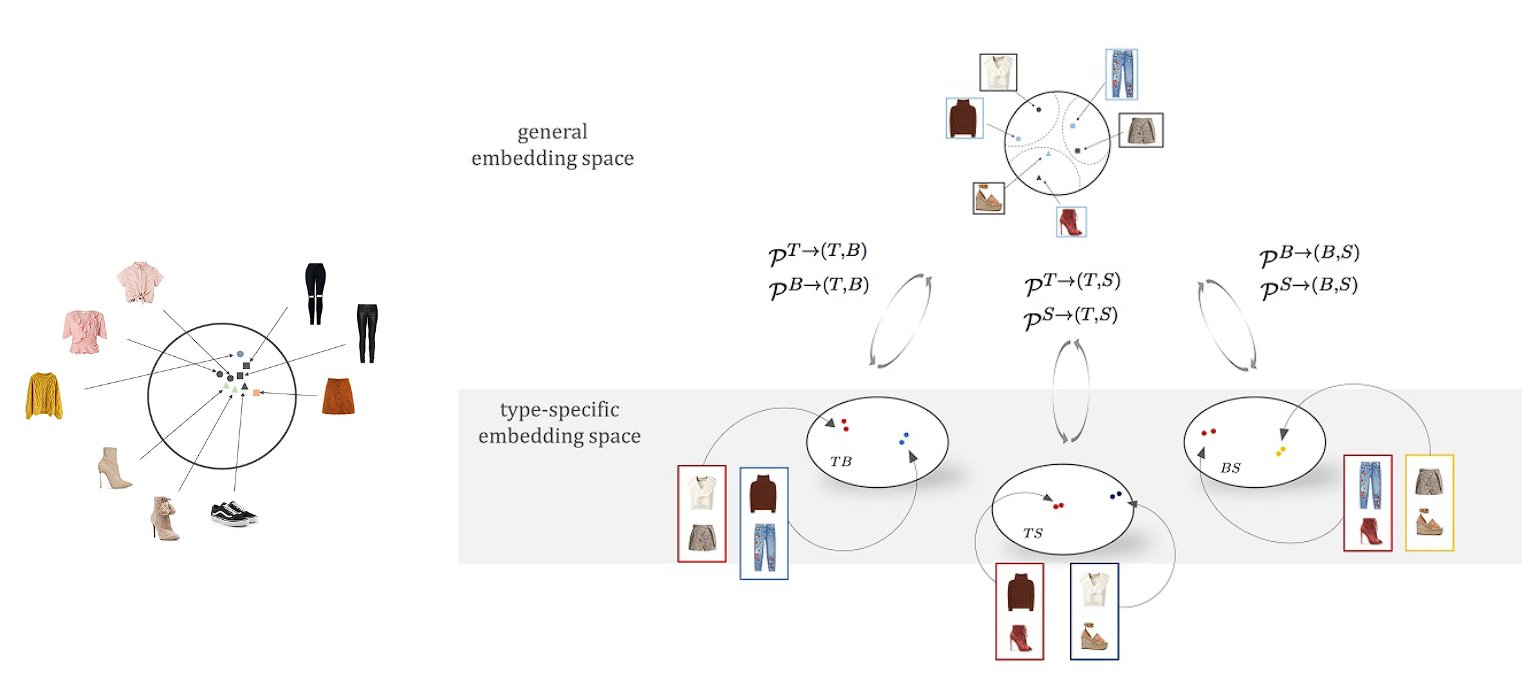
\includegraphics[width=\linewidth]{content/resources/images/literature-review/TypeAware.PNG}
    \caption{Type-Aware learning strategies (Source: Learning Type-Aware Embeddings for Fashion
Compatibility~\cite{Mariya-ECCV18-Learning}).}
    \label{fig:type-aware}
\end{figure}

After the Self-Attention mechanism and Transformers architecture \cite{Vaswani-NeurIPS2017-Attention} were introduced and gained success in the natural language processing task~\cite{Devlin-ArXiv2018-BERT}, CSA-Net~\cite{Lin-CVPR2020-Fashion} and OutfitTransformer~\cite{Sarkar-CVPRW2022-OutfitTransformer} incorporated these ideas by utilizing the textual embeddings of the categories and significantly improved the recommendation results. 

\begin{figure}[h!]
    \centering
    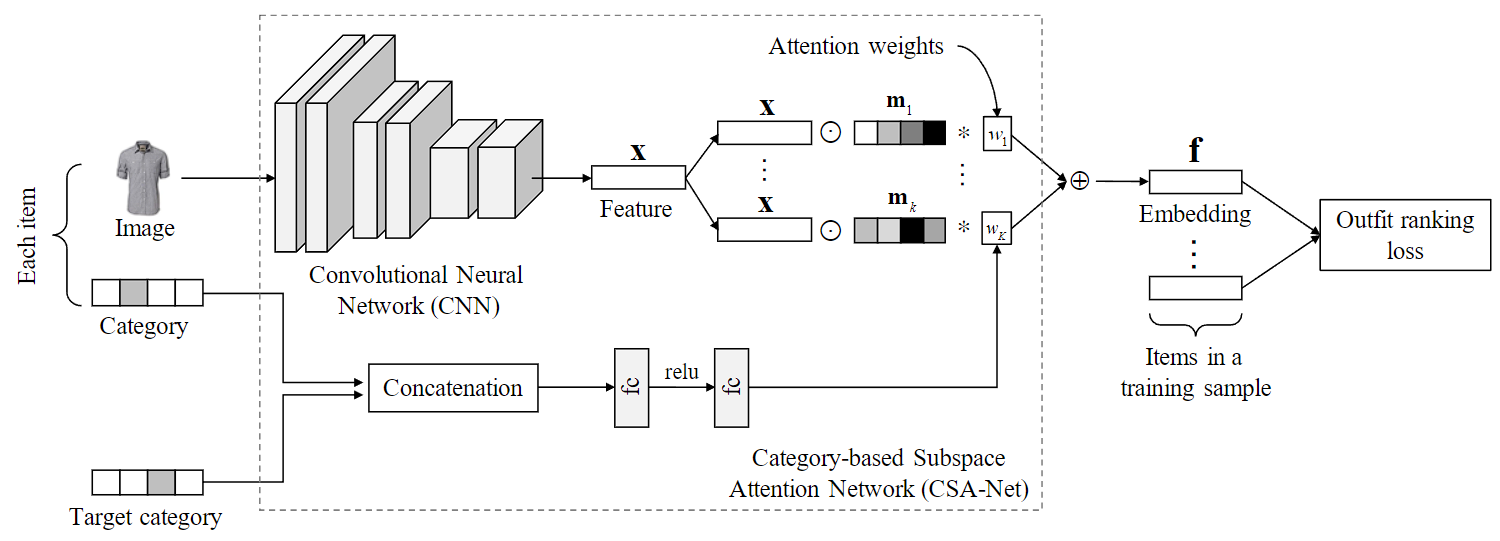
\includegraphics[width=\linewidth]{content/resources/images/literature-review/CSA.PNG}
    \caption{Overview of CSA-Net framework (Source: Fashion Outfit Complementary Item Retrieval~\cite{Lin-CVPR2020-Fashion}).}
    \label{fig:csa}
\end{figure}

Specifically, CSA-Net represents each category by an embedding vector to capture their textual semantics. The CSA-Net framework (illustrated in \autoref{fig:csa}) takes a reference image, its category vector, and a target category vector. A Convolution Neural Network is employed to extract the image embedding. This vector is then multiplied by a set of masks to create multiple subspace embeddings (multi-attention head). The concatenated category vector is used to predict the attention weights, which determine the contribution of each subspace embeddings in the final output embedding.

To eliminate the learning of pair-wise embeddings in the above methods, OutfitTransformer~\cite{Sarkar-CVPRW2022-OutfitTransformer} learns the embedding of an entire outfit by utilizing the Transformer Encoder block and a special token at the first position (same as \textit{<CLS>} token in BERT~\cite{Devlin-ArXiv2018-BERT}). This token not only captures the embeddings of all items in the outfit but also specifies the target category for the missing item (as shown in \autoref{fig:outfittransformer}).

\begin{figure}[h!]
    \centering
    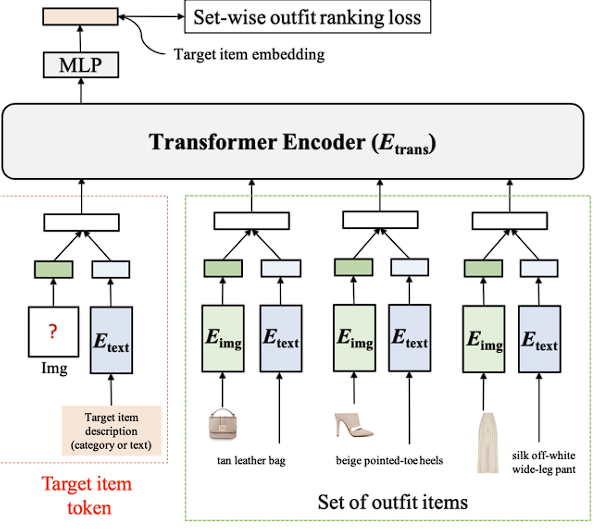
\includegraphics[width=0.6\linewidth]{content/resources/images/literature-review/OutfitTransformers.PNG}
    \caption{Overview of OutfitTransformer framework (Source: OutfitTransformer: Outfit Representations for Fashion Recommendation~\cite{Sarkar-CVPRW2022-OutfitTransformer}).}
    \label{fig:outfittransformer}
\end{figure}

Wu et al.~\cite{Wu-CVPR2021-FashionIQ} further expanded the research scope by introducing the FashionIQ dataset for the text feedback-guided item retrieval task, where we need to find the desired item given a reference input item and its relative attribute feedback in the natural language. \autoref{fig:fashioniq} demonstrates the retrieval pipeline based on the user's feedback.

\begin{figure}[h!]
    \centering
    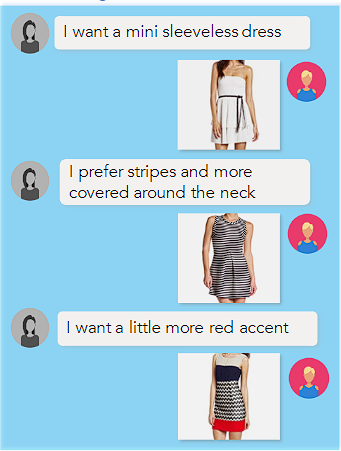
\includegraphics[width=0.4\linewidth]{content/resources/images/literature-review/fashioniq.PNG}
    \caption{Demonstration of feedback-guided retrieval (Source: Fashion IQ: A New Dataset Towards Retrieving Images by Natural Language Feedback~\cite{Wu-CVPR2021-FashionIQ}).}
    \label{fig:fashioniq}
\end{figure}

By utilizing CLIP~\cite{Radford-OpenAIblog2019-Language}, a deep learning model that learns the joint representations of both images and textual descriptions, Baldrati et al. \cite{Baldrati-CVPR2022-Effective, Baldrati-CVPR2022-Conditioned} achieved state-of-the-art performance on the FashionIQ dataset, proving its applicability to the fashion domain for text feedback-guided image retrieval. 

\begin{figure}[h!]
    \centering
    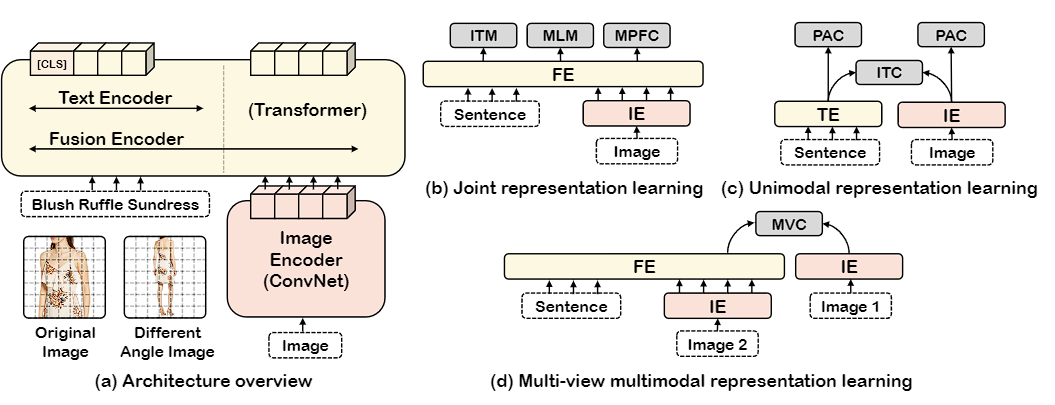
\includegraphics[width=\linewidth]{content/resources/images/literature-review/fashionvil.PNG}
    \caption{Overview of FashionViL architecture (Source: FashionViL: Fashion-Focused
Vision-and-Language Representation Learning~\cite{Han-ECCV2022-FashionViL}).}
    \label{fig:fashionvil}
\end{figure}

Han et al.~\cite{Han-ECCV2022-FashionViL} bridged the gap between the text feedback-guided image retrieval problem and the fill-in-the-blank problem by proposing a general vision-and-language network framework. The FashionViL overall architecture is shown in~\autoref{fig:fashionvil}. The framework optimizes its text and image encoders by learning multiple tasks such as Multi-view contrastive learning (MVC), Pseudo-attribute classification (PAC), Masked patch feature classification (MPFC), Image-text contrastive learning (ITC), Image-text matching (ITM), and Masked language modelling (MLM). Subsequently, the framework encoders can produce universal embeddings for downstream tasks such as text feedback-guided image retrieval or fill-in-the-blank problem.
 %%%%%%%%%%%%%%%%%%%%%%%%%%%%%%%%%%%%%%%%%%%%%%%%%%%%%%%%%%%%%%%%
\section{Similarity Search}
Similarity search has become a hot topic in recent years due to the explosion of data. There are two main types of similarity search: exhaustive and approximate. Exhaustive searching, such as the K-Nearest Neighbor (KNN) algorithm, involves calculating the distances between the query point and all items in a dataset to find the nearest neighbours. This approach provides accurate results but can be computationally expensive, especially in large datasets or high dimensional data points.

Approximate searching rises as the solution for the time complexity of exhaustive searching. These methods either reduce the dataset dimension or limit the search scope with the trade-off for accuracy. Production Quantization (PQ)~\cite{Jegou-TPAMI2010-Product} clusters each dimension or group of dimensions into buckets and indexes the dataset by those buckets instead, thus reducing the number of bytes required to represent the dataset (as illustrated in \autoref{fig:product-quantization}).

\begin{figure}[h!]
    \centering
    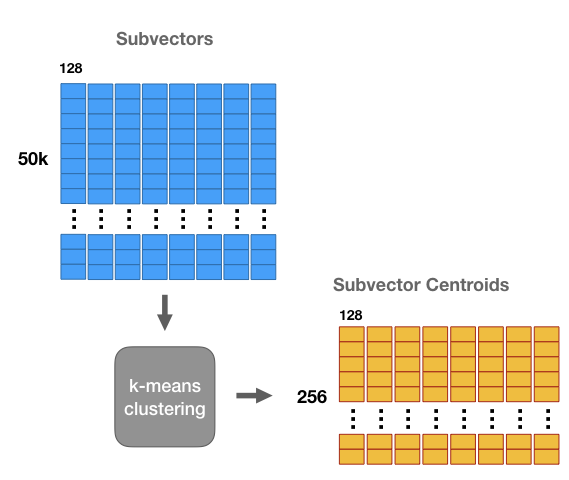
\includegraphics[width=0.6\linewidth]{content/resources/images/literature-review/kmeans_clustering.png}
    \caption{Overview of Production Quantization method (Source: Product Quantizers for k-NN Tutorial Part 1~\cite{web-pq}).}
    \label{fig:product-quantization}
\end{figure}

In terms of limiting the search scope, Inverted File Index (IVF)~\cite{Sivic-ICCV2003-Video} divides the search space into subspaces and only searches in a subset of these subspaces. Some methods leverage the tree~\cite{Erik-Github-Annoy} or graph~\cite{Malkov-TPAMI2018-Efficient} data structure to speed up the search process with the cost of more memory consumption. Specifically, Hierarchical Navigable Small Worlds~\cite{Malkov-TPAMI2018-Efficient} constructs multiple subgraphs from all items; the lower the level is, the denser the subgraph becomes, and the searching process is performed like in a Skip List. Approximate Nearest Neighbors Oh Yeah~\cite{Erik-Github-Annoy} builds a binary tree by repeatedly choosing two random items and splitting the space into two subspaces; Spotify's recommendation system uses this algorithm.
\chapter{Virtual Try-on}
\label{chapter-virtual-tryon}
\begin{ChapAbstract}
In this chapter, we propose Distilled Mobile Real-time Virtual Try-On (DM-VTON), which focuses on synthesizing try-on images with increased speed compared to previous methods while ensuring accuracy. Our approach is based on a knowledge distillation scheme that leverages a strong Teacher network as supervision to guide a Student network without relying on human parsing. Notably, we introduce an efficient Mobile Generative Module within the Student network, significantly reducing the runtime while ensuring high-quality output. Additionally, we propose Virtual Try-on-guided Pose for Data Synthesis to address the limited pose variation observed in training images. Finally, we provide the experimental details of our proposed method, and then we present a comparative study of DM-VTON with state-of-the-art methods.
\end{ChapAbstract}

%%%%%%%%%%%%%%%%%%%%%%%%%%%%%%%%%%%%%%%%%%%%%%%%%%%%%%%%%%%%%%%%
\section{Overview}
\begin{figure}[h!]
  \centering
  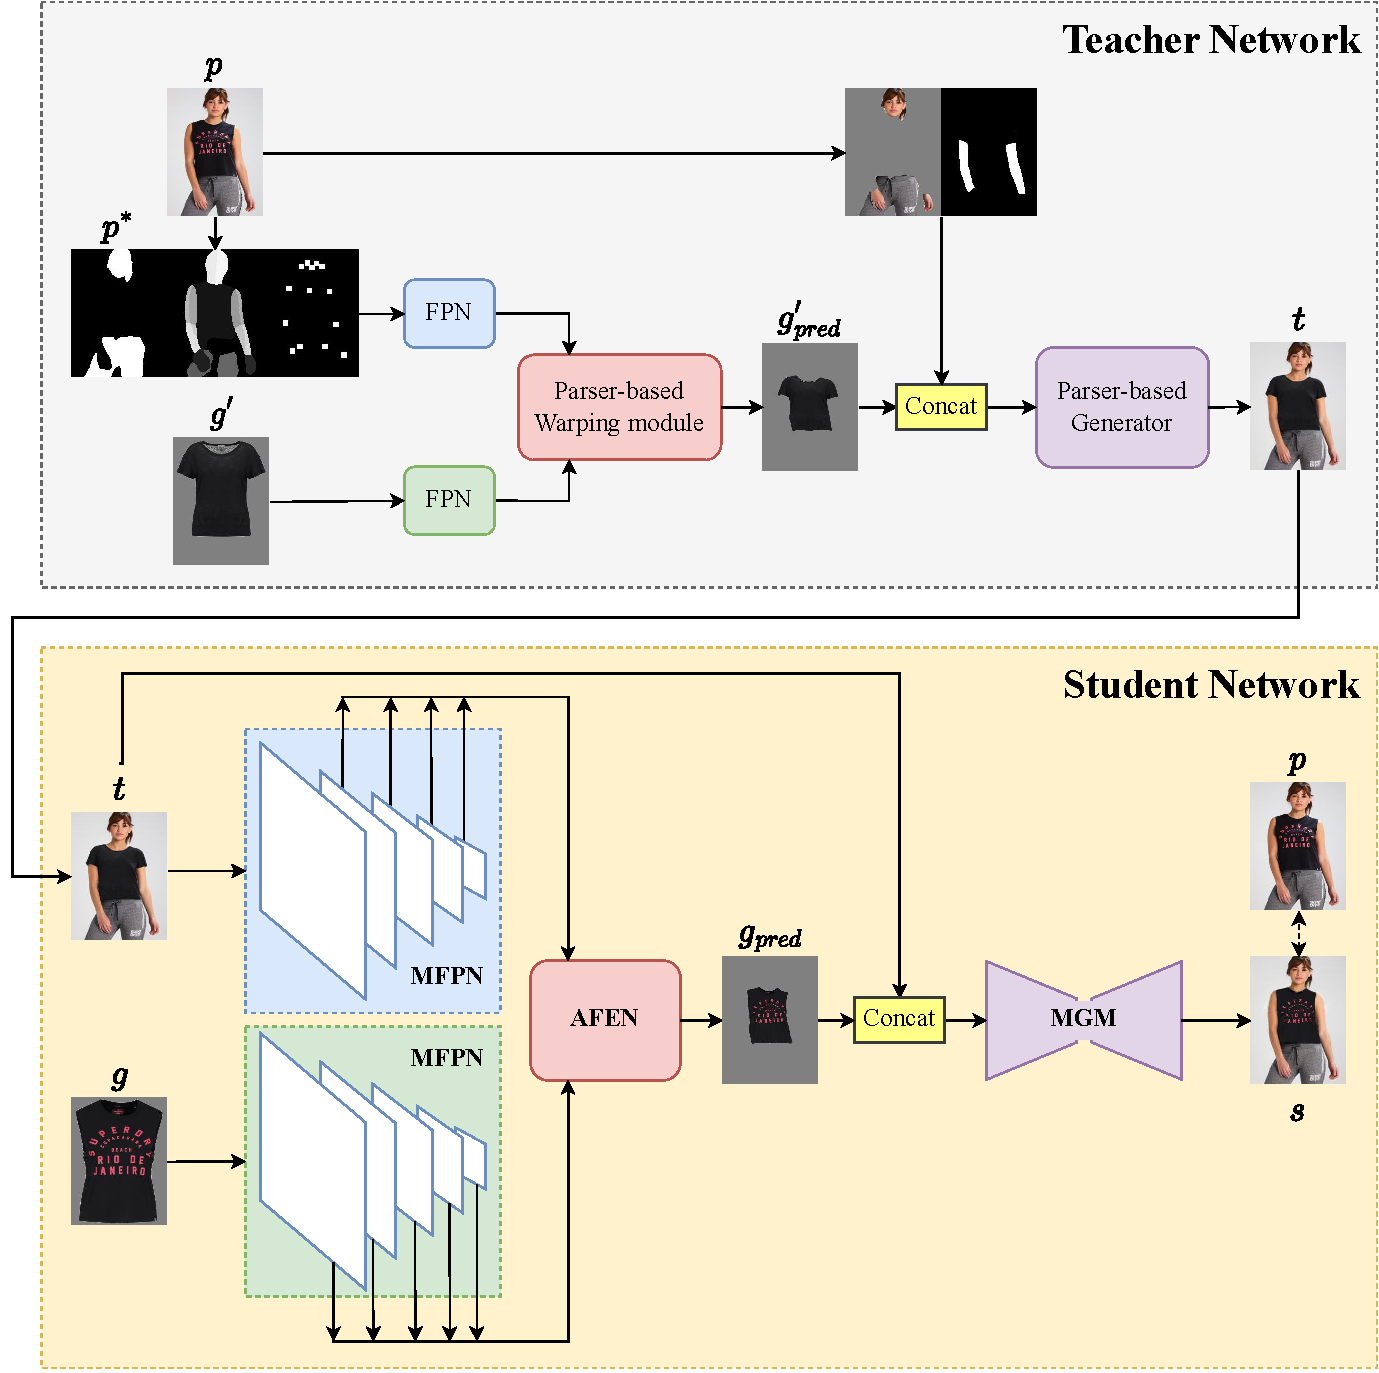
\includegraphics[width=\textwidth]{content/resources/images/tryon/mobile-tryon.pdf}
  \caption{Overview architecture of the proposed Distilled Mobile Real-time Virtual Try-On (DM-VTON) framework. The parser-based Teacher network generates a synthetic image as the input for training the Student network.}
  \label{fig:mobile-tryon}
  \vspace{-1mm}
\end{figure}

Our objective is to generate an image of a person wearing a specific garment while preserving the rest of the image. To achieve this goal, we adopt the knowledge distillation training pipeline~\cite{Hinton-Arxiv2015-Distilling, Issenhuth-ECCV2020-Do, Ge-CVPR2021-Parser, He-CVPR2022-Style, Lin-IJCAI2022-RMGN} to develop a Distilled Mobile Real-time Virtual Try-On (DM-VTON) framework (see~\autoref{fig:mobile-tryon}). Our proposed DM-VTON consists of two networks: Teacher and Student networks. Both include several main components: feature extractor, clothes-warping module, and generator. 


The Teacher network aims to produce the virtual try-on result using the parser-based training process. The Student network then utilizes the Teacher network to generate synthetic input images, enabling the Student network to be supervised by the original images without relying on human representation. The Teacher network is built upon SOTA virtual try-on models to ensure high-quality output. Focusing on inference speed, we propose lightweight components for the Student network. 

%%%%%%%%%%%%%%%%%%%%%%%%%%%%%% 
\section{Appearance Flow}
The concept of appearance flow begins with a method for synthesizing images of the same object observed from arbitrary viewpoints introduced by Zhou et al.~\cite{Zhou-ECCV2016-AppearanceFlow}. From the observation that the appearance (texture, shape, colour, etc.) of different views of an object are highly correlated, research suggests that the information of an input view can be used to generate images for various views. Appearance flow refers to 2-D coordinate vectors specifying which pixels in the input view could be used to synthesize the target view. Specifically, with the pixel $i$ of the target image, the appearance flow vector $f^i \in \mathbb{R}^2$ indicates the coordinate of the input pixel sampled to reconstruct it (as illustrated in~\autoref{fig:appearance-flow-ex}). This idea is also applied to solve many problems, such as visual tracking~\cite{Song-ICCV2017-Crest}, pose transfer~\cite{Li-CVPR2019-Dense}, image inpainting~\cite{Liu-ECCV2020-Rethinking}, virtual try-on~\cite{Ge-CVPR2021-Parser, He-CVPR2022-Style}

\begin{figure}[h]
    \centering
    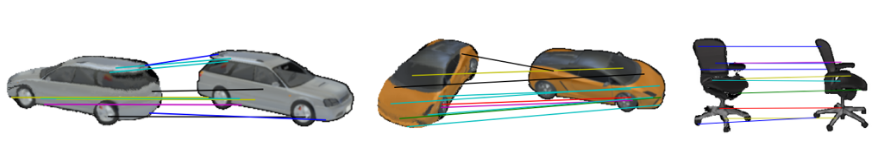
\includegraphics[width=\linewidth]{content/resources/images/tryon/appearance-flow-ex.png}
    \caption{Illustration of appearance flow vectors (Source: View Synthesis by Appearance Flow~\cite{Zhou-ECCV2016-AppearanceFlow}).}
    \label{fig:appearance-flow-ex}
\end{figure}

%%%%%%%%%%%%%%%%%%%%%%%%%%%%%% 
\section{Teacher Network}

The main purpose of this network is to generate a synthetic person image that serves as the input for the Student training process. Furthermore, the Teacher also helps this process through a knowledge distillation scheme. In particular, we take advantage of the SOTA method of virtual try-on task: FS-VTON \cite{He-CVPR2022-Style}. As shown in~\autoref{fig:mobile-tryon}, it incorporates two feature pyramid networks (FPN)~\cite{Lin-CVPR2017-FPN} constructed from residual blocks, enabling the extraction of features from the human representation $p^*$ and garment image $g'$. To achieve the garment deformation functionality, the Teacher network utilizes a style-based global appearance flow estimation network that uses modulated convolution \cite{Karras-CVPR2019-Style}. This network first predicts a coarse appearance flow via extracted global style vector and then refines it locally. The last flow thus can capture the global and local correspondence between the garment and the target person. This makes the Teacher network more robust against the problems of detail-preserving and large misalignment. Finally, the warped clothes and the preserved region on the human body are concatenated as the generator input for try-on result generation. The generator of our Teacher network follows the encoder-decoder architecture with skip connections, which have been proven effective in detail preservation.

Because the inputs of the parser-based model (i.e., human representation) contain more semantic information when compared to those in the parser-free model, we employ an adjustable knowledge distillation learning scheme~\cite{Ge-CVPR2021-Parser} with a distillation loss to guide the Student network. When training the Student network with fake image $t$ and garment $g$, we also pass $p*$ and $g$ through the pretrained Teacher network. The distillation loss is formulated as follows:
\begin{align}
    L_{dis}  & = \lambda_{fea}L_{fea} + \lambda_{flow}L_{flow},\\
    L_{fea}  & = \psi \sum_{i=1}^N(p^{pb}_{i} - t^{pf}_{i})^2 + \psi \sum_{i=1}^N(g^{pb}_{i} - g^{pf}_{i})^2,\\
    L_{flow} & = \psi \sum_{i=1}^N\|f^{pb}_{i} - f^{pf}_{i}\|_{2},\\
    \psi     & = \{\begin{array}{l} 1, ~if~ \|t-p\|_1<\|s-p\|_1 \\ 0,~otherwise \end{array},
\end{align}
where $t$, and $s$ are the try-on result of the Teacher and Student, respectively; $p$ is the person image ground truth. $p^{pb}_{i}$ and $t^{pf}_{i}$ denote the output feature maps at the $i$-th scale extracted from $p*$ and fake image $t$; similarly, $g^{pb}_{i}$ and $g^{pf}_{i}$ are the $i$-th scale feature maps extracted from garment image $g$ by the feature extractor of parser-based and parser-free network, respectively. $f^{pb}_{i}$ and $f^{pf}_{i}$ are the predicted appearance flows from the Teacher and Student warping modules at the $i$-th scale. $\psi$ is the adjustable factor used to adjust so that the distilling process takes place only if the quality of the generated image of the parser-based network is better than that of the parser-free network.

%%%%%%%%%%%%%%%%%%%%%%%%%%%%%% 
\section{Student Network}

We propose a parser-based approach for synthesizing try-on images with increased speed compared to previous methods while ensuring accuracy. As shown in~\autoref{fig:mobile-tryon}, our Student network consists of three key components: Mobile Feature Pyramid Network (MFPN), Appearance Flow Estimation Network (AFEN), and Mobile Generative Module (MGM). These components synergistically collaborate to extract features, manipulate garments through deformation, and generate try-on images. The AFEN introduced by Ge et al.~\cite{Ge-CVPR2021-Parser} proved effective in deforming garments by using appearance flow estimates from pyramid features. The MFPN and MGM are built upon the architecture of MobileNetV2~\cite{Sandler-CVPR2018-Mobilenetv2} with Inverted Residual blocks specifically designed to optimize computational efficiency and model size.

%%%%%%%%%%%%%%%%%%%%%%%%%%%%%% 
\subsection{Mobile Feature Pyramid Network}
% \footnote{https://github.com/libiseller/MobileNetV2-dynamicFPN}
As shown in~\autoref{fig:mobile-pyramid}, MFPN incorporates the architecture of MobileNetV2 with Inverted Residual blocks~\cite{Sandler-CVPR2018-Mobilenetv2} to a Feature Pyramid Network. By leveraging the capabilities of two MFPN blocks, we extract two-branch N-level feature maps from person and garment images within a parser-free network. These features are fed into the Appearance Flow Estimation Network (AFEN) to predict the appearance flow map for garment deformation.

\begin{figure}[h!]
  \centering
  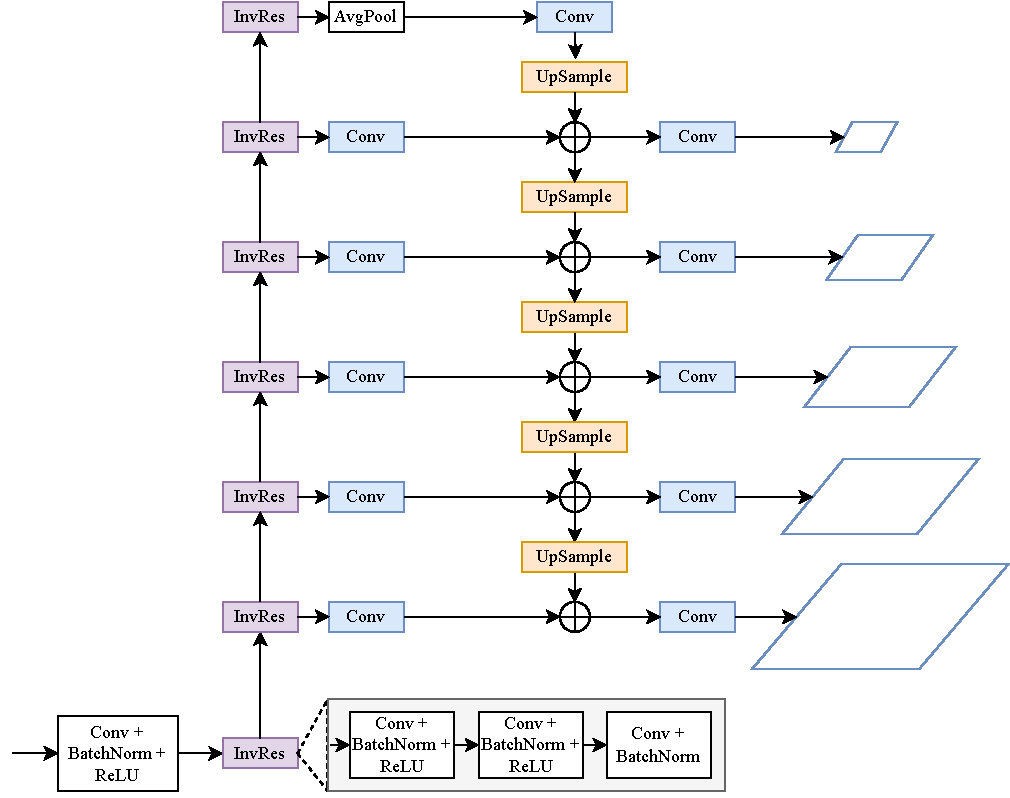
\includegraphics[width=\linewidth]{content/resources/images/tryon/mobile-pyramid.pdf}
  \caption{Mobile Feature Pyramid Network architecture}
  \label{fig:mobile-pyramid}
  \vspace{-2mm}
\end{figure}

%%%%%%%%%%%%%%%%%%%%%%%%%%%%%% 
\subsection{Appearance Flow Estimation Network}
This component aims to deform the garment to fit the human pose while preserving the texture. Following the work of Ge et al.~\cite{Ge-CVPR2021-Parser}, we adopt an appearance flow estimation network (AFEN) comprising subnetworks equipped with varying sizes of convolution layers. These subnetworks are responsible for estimating flows based on extracted multi-level feature maps. The outcome of this network can capture the long-range correspondence between the garment image and the person image, effectively minimizing issues related to misalignment. To enhance the preservation of clothing characteristics, this module is optimized with the second-order constraint:
\begin{equation} 
L_{sec}=\sum_{i=1}^N \sum_t \sum_{\pi \in N_t} CharLoss\left(f_i^{t-\pi}+f_i^{t+\pi}-2 f_i^t\right),
\end{equation}
where $f_i^t$ denotes the $t$-th point on the $i$-th scale flow map; $N_t$ is the set of horizontal, vertical, and diagonal neighborhoods around the $t$-th point; and $CharLoss$ denotes generalized Charbonnier loss~\cite{Sun-IJCV2014-Quantitative}.

%%%%%%%%%%%%%%%%%%%%%%%%%%%%%% 
\subsection{Mobile Generative Module}
To synthesize the entire try-on image from the warped image and target person image, we develop a Mobile Generative Module, the integration of the architectural principles of UNet~\cite{Ronneberger-MICCAI2015-Unet} and MobileNetV2~\cite{Sandler-CVPR2018-Mobilenetv2} as illustrated in~\autoref{fig:mobile-unet}. The primary objective behind the design of this generator is to reduce both the computational burden and the model's overall size.

\begin{figure}[h!]
  \centering
  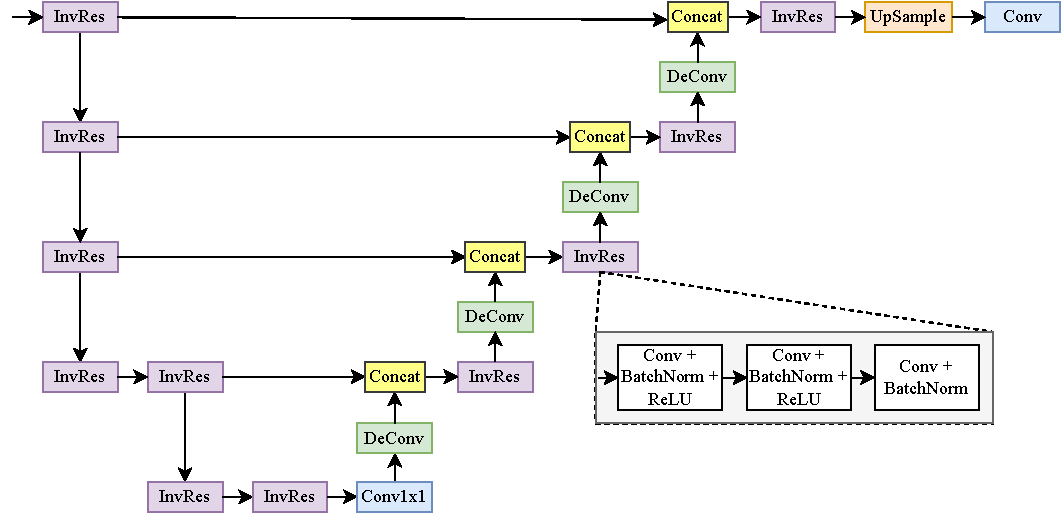
\includegraphics[width=\linewidth]{content/resources/images/tryon/mobile-unet.pdf}
  \caption{Mobile Generative Module architecture}
  \label{fig:mobile-unet}
  \vspace{-2mm}
\end{figure}

%%%%%%%%%%%%%%%%%%%%%%%%%%%%%% 
\subsection{Loss Function}
During training, we optimize the warping module separately in the first stage and then train together with the generator in the last stage. The loss function used in the first stage is defined as:
\begin{align}
    L^{warp} & = \lambda^{warp}_{l}L^{warp}_{l} + \lambda^{warp}_{per}L^{warp}_{per} + \lambda_{sec}L_{sec} + \lambda_{dis}L_{dis},\\
    L^{warp}_{l} & = \|g_{pred} - p \odot m_{gt}\|,\\
    L^{warp}_{per} & = \sum_i{\|\Phi_i(g_{pred}) - \Phi_i(p \odot m_{gt})\|},
\end{align}
where $L^{warp}_{l}$ denotes pixel-wise L1 loss, $L^{warp}_{per}$ is the perceptual loss~\cite{Johnson-ECCV2016-Perceptual}, $L^{warp}_{sec}$ is the smooth loss (second-order constrain), $L^{warp}_{dis}$ is the distillation loss, $g_{pred}$ is warped garment.  $p$ is the person image ground truth with the garment mask $m_{gt}$; $\Phi_i$ denotes the $i$-th block of pre-trained VGG19~\cite{Simonyan-ArXiv2014-VGG}.

With the generative module, we also apply L1 loss perceptual loss~\cite{Johnson-ECCV2016-Perceptual} between the synthesized image and the ground truth image to supervise the training process of MGM:
\begin{align}
    L^{gen} & = \lambda^{gen}_{l}L^{gen}_{l} + \lambda^{gen}_{per}L^{gen}_{per},\\
    L^{gen}_{l} & = \|s - p\|,\\
    L^{gen}_{per} & = \sum_i{\|\Phi_i(s) - \Phi_i(p)\|},
\end{align}
where $L^{gen}_{l}$ is L1 loss and $L^{gen}_{per}$ is the perceptual loss~\cite{Johnson-ECCV2016-Perceptual}. $s$ and $p$ are the generated output of the Student network and the person image ground truth, respectively. 

In practice, we empirically set $\lambda^{warp}_{l}$ = 1, $\lambda^{warp}_{per}$ = 0.2, $L^{warp}_{sec}$ = 6, $L^{warp}_{dis}$ = 0.04, $\lambda^{gen}_{l}$ = 5,
 $\lambda^{gen}_{per}$ = 1. The overall loss function 
when training the whole model in the last stage is:
\begin{align}
    L & = 0.25*L^{warp} + L^{gen}.
\end{align}

\section{Virtual Try-on-guided Pose for Data Synthesis}

By using the K-Means clustering algorithm, we observe that the original VITON dataset~\cite{Han-CVPR2018-Viton} is mainly composed of images with straight-arm poses (as in~\autoref{fig:pose-distribution}(a)). This bias creates a challenge as models trained on such data are prone to overfit and perform poorly on images with different upper-body poses. To tackle this problem, we propose the Virtual Try-on-guided Pose for Data Synthesis (VTP-DS) pipeline. Intending to improve the existing virtual try-on framework, the pipeline incorporates two key ideas: automatically detecting poorly performed poses using the Object Keypoint Similarity (OKS) metric~\cite{Lin-ECCV2014-Microsoft} and synthesizing new training data specifically targeting those poses. The overview of the VTP-DS pipeline is illustrated in~\autoref{fig:augment-pipeline}.

\begin{figure}[h!]
 \centering 
 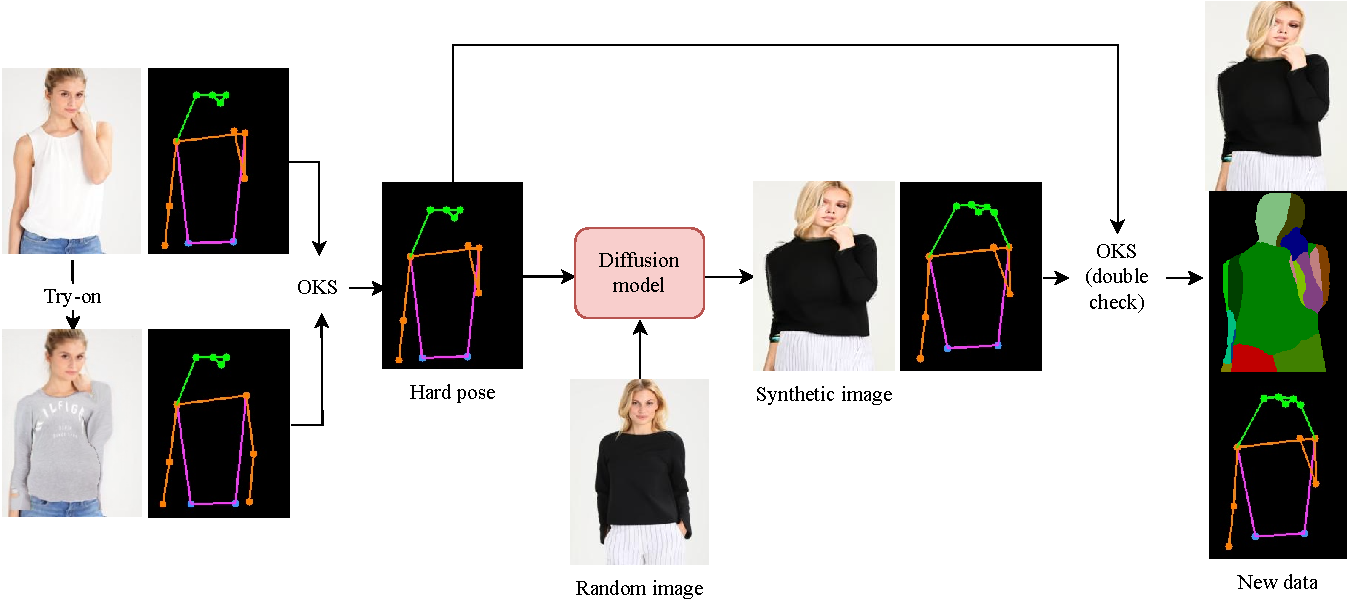
\includegraphics[scale=0.55]{content/resources/images/tryon/augment-pipeline.pdf}
  \caption{Overview of Virtual Try-on-guided Pose for Data Synthesis pipeline.}
   \label{fig:augment-pipeline}
   \vspace{-2mm}
\end{figure}

\begin{figure}[h!]
    \centering
    \subfloat[VITON]{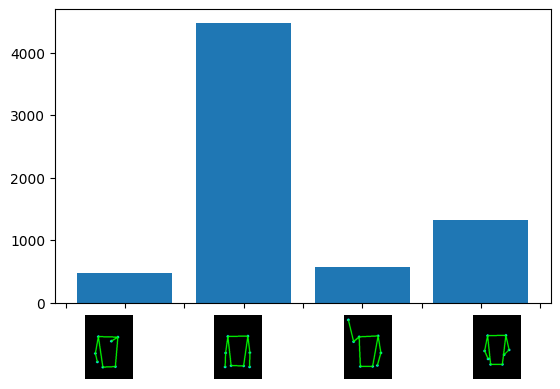
\includegraphics[width=0.45\columnwidth]{content/resources/images/tryon/viton-clean.png}}
    \subfloat[VITON + synthesized data]{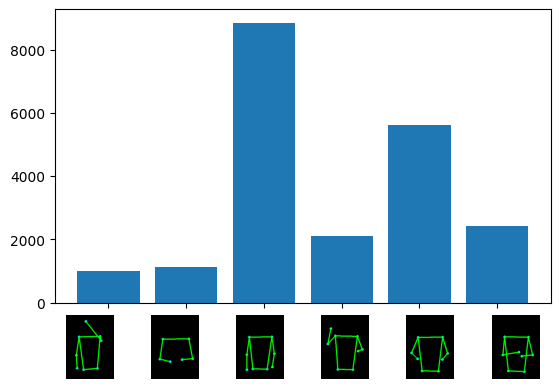
\includegraphics[width=0.45\columnwidth]{content/resources/images/tryon/merge1.png}} 
    \caption{Pose distribution in VITON dataset~\cite{Han-CVPR2018-Viton}.}
    \label{fig:pose-distribution}
    \vspace{-2mm}
\end{figure}

Given an input image containing a person, we extract that person's pose by using the YOLOv7 pose estimation method~\cite{Wang-CVPR2023-YOLOv7}. Then, we utilize our trained DM-VTON model to perform virtual try-on on the input image. The extracted pose from the resulting image is compared with the pose of the input image using a customized OKS metric ~\autoref{formulat:oks}.  

\begin{equation}
    \centering
    \frac{1}{|P|}\sum_{i \in P} \exp(\frac{-d_i^2}{2 s^2 k_i^2}),
    \label{formulat:oks}
\end{equation}
where $P$ denotes the set of arm and hand keypoints, while the original formula uses all keypoints; $d_i$ denotes the Euclidean distance between the keypoint $i$ of two poses; $s$ denotes the total area containing the pose; $k_i$ is the constant provided by Lin et al.~\cite{Lin-ECCV2014-Microsoft} to represent the standard deviation for keypoint $i$. Because we focus on distinguishing different upper-body poses, only the arm and hand keypoints contribute to the formula. If the OKS score falls below a specified threshold $t=0.9$, it is identified as a hard pose.

Once identifying a hard pose, we randomly pick a person image from the VITON dataset. Then it leverages Bhunia's Diffusion model~\cite{Bhunia-CVPR2023-Person} to synthesize a new image of the person in the corresponding pose. To ensure the accuracy of the synthesized image, we perform a double-check using the OKS metric to verify the correctness of the output pose. Finally, DensePose~\cite{Guler-CVPR2018-DensePose} is utilized to generate the body-parser map of the synthesized image.

We initially collected videos from Youtube to synthesize additional data for training networks, specifically focusing on posing or catwalk videos. These videos had varying durations, ranging from 1 to 10 minutes. Subsequently, we extracted individual frames from these videos, which served as the input for our VTP-DS pipeline. %The threshold $t$ for the Object Keypoints Similarity (OKS) metric is set to 0.9. 
After that, we manually removed low-quality results, resulting in 14,314 high-quality synthesized images for training the networks. 

To access the quality of synthesized images, we use the K-means algorithm combined with our modified OKS metric. As details of the pose clustering results shown in~\autoref{fig:pose-distribution}, data in the VITON training set mainly focuses on poses with simple poses (i.e. arms are less covered, low rotation amplitude). Meanwhile, when combined with our synthesized images, new pose clusters appear, and the concentration of data in groups is less imbalanced, which can help to train robust virtual try-on models. 

%%%%%%%%%%%%%%%%%%%%%%%%%%%%%%%%%%%%%%%%%%%%%%%%%%%%%%%%%%%%%%%%
\section{Experiments}
\begin{figure}[h!]
  \centering
  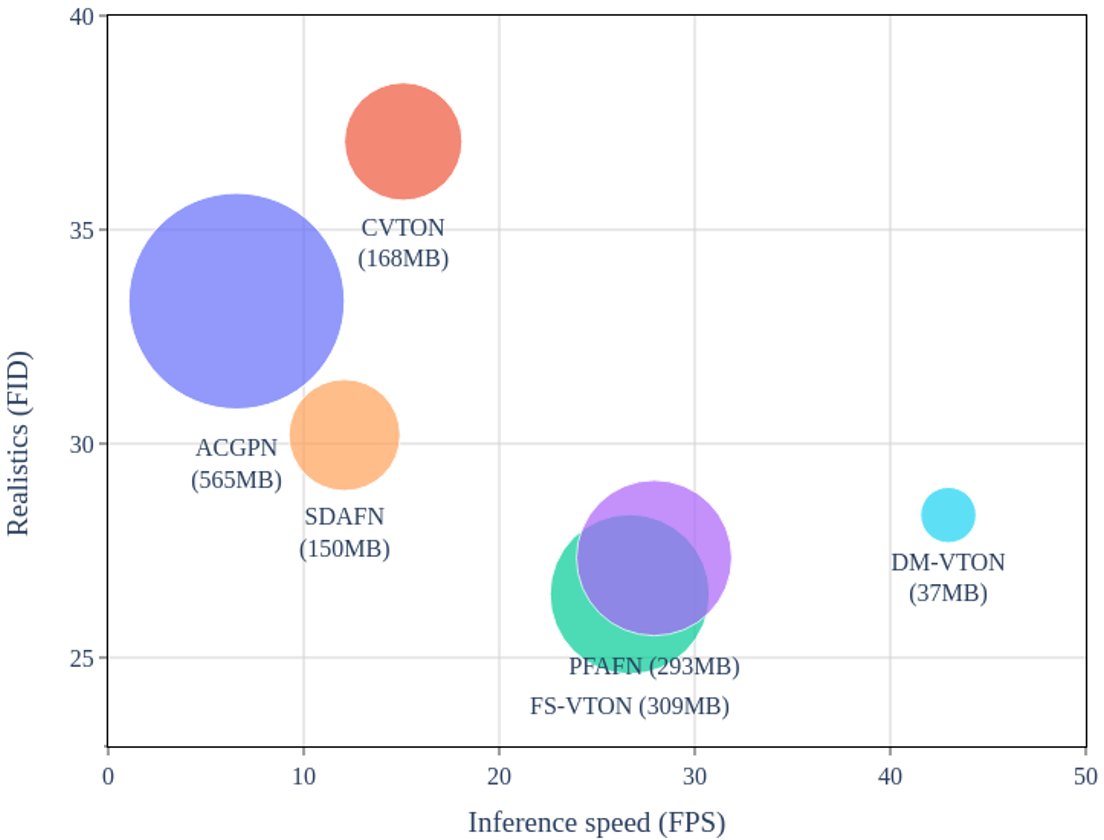
\includegraphics[width=\linewidth]{content/resources/images/tryon/teaser.png}
  \caption{The comparison of our method (DM-VTON) and SOTA methods on VITON test set~\cite{Han-CVPR2018-Viton} in terms of realistic results (FID~\cite{Heusel-NeurIPS2017-FID}, lower is better), inference speed (FPS, higher is better), and memory usage. The size of each bubble represents the memory footprint. FPS is measured using a single Nvidia Tesla T4 GPU.}
  \label{fig:teaser}
  \vspace{-1mm}
\end{figure}

We conducted experiments comparing our DM-VTON framework with other state-of-the-art (SOTA) methods in terms of inference speed, memory usage, and the realisticness of the output. During the experimentation, we carefully evaluated the trade-off between those factors. As depicted in~\autoref{fig:teaser}, our DM-VTON framework outperforms all existing state-of-the-art methods regarding inference speed and memory usage while maintaining an equal quality of results.

\subsection{Detailed Implementation}

% \textbf{Training}: 

The Teacher and Student network training process follows the same strategy with two stages: the first stage only trains the warping module, while the latter trains the entire network. Both were under the same setting and carried out on a single Nvidia A100 GPU. We trained the model for 100 epochs with the initial learning rate is $5 \times 10^{-5}$, which decays linearly after the first 50 epochs.

% \textbf{Testing}: We only use the person and unpaired garment images as input when testing. 

%%%%%%%%%%%%%%%%%%%%%%%%%%%%%%
\subsection{Experimental Settings}
% \subsection{Datasets}

VITON~\cite{Han-CVPR2018-Viton}, the most popular dataset for evaluating virtual try-on, was used to evaluate methods. It contains 16,253 frontal-view upper-body woman and top clothing image pairs with $256 \times 192$ resolution. However, we followed the work of Han et al.~\cite{Han-ICCV2019-Clothflow} to filter out duplicates and ensure no data leakage happens, remaining 6,824 training image pairs and 416 testing image pairs in the cleaned VITON dataset, denoted by VTION-Clean. We combine the VTION-Clean training set and our synthesized images to train our proposed method.

%%%%%%%%%%%%%%%%%%%%%%%%%%%%%% 
% \subsection{Metrics}

Fréchet Inception Distance (FID)~\cite{Heusel-NeurIPS2017-FID} and Learned Perceptual Image Patch Similarities (LPIPS)~\cite{Zhang-CVPR2018-LPIPS} metrics were used to evaluate the similarity of try-on results to real images. 

% \comment{Which methods use their implementation, which methods use their results}

%%%%%%%%%%%%%%%%%%%%%%%%%%%%%% 
\subsection{Experimental Results}
% \subsubsection{Comparision with SOTAs}


% \textbf{Results on VITON dataset}: 
We compared the performance of our proposed MD-VTON with SOTA methods in virtual try-on, such as ACGPN~\cite{Yang-CVPR2020-Towards}, PF-AFN~\cite{Ge-CVPR2021-Parser}, C-VTON~\cite{Fele-WACV2022-CVTON}, SDAFN~\cite{Bai-ECCV2022-Single}, FS-VTON~\cite{He-CVPR2022-Style}. Comparison of MD-VTON against those methods in terms of image quality (i.e., FID and LPIPS), inference speed (i.e., ms), FLOPs (Floating point operations), and memory usage (MB) is shown in~\autoref{table:tryon-speed}. Our proposed method outperforms all other SOTAs in terms of runtime, FLOPs, and memory consumption. On the other hand, our DM-VTON achieves slightly higher FID and LPIPS scores than those of PF-AFN~\cite{Ge-CVPR2021-Parser} and FS-VTON~\cite{He-CVPR2022-Style}. The experimental results prove that the proposed DM-VTON can run in real-time (i.e., 43 frames per second) with small memory consumption but still retains high-quality virtual try-on results. The visualization of compared methods is illustrated in~\autoref{fig:qualitative-viton}.

\begin{table}[h!]
    \centering
    \caption{Quantitative results between DM-VTON and SOTA virtual try-on methods. The $\dagger$ marker indicates the results measured by the generated images provided by the authors. The speed was evaluated on a single Nvidia T4 GPU.}
    %  \comment{what do you mean?}. 
    \label{table:tryon-speed}
    \scriptsize
    \centering
    \resizebox{\textwidth}{!}{
    \begin{tabular}{llcccccccc}
        \toprule
        \textbf{Method}  & \textbf{Published} & Parser & Pose & \textbf{FID $\downarrow$} & \textbf{LPIPS $\downarrow$} & \textbf{Runtime (ms) $\downarrow$} & \textbf{FLOPs (B) $\downarrow$} & \textbf{Memory usage (MB) $\downarrow$}\\
        \midrule
        ACGPN~\cite{Yang-CVPR2020-Towards} & CVPR 2020 & \checkmark & \checkmark & 33.33 & 0.231 & 153.64 & 399.08 & 565.86 \\
        PF-AFN~\cite{Ge-CVPR2021-Parser} & CVPR 2021 & & & 27.33 & 0.216 & 35.80 & 137.85 & 293.25 \\
        C-VTON$\dagger$~\cite{Fele-WACV2022-CVTON} & CVPRW 2022 & \checkmark & & 37.06 & 0.241 & 66.90 & 108.47 & 168.60 \\
        SDAFN~\cite{Bai-ECCV2022-Single} & ECCV 2022 & & \checkmark & 30.20 & 0.245 & 83.42 & 149.40 & 150.87 \\
        FS-VTON~\cite{He-CVPR2022-Style} & CVPR 2022 & & & \textbf{26.48} & \textbf{0.200} & 37.49 & 132.98 & 309.25 \\
        % CP-VTON~\cite{Wang-ECCV2018-Toward} & ECCV 2018 & \checkmark & \checkmark & & & 10.58 & 26.50 & 161.71 \\
        % ClothFlow~\cite{Han-ICCV2019-Clothflow} & ICCV 2019 & \checkmark & \checkmark & & & 20.17 & 16.28 & 44.99 \\
        % WUTON~\cite{Issenhuth-ECCV2020-Do} & ECCV 2020 & & & & & 67.25 & 297.13 & 437.41 \\
        % ShineOn~\cite{Kuppa-WACV2021-ShineOn} & WACV 2021 & \checkmark & & & & 11.43 & 25.95 & 166.85 \\
        % RMGN-VITON~\cite{Lin-IJCAI2022-RMGN} & IJCAI 2022 & & & & & 53.61 & 165.19 & 394.88 \\
        \midrule
        \textbf{DM-VTON} & Ours & & & 28.24 & 0.215 & \textbf{23.27} & \textbf{69.82} & \textbf{37.79} \\
    \bottomrule
    \end{tabular}}
\end{table}


% \begin{table}[h!]
%     \centering
%     \caption{Quantitative results between DM-VTON and SOTA virtual try-on methods. The $\dagger$ marker indicates the results measured by the generated images provided by the authors. The speed was evaluated on a single Nvidia T4 GPU.}
%     %  \comment{what do you mean?}. 
%     \label{table:tryon-speed}
%     \scriptsize
%     \centering
%     \resizebox{\textwidth}{!}{
%     \begin{tabular}{lccccccc}
%         \toprule
%         \textbf{Method} & Parser & Pose & \textbf{FID $\downarrow$} & \textbf{LPIPS $\downarrow$} & \textbf{Runtime (ms) $\downarrow$} &  \textbf{Memory usage (MB) $\downarrow$}\\
%         \midrule
%         ACGPN (Yang et al., 2020) & \checkmark & \checkmark & 33.33 & 0.231 & 153.64 & 565.86 \\
%         PF-AFN (Ge et al., 2021) & & & 27.33 & 0.216 & 35.80 & 293.25 \\
%         C-VTON$\dagger$ (Fele et al., 2022) & \checkmark & & 37.06 & 0.241 & 66.90 & 168.60 \\
%         SDAFN (Bai et al., 2022) & & \checkmark & 30.20 & 0.245 & 83.42 & 150.87 \\
%         FS-VTON (He et al., 2022) & & & \textbf{26.48} & \textbf{0.200} & 37.49 & 309.25 \\
%         % CP-VTON~\cite{Wang-ECCV2018-Toward} & ECCV 2018 & \checkmark & \checkmark & & & 10.58 & 26.50 & 161.71 \\
%         % ClothFlow~\cite{Han-ICCV2019-Clothflow} & ICCV 2019 & \checkmark & \checkmark & & & 20.17 & 16.28 & 44.99 \\
%         % WUTON~\cite{Issenhuth-ECCV2020-Do} & ECCV 2020 & & & & & 67.25 & 297.13 & 437.41 \\
%         % ShineOn~\cite{Kuppa-WACV2021-ShineOn} & WACV 2021 & \checkmark & & & & 11.43 & 25.95 & 166.85 \\
%         % RMGN-VITON~\cite{Lin-IJCAI2022-RMGN} & IJCAI 2022 & & & & & 53.61 & 165.19 & 394.88 \\
%         \midrule
%         \textbf{DM-VTON} (Ours) & & & 28.24 & 0.215 & \textbf{23.27} & \textbf{37.79} \\
%     \bottomrule
%     \end{tabular}}
% \end{table}


\begin{figure}[h!]
  \centering
  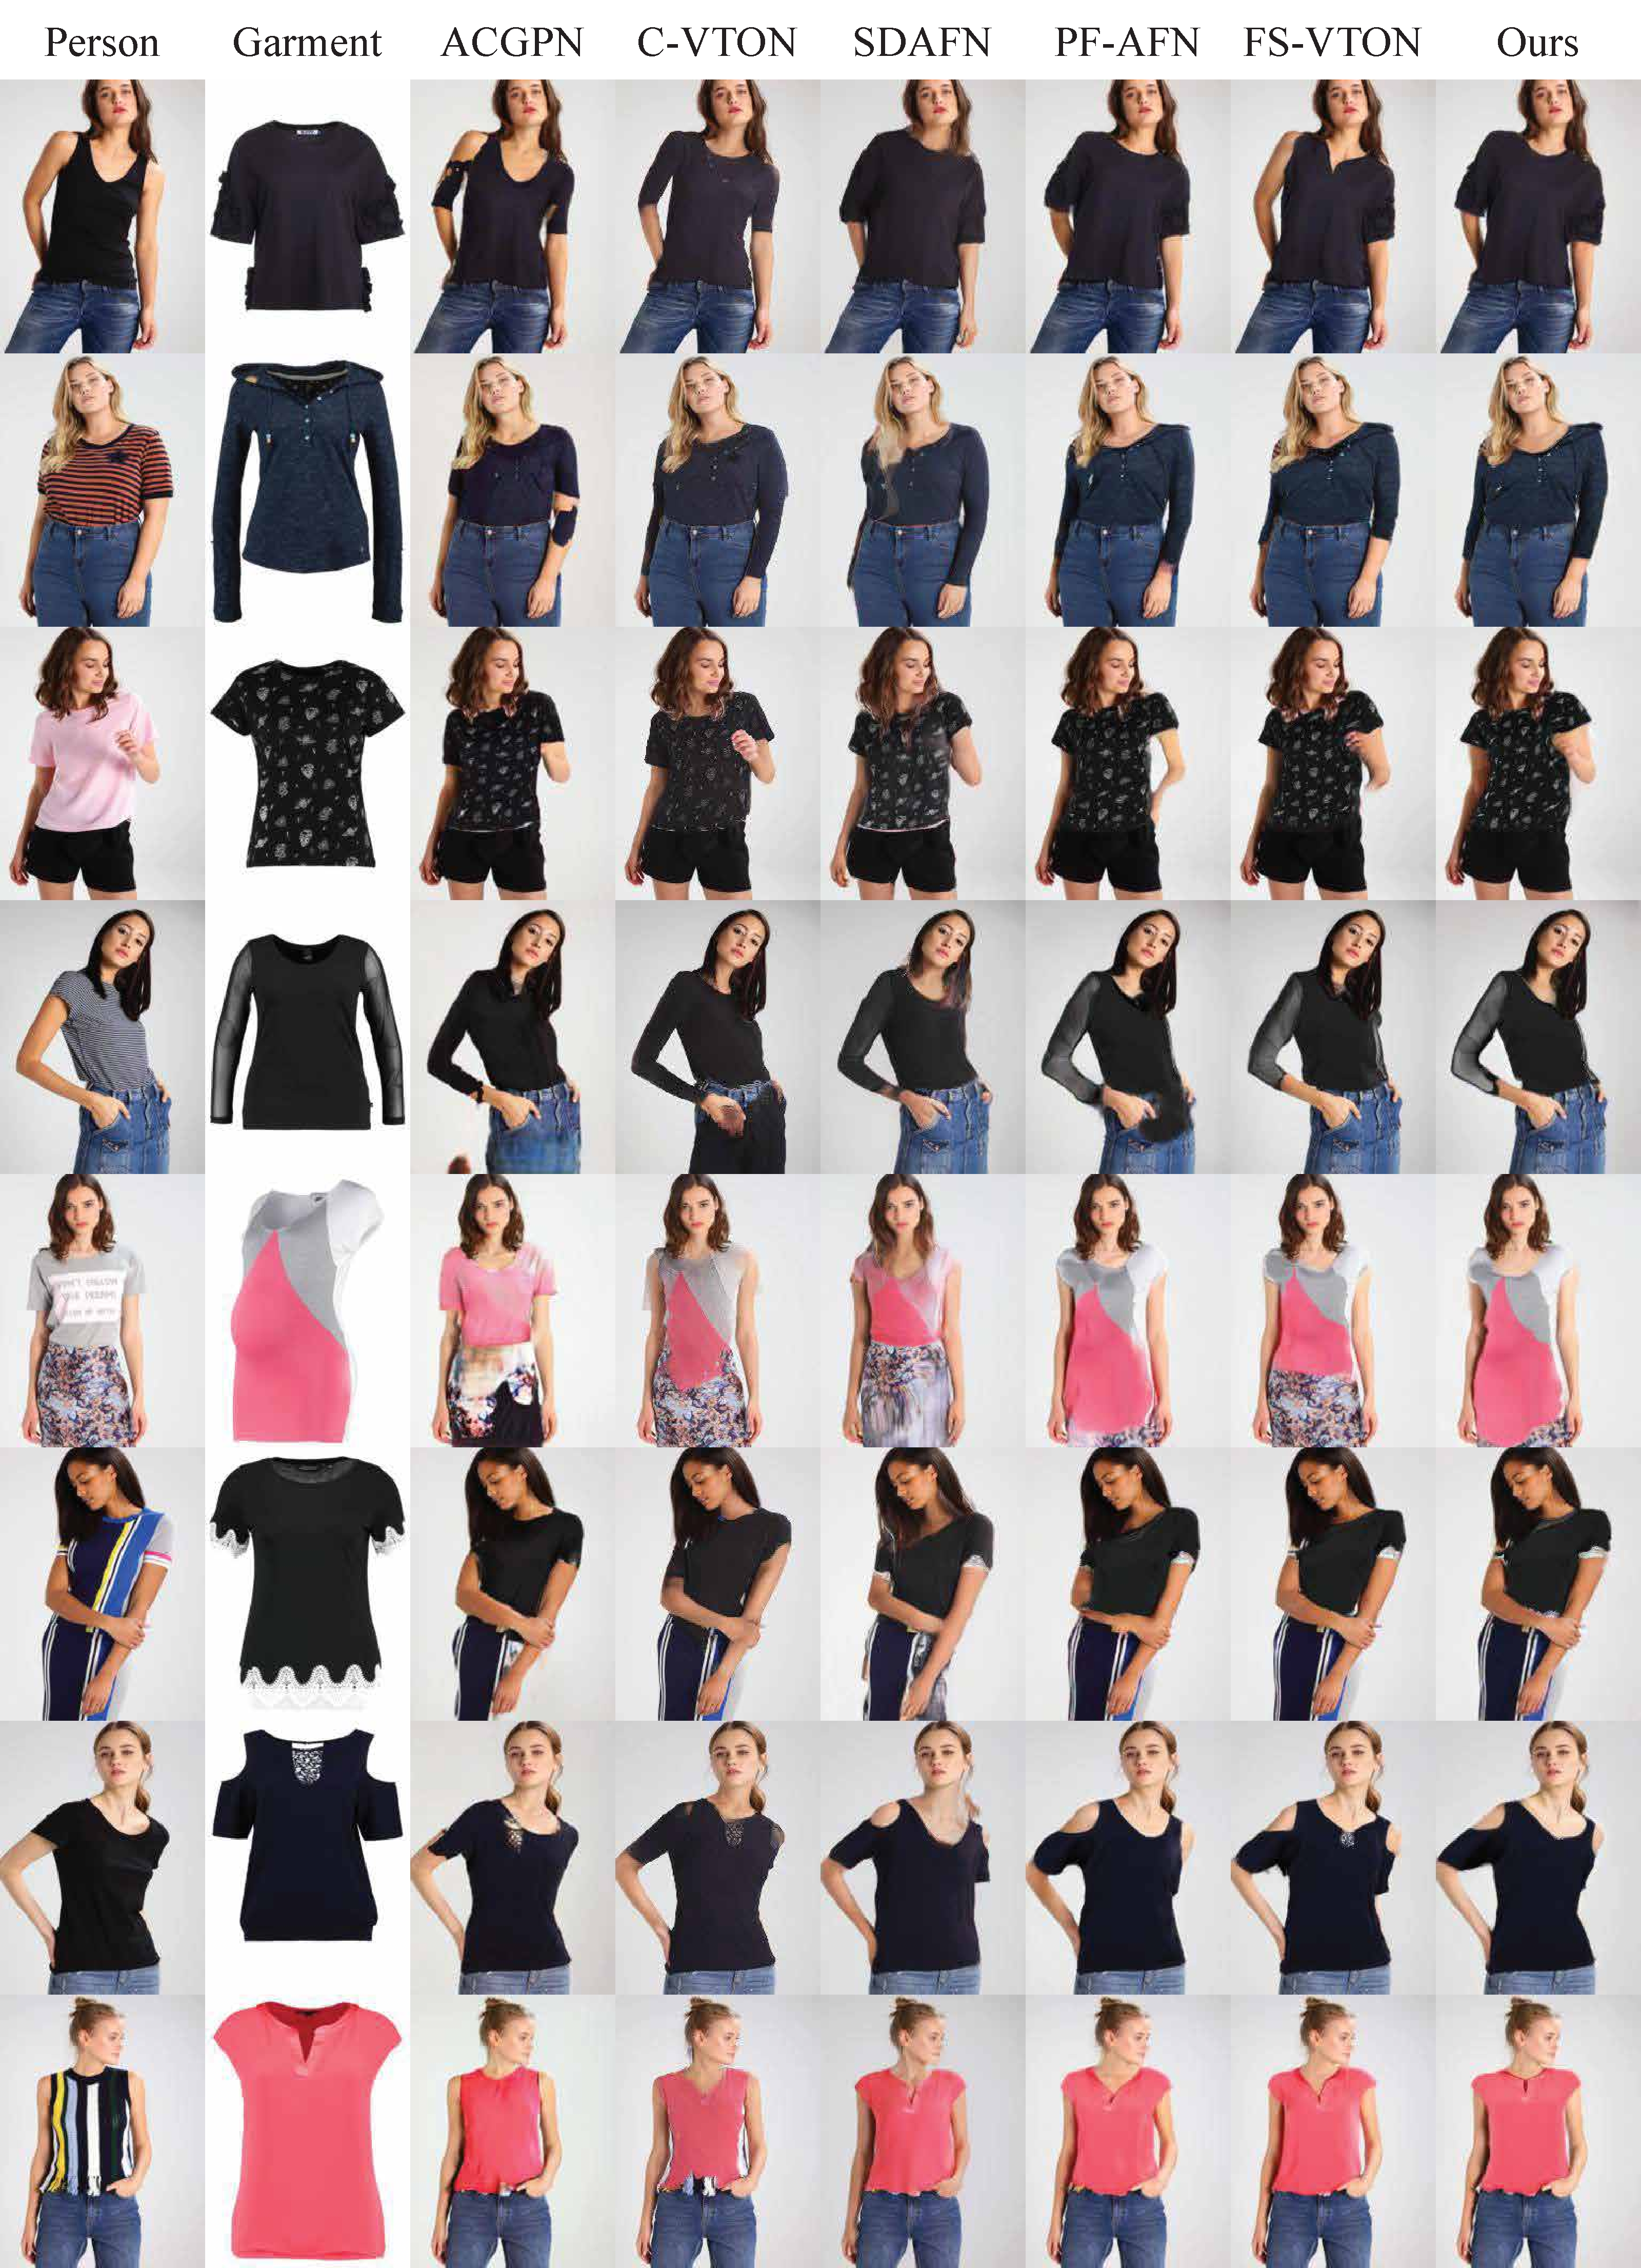
\includegraphics[width=\linewidth]{content/resources/images/tryon/qualitative-viton.pdf}
  \caption{Qualitative comparison on VITON-Clean dataset~\cite{Han-CVPR2018-Viton}.}
  \label{fig:qualitative-viton}
  \vspace{-2mm}
\end{figure}

%%%%%%%%%%%%%%%%%%%%%%%%%%%%%%%%%%%%%%%%%%%%%%%%%%%%%%%%%%%%%%%%
% \section{Fashion Recommendation}
% \subsection{Done}
% \subsubsection{Dataset}
% We conduct our experiments on the PolyvoreOutfits dataset \cite{Mariya-ECCV18-Learning}. The dataset has 251.008 fashion items, with 11 main categories (glasses, shoes, accessories, jewelry, scarves, bottoms, hats, outerwear, tops, bags, and all-body). These main categories are further divided into 153 subcategories with no semantic meaning. The dataset also has 2 subsets: disjoint set and non-disjoint set. The disjoint set has 35.140 outfits, and the non-disjoint set has 68.306 outfits. An item can appear in multiple outfits. The disjoint set has a stricter rule about the appearance of an item, each item can only be seen in one of the train/validation/test sets. Meanwhile, in the non-disjoint set, an item can appear in all train/validation/test sets. To limit the scope, we only use the disjoint set. \autoref{fig:disjoint-categories} shows the number of items in each category in the disjoint set.

% \begin{figure}[h!]
%   \centering
%   \includegraphics[width=0.7\linewidth]{Recommendation/disjoint_category.png}
%   \caption{Histogram of categories in the disjoint set}
%   \label{fig:disjoint-categories}
% \end{figure}

% \subsubsection{Fine-tuning metrics}
% To evaluate the recommendation quality between our finetuned models, we use the metric recall at K with the following setups, for each masked item:
% \begin{enumerate}
%     \item Find K items within the same category as the masked item.
%     \item If those K items contain the masked item, count as correct.
% \end{enumerate}
% The final result is the number of correct items / number of masked items * 100.

% \subsubsection{Loss function} We compare 2 losses: Mean Squared Error (\autoref{fig:mse-loss} and Contrastive loss (\autoref{fig:contrastive-loss}). We train the model by randomly masking 1 item in each outfit of the training set, and we validate the model by randomly masking 1 item in each outfit of the validation set. We find that MSE loss is faster to converge but the recall is relatively low, even at higher recall rank. Meanwhile, the contrastive loss still can converge more and also achieve higher recall.

% \begin{figure}[h!]
%   \centering
%   \includegraphics[width=0.7\linewidth]{Recommendation/MSE loss, mask 1.png}
%   \caption{MSE loss, train set (top), validation set (bottom)}
%   \label{fig:mse-loss}
% \end{figure}

% \begin{figure}[h!]
%   \centering
%   \includegraphics[width=0.7\linewidth]{Recommendation/Contrastive, mask 1.png}
%   \caption{Constrastive loss, train set (top), validation set (bottom)}
%   \label{fig:contrastive-loss}
% \end{figure}

% \subsubsection{Normalization the output} Before searching the query vector in the dataset, we have to normalize it. With the same mask setup as above, when conducting some experiments, we discover that normalizing the vector before calculating the loss harms the model. 
% \autoref{fig:contrastive-loss} shows the result of normalizing before feeding to the loss, \autoref{fig:contrastive-loss-no-norm} is the results of normalization after that. When removing the last normalization during the training process, we can get higher recall and also some signs of overfitting.

% \begin{figure}[h!]
%   \centering
%   \includegraphics[width=0.7\linewidth]{Recommendation/Contrastive, mask 1, no norm.png}
%   \caption{Constrastive loss w/o normalization, train set (top), validation set (bottom)}
%   \label{fig:contrastive-loss-no-norm}
% \end{figure}

% \subsubsection{Mask percentage} As our problem is to predict multiple categories at once, we try increasing the mask percentage. We train our model while masking 50\% of items in each outfit of the training dataset and perform the validation by masking 1 item in each outfit of the validation dataset. The result is shown in \autoref{fig:contrastive-loss-no-norm-mask-half}. The validation recall is still the same as when we only mask 1 item, which means the model can learn even with fewer input items. We further evaluate the best validation model on the test dataset with different mask ratios and recall ranks, as shown in \autoref{fig:test-mask-ratio}. The recall drops significantly when we mask 70\% of the items while slowly drops when masking fewer items.


% \begin{figure}[h!]
%   \centering
%   \includegraphics[width=0.7\linewidth]{Recommendation/Contrastive, mask half, no norm.png}
%   \caption{Constrastive loss w/o normalization, mask 50\%, train set (top), validation set (bottom)}
%   \label{fig:contrastive-loss-no-norm-mask-half}
% \end{figure}

% \begin{figure}[h!]
%   \centering
%   \includegraphics[scale=0.4]{Recommendation/Masked ratio.png}
%   \caption{Test set recall by masked ratio}
%   \label{fig:test-mask-ratio}
% \end{figure}

% \subsubsection{SOTA metric}
% Current State-of-the-art papers \cite{Yen-CVPR2020-Fashion, Han-ECCV2022-FashionViL, Sarkar-CVPRW2022-OutfitTransformer} use a subset of the PolyvoreOutfits test set for evaluation, proposed by \cite{Yen-CVPR2020-Fashion}. They calculate the recall at rank K on the fill-in-the-blank problem:
% \begin{enumerate}
%     \item For each outfit, choose 1 item to mask. (the mask item id is predefined, not randomly)
%     \item Find K items within the same subcategory as the masked item.
%     \item If those K items contain the masked item, count as correct.
% \end{enumerate}
% The final result is the number of correct items / number of masked items * 100. The comparison between our model and other SOTA methods is shown in \autoref{table:outfit-SOTA-compare}. This shows that our model cannot achieve as high results as their methods in the single-item fill-in-the-blank problem. 

% \begin{table}[h!]
% \centering
% \begin{tabular}{l c c c}
% \hline
%                                  & K = 10        & K = 30         & K = 50         \\ \hline
% Type-Aware \cite{Mariya-ECCV18-Learning}           & 3.66          & 8.26           & 11.98          \\
% CSA-Net \cite{Lin2020}              & 5.93          & 12.31          & \textbf{17.85} \\
% FashionVIL \cite{Han-ECCV2022-FashionViL}           & 5.83          & \textbf{12.61} & 17.49          \\
% OutfitTransformer   \cite{Sarkar-CVPRW2022-OutfitTransformer} & \textbf{6.53} & 12.12          & 16.64          \\ 
% Ours                             & 4.19          & 8.55           & 11.96          \\ \hline
% \end{tabular}
% \caption{Recall between our methods and other SOTA}
% \label{table:outfit-SOTA-compare}
% \end{table}

% The histogram of the false negative results is shown in \autoref{fig:neg-sample-category}. It looks like the \autoref{fig:disjoint-categories} a lot, especially the "shoes" and "bags" categories. The higher the number of items in a category, the easier to recommend false negative items. \autoref{fig:neg-sample} shows some false negative samples. From our perspective, the recommendation results are still acceptable. Everyone has different tastes in fashion, so the ground truth items may not be the most compatible items for everyone.

% \begin{figure}[h!]
%   \centering
%   \includegraphics[scale=0.2]{Recommendation/neg_sample_by_categories.png}
%   \caption{False negative histogram by categories}
%   \label{fig:neg-sample-category}
% \end{figure}

% \begin{figure}[h!]
%   \centering
%   \includegraphics[width=0.8\linewidth]{Recommendation/neg-samples.png}
%   \caption{False negative samples, the true positive items are colored red, each following line is the recommendation result}
%   \label{fig:neg-sample}
% \end{figure}

% \subsection{Doing}
% \subsubsection{Replace KNN with ANN} We prepare a dataset include 774400 images (from \cite{Mariya-ECCV18-Learning, Liu-CVPR2016-DeepFashion}, extract their embeddings using \cite{Baldrati-CVPR2022-Effective} pretrained CLIP models. We conduct our experiments with the following settings:
% \begin{enumerate}
%     \item Search space: 30K items, 70K items, 300K items, full dataset (774k items)
%     \item Query item: randomly select one item in the search space.
%     \item Algorithms: KNN\footnote{\label{faiss}https://github.com/facebookresearch/faiss}, LSH\footref{faiss}, IVF\footref{faiss}, IVF+PQ\footref{faiss}, HNSW\footref{faiss}, ANNOY\footnote{https://github.com/spotify/annoy}
%     \item Metrics: Search time, memory usage, recall at rank 100 (KNN results as the ground truth)  
% \end{enumerate}

% \blue{Note}:
% LSH: get saturaion point value
% IVF + Annoy: get until 0.98 recall
% IVFPQ: Use IVF params with maximize number of sub vectors
% HSNW: min to get 0.98 recall

% \subsection{To do}
% \subsubsection{Human studying}
% As our problem, recommending multiple categories at the same time, is novel. There have been no metrics or datasets to evaluate the search quality. Also, everyone has different tastes in their fashion style. We plan to perform human studying on 15 people (more is better) whether they find the complementary items compatible with the query item. The metric is calculated as (the number of compatible items / the number of items asked).
\chapter{Fashion Recommendation}
\label{chapter-fashion-recommendation}
\begin{ChapAbstract}
In this chapter, we address the problem of recommending items given a reference fashion item. We carefully investigate three approaches to retrieving items: similar items within the same category, complementary items from other categories, and items guided by text feedback. 
In terms of retrieving intra-category similar items and text feedback-guided items, we employ a pretrained CLIP-based model and receive remarkable results. As for the inter-category complementary item retrieval, we consider it a Natural Language Process problem and propose Outfit Retrieval Transformers (ORT), which utilizes the Transformers architecture. Through experiments, ORT proves its effectiveness and can produce reasonable recommendations. Because using an embedding to query items from a dataset plays an important role in recommendation, we analyze various approximate searching methods and compare them with the exhaustive K-Nearest Neighbor algorithm regarding query time and accuracy.
\end{ChapAbstract}

\section{Overview}
Fashion recommendation involves retrieving items from a fashion dataset based on some given information and proposing them to users. To limit the scope, in this thesis, we take an input garment as the reference item and investigate three approaches to retrieving items based on the visual feature of that item. 

\begin{figure}[t!]
    \centering
    \includegraphics[width=\linewidth]{content/resources/images/fashion-recommendation/chapter4-overview.pdf}
    \caption{Our investigation scope on fashion recommendation}
    \label{fig:chapter4-overview}
\end{figure}

The first approach is \textbf{intra-category similar item retrieval}, where we search for items within the same category and with similar visual representations to the reference item. 

The second approach, called \textbf{inter-category complementary item retrieval}, broadens the scope by considering items from different categories that complement the reference item to make a complete outfit. We define a complete outfit as an outfit that contains at most one item of each category, and all items share a similar style or are visually compatible. This approach differs from the fill-in-the-blank task described in PolyvoreOutfits~\cite{Mariya-ECCV18-Learning}, where each outfit has only one missing item. Our problem is more generalized, allowing for varying numbers of missing items in an outfit.
The last approach we investigate in this thesis is \textbf{text feedback-guided item retrieval}. In this approach, we aim to find fashion items that satisfy the constraints expressed in the user's feedback, provided in natural language. The feedback may describe relative attributes such as being more formal or having longer sleeves.  

In all mentioned approaches, after extracting the visual features of the desired items, we utilize the PolyvoreOutfits dataset~\cite{Mariya-ECCV18-Learning} and search through the embedded features of all items to find the most similar ones. This dataset contains metadata for 251,008 fashion items, and 35,140 outfits, and covers 11 categories: bags, tops, outerwear, hats, bottoms, scarves, jewelry, accessories, shoes, and sunglasses. Due to the dataset's scale, we explore the use of approximate search methods \cite{Sivic-ICCV2003-Video, Erik-Github-Annoy, Malkov-TPAMI2018-Efficient} instead of the commonly used exhaustive K-Nearest Neighbor method for more efficient searching. \autoref{fig:chapter4-overview} illustrates our investigation scope on fashion recommendation.

\begin{figure}[b]
    \centering
    \includegraphics{content/resources/images/fashion-recommendation/chapter4-clip.pdf}
    \caption{CLIP learning process}
    \label{fig:chapter4-clip}
\end{figure}

\section{Dataset Preprocessing}
As we use the visual features of items in the dataset in every search, we extract the visual embedding of all items beforehand and use them directly in later searches. In this thesis, we utilize CLIP~\cite{Radford-OpenAIblog2019-Language}, which learns joint representations of images and their corresponding textual descriptions (\autoref{fig:chapter4-clip}), to encode all items. Both the Image and Text Encoder of CLIP are built upon the Transformer Encoder~\cite{Vaswani-NeurIPS2017-Attention} block. By passing an image through the CLIP model, we obtain a visual embedding that captures its visual features and semantic information.


\section{Intra-category Similar Item Retrieval}
In terms of intra-category similar item retrieval, we first extract the visual embeddings of the reference image using the same CLIP model that we used to extract the embeddings of all items in our dataset. Subsequently, the approximate searching algorithm uses the extracted features to retrieve similar items from the PolyvoreOutfits dataset. \autoref{fig:chapter4-similar} illustrates our similar item retrieval pipeline.

\begin{figure}[h!]
    \centering
    \includegraphics[width=\linewidth]{content/resources/images/fashion-recommendation/chapter4-similar.pdf}
    \caption{Similar item retrieval pipeline}
    \label{fig:chapter4-similar}
\end{figure}

\section{Inter-category Complementary Item Retrieval}
We address the inter-category complementary item retrieval task as the sentence generation task in the natural language domain. Transformers~\cite{Vaswani-NeurIPS2017-Attention}, a deep learning architecture for natural language processing (NLP) tasks, has proven its efficiency in generating a complete sentence from some given keywords~\cite{bhatia-github-keytotext} or a partial sentence~\cite{Devlin-ArXiv2018-BERT}.

In this thesis, we investigate using the Transformers architecture to retrieve complementary items and make a complete outfit. We name this method \textbf{O}utfit \textbf{R}etrieval \textbf{T}ransformers (ORT). Specifically, we consider a complete outfit as a sequence of fashion items, where the order is determined by their categories: bags, tops, outerwear, hats, bottoms, scarves, jewelry, accessories, shoes, and sunglasses. Not all categories are required. All items in an outfit are divided into three groups: \textit{Input}, \textit{Output}, and \textit{Unavailable}. The division of items among these groups depends on whether it's the training or inference phase.

PolyvoreOutfits~\cite{Mariya-ECCV18-Learning} dataset provides us with the metadata of over 35,000 complete outfits, including which items belong to each outfit. Thus, in the training phase, we divide items into an outfit as follows:
\begin{itemize}
    \item \textit{Input} items are selected randomly from the available items.
    \item The remaining items within available items are \textit{Outfit} items.
    \item Items in categories that the outfit lacks are denoted as \textit{Unavailable}.
\end{itemize}

During the inference phase, as we generate complementary items for the reference item, we use the following division:
\begin{itemize}
    \item \textit{Input} item is the reference item only.
    \item \textit{Output} items belong to categories that we aim to propose to users. These items are our target complementary items.
    \item Items in the remaining categories are denoted as \textit{Unavailable}.
\end{itemize}

Each group of items has different ways to represent their embedding:
\begin{itemize}
    \item \textit{Input}: the item's visual embedding as-is.
    \item \textit{Output}: a shared, learnable embedding, denoted as \textit{<OUT>}.
    \item \textit{Unavailable}: a shared, learnable embedding, denoted as \textit{<UN>}.
\end{itemize}

\begin{figure}[h!]
    \centering
    \subfloat[Train phase]{\includegraphics[width=\linewidth]{content/resources/images/fashion-recommendation/chapter4-comp-train.pdf}}
    \hspace{0.5cm}
    \subfloat[Inference phase]{\includegraphics[width=\linewidth]{content/resources/images/fashion-recommendation/chapter4-comp-test.pdf}} 
    \caption{Outfit Retrieval Transformers pipeline.}
    \label{fig:chapter4-outfit-trans}
\end{figure}

All embeddings are fed into a Transformers Encoder block~\cite{Vaswani-NeurIPS2017-Attention} to produce cross-semantic-aware output embeddings (as shown in \autoref{fig:chapter4-outfit-trans}). ORT also use positional embeddings technique~\cite{Vaswani-NeurIPS2017-Attention}, where each position specifies the item's category. During the training phase, the network minimizes the noise contrastive loss~\cite{Lai-Arxiv2019-Contrastive} so the Transformers block learns to maximize the similarity between its output embeddings and the \textit{Output} items' original visual embeddings (as shown in \autoref{fig:chapter4-outfit-trans}(a)). We formulate the loss $L$ as follows:
\begin{align}
    & L = -\frac{1}{N}*\Sigma_{i=1}^{N} log{\frac{exp(S_{i_P})}{exp(S_{i_P}) + exp(S_{i_N})}},\\
    & S_{i_P} = cos(pred_i, pos_i),\\
    & S_{i_N} = \Sigma_{j \in {neg_i}} cos(pred_i, j),
\end{align}

where $N$ is the number of \textit{Output} items in all outfits, $pred_i$ is the $i^{th}$ predicted output embeddings, $pos_i$ is the ground-truth visual embeddings of that \textit{Output} item, $neg_i$ is a set of negative samples which contains the embeddings of other items of the same category. 

During the inference phase, we utilize the approximate searching algorithm to retrieve similar items from ORT's output embeddings (as shown in \autoref{fig:chapter4-outfit-trans}(b)).

\section{Text Feedback-guided Item Retrieval}
To address this task, we adopt the CLIP4Cir architecture proposed by Baldrati et al~\cite{Baldrati-CVPR2022-Conditioned}. The architecture proves efficiency despite its simplicity. It first utilizes CLIP model~\cite{Radford-OpenAIblog2019-Language} to extract embeddings from both the reference image and relative feedback. Then, both embeddings are fed into a Combiner network, a small trainable network specifically designed to merge the two embeddings into a single output embedding (as shown in \autoref{fig:chapter4-combiner}).

\begin{figure}[t!]
    \centering
    \includegraphics[width=\linewidth]{content/resources/images/fashion-recommendation/chapter4-combiner.pdf}
    \caption{Combiner architecture}
    \label{fig:chapter4-combiner}
\end{figure}


\begin{figure}[t!]
    \centering
    \subfloat[Train phase]{\includegraphics[width=0.85\columnwidth]{content/resources/images/fashion-recommendation/chapter4-clip4cir-train.pdf}}
    \hspace{0.5cm}
    \subfloat[Inference phase]{\includegraphics[width=\columnwidth]{content/resources/images/fashion-recommendation/chapter4-clip4cir-test.pdf}} 
    \caption{CLIP4Cir pipeline.}
    \label{fig:chapter4-clip4cir}
\end{figure}

During the training phase, we utilize the FashionIQ dataset~\cite{Wu-CVPR2021-FashionIQ}, which consists of triplet pairs comprising a reference image, relative feedback, and a target image. The Combiner is trained to maximize the similarity between its output embeddings and the target images' embeddings produced by CLIP (\autoref{fig:chapter4-clip4cir}(a)), specified by the following symmetric contrastive loss $L$:
\begin{align}
    & L = \frac{1}{2}(L_c + L_i),\\
    & L_c = \text{cross\_entropy\_loss}(E_cE_i, logits),\\
    & L_i = \text{cross\_entropy\_loss}(E_iE_c, logits),
\end{align}

where $logits$ denotes the list $\{1, 2, ..., N\}$ with $N$ is the batch size, $E_c$ denotes a batch of Combiner's output embeddings and $E_i$ denotes a batch of CLIP's output embeddings. This shared representation space allows us to effectively compare the similarity between the embeddings produced by the Combiner and CLIP.

To run inference, we also leverage the approximate searching algorithm to retrieve similar items for the target output embeddings (as shown in \autoref{fig:chapter4-clip4cir}(b)).

\section{Approximate Searching}
In all of the three recommendation approaches we have investigated so far, the final involves retrieving the items from the dataset that have visual embeddings most similar to a given input embedding.

For such nearest neighbor problem, K-Nearest Neighbor (KNN) algorithm are widely used due to its simplicity and giving exact results(\cite{Lin-CVPR2020-Fashion, Baldrati-CVPR2022-Conditioned, Baldrati-CVPR2022-Effective, Sarkar-CVPRW2022-OutfitTransformer}.  The KNN algorithm exhaustively searches through every dimension of all items in the dataset. As a result, this algorithm has the runtime complexity of $O(kNd)$ where $k$ is the number of items to retrieve, $N$ is the size of the dataset, and $d$ is the number of dimensions to represent one item, in our case, it is the length of the visual embedding produced by CLIP~\cite{Radford-OpenAIblog2019-Language}. 

Approximate searching algorithms solve this problem by lowering either $N$ or $d$, thus allowing the search faster with the accuracy trade-off. Approximate methods also help compress the dataset due to the decline of $d$~\cite{Gionis-VLDB1999-Similarity, Jegou-TPAMI2010-Product}. However, as mentioned in Jegou's work~\cite{Jegou-ICASSP2011-IVFPQ}, these methods significantly decrease the result accuracy.  In this thesis, our primary goal is to find the fastest approximate methods while keeping a reasonable accuracy. Thus, we focus on investigating three common algorithms that lower the search space $N$: Inverted File Index~\cite{Sivic-ICCV2003-Video} (IVF), Hierarchical Navigable Small Worlds~\cite{Malkov-TPAMI2018-Efficient} (HNSW), and Approximate Nearest Neighbors Oh Yeah~\cite{Erik-Github-Annoy} (ANNOY). We use the Euclidean metric as our distance metric while retrieving nearest neighbors.

\subsection{Inverted File Index (IVF)}
The basic idea behind the Inverted File Index~\cite{Sivic-ICCV2003-Video} is to partition the dataset into multiple subsets, usually done by employing K-Means. We denote the number of subsets as $nlist$. Subsequently, all embeddings in the dataset are stored separately in their corresponding subset. Each subset also contains a centroid, which is the mean of all embeddings in that subset. 

We calculate the distance between the input embedding and all centroids during the query process and take the closest one. Then, we only search through all items in the corresponding subset. This means the larger $nlist$, the smaller subset we need to search through. 

\begin{figure}[h!]
    \centering
    \includegraphics[width=0.7\linewidth]{content/resources/images/fashion-recommendation/chapter4-ivf.png}
    \caption{The case where the query embedding falls on the outskirts of the closest subset in IVF}
    \label{fig:chapter4-ivf}
\end{figure}

However, if the query embedding falls on the outskirts of the closest subset, its nearest neighbors may belong to nearby clusters (\autoref{fig:chapter4-ivf}). This is what makes this method approximate and not exact. The impact can be reduced by searching for multiple nearby subsets; we denote the number of subsets to search as $nprobe$. A larger $nprobe$ means taking more time but giving better accuracy. The number of subsets $nlist$ and the number of subsets to search $nprobe$ can be tuned to find the time/accuracy reasonable trade-off. 

\subsection{Approximate Nearest Neighbors Oh Yeah (ANNOY)}
ANNOY~\cite{Erik-Github-Annoy} is the search algorithm used by Spotify in their music recommendation system~\cite{Erik-Github-Annoy}. The key idea of ANNOY is to build a binary tree, where each leaf node is an item in the dataset. ANNOY selects a random hyperplane to partition the dataset into two subsets at each intermediate node in the tree construction process. This hyperplane is determined by sampling two random points from the corresponding subset and taking the hyperplane equidistant from them. The construction process is shown in \autoref{fig:chapter4-annoy}. The constructed tree structure is stored alongside the dataset.

\begin{figure}[thb!]
    \centering
    \subfloat[Construction process]{\includegraphics[width=0.9\columnwidth]{content/resources/images/fashion-recommendation/chapter4-annoy-step.png}}
    \hspace{0.1mm}
    \subfloat[Constructed tree]{\includegraphics[width=0.5\columnwidth]{content/resources/images/fashion-recommendation/chapter4-annoy-tree.png}} 
    \caption{ANNOY index construction process}
    \label{fig:chapter4-annoy}
\end{figure}

We traverse the binary tree from the root during the query process by repeatedly checking which side of the corresponding hyperplane the query embedding belongs to.
This method also faces the same issue as IVF; if the query item falls on the outskirts of a subspace, the nearest neighbors may appear in sibling leaf nodes instead. To tackle this problem, ANNOY allows searching for multiple leaf nodes, which can be done by using a priority queue to keep track of the closest hyperplane so we can backtrack to that hyperplane and go to the other side. ANNOY also proposes building multiple trees at once to minimize the effect of randomness. 

We denote the number of trees to build as $n\_{trees}$ and the total number of leaf nodes to search in all trees as $search\_k$. A larger $n\_{trees}$ gives more accurate results but larger memory usage; it does not affect the query time. A larger $search\_k$ leads to more accurate results but longer query time.

\subsection{Hierarchical Navigable Small Worlds (HNSW)}
The key idea of Hierarchical Navigable Small Worlds~\cite{Malkov-TPAMI2018-Efficient} (HNSW) is taken from the Skip List data structure. Skip List is a data structure that consists of multiple sorted linked lists. The bottom level (or level 0) is the ordinary linked list containing all the elements. The higher levels contain fewer elements and act as shortcuts to traverse the list quickly. \autoref{fig:chapter4-skiplist} illustrates the Skip List data structure.

\begin{figure}[th!]
    \centering
    \includegraphics[width=\linewidth]{content/resources/images/fashion-recommendation/chapter4-skiplist.pdf}
    \caption{Skip list data structure}
    \label{fig:chapter4-skiplist}
\end{figure}

To search in a Skip List, we start at the highest level, which has the longest step between elements and iterate towards the end of that level. If the current element is greater than the search value, we move down to the previous node in the \textit{below} level. This process repeats until we find the search value or reach the lowest level (level 0) (as shown in \autoref{fig:chapter4-skiplist-search}).

\begin{figure}[th!]
    \centering
    \includegraphics[width=\linewidth]{content/resources/images/fashion-recommendation/chapter4-skiplist-search.pdf}
    \caption{Skip list search process}
    \label{fig:chapter4-skiplist-search}
\end{figure}

HNSW borrows that idea and applies it in higher dimensions. Specifically, HNSW constructs multiple undirected graphs, where the graph at the lowest level (level 0) contains all dataset items as its nodes. The higher-level graphs contain fewer nodes, leading to longer distances between each node. To reduce the number of adjacent nodes during traversing, HNSW limits the maximum degree of each node in all graph levels, denoted as $M$. The HNSW data structure is constructed from a dataset by inserting each embedding vector one by one. Given $M$ is the maximum degree of each node, $efConstruction$ and $efSearch$ are the maximum numbers of nodes to traverse at each level in the index and query process, respectively, the steps to insert a new embedding vector are as follows:
\begin{enumerate}
    \item If this is the first item, insert it to all levels and continue.
    \item Find the graph level $L$ to insert the new item. The value of $L$ has exponentially decreasing probability as it goes higher, specified by the equation $L = max(floor(-log(uniform(0, 1))), log(M))$. This also means the max level $L_{max}$ is $log(M)$.
    \item From level $L_{max}$ down to $L + 1$, we repeatedly find the nearest embedding from the entry point (the first inserted item for level $L_{max}$) and use that embedding as the entry point for the next level.
    \item From level $L$ down to $0$, we repeatedly find $efConstruction$ nearest embeddings from the entry point. Subsequently, we calculate the distance between the input embedding and those embeddings to find the nearest $M$ and link the input embedding to them. We use the nearest embedding out of $M$ as the entry point for the next level.
\end{enumerate}

\begin{figure}[th!]
    \centering
    \includegraphics[width=0.5\linewidth]{content/resources/images/fashion-recommendation/chapter4-hnsw-create.pdf}
    \caption{Insert a new vector into HNSW at level 1}
    \label{fig:chapter4-hnsw-create}
\end{figure}

\autoref{fig:chapter4-hnsw-create} illustrates the steps to insert a new item into HNSW, given $M = 3$ and $efConstruction = 4$. 

Regarding the query process of HNSW, from level $L_{max}$, we repeatedly find the nearest embeddings from the entry point and use that embedding as the entry point for the next level. Upon entering level 0, we find $efSearch$ nearest embeddings and compare the query embedding with each of them to get the nearest one. A higher $efSearch$ takes longer query time but gives more accurate results. The search process is greedy, and thus cannot ensure exact results.

\section{Experiments}
\subsection{Detailed Implementation}

For intra-category similar item retrieval, we employed the pretrained CLIP model released by Baldrati et al.~\cite{Baldrati-CVPR2022-Conditioned} to extract the visual embeddings of the reference image and all items in the dataset.

For inter-category complementary item retrieval, the Outfit Retrieval Transformers (ORT) block has 6 layers, 8 attention heads, and 11 inputs in total (same as the number of categories of PolyvoreOutfits), and each input has 640 dimensions (same as CLIP output dimension). We trained the network from scratch on the PolyvoreOutfits dataset~\cite{Mariya-ECCV18-Learning}. The AdamW optimizer was used with a learning rate 0.0001 and a weight decay of 0.3. The learning rate scheduler had a step size of 20 with a gamma factor 0.5. 

For text feedback-guided item retrieval, we utilized the pretrained CLIP and Combiner models released by Baldrati et al.~\cite{Baldrati-CVPR2022-Conditioned} to extract both the visual and textual embeddings from inputs and produce the merged output.

In terms of approximate search, we used the FAISS~\cite{johnson-bigdata2019-faiss} implementation for IVF and HNSW algorithms, and the official implementation~\cite{Erik-Github-Annoy} of ANNOY algorithm. 

\subsection{Intra-category similar item retrieval evaluation}
We performed a zero-shot evaluation on the DeepFashion dataset~\cite{Liu-CVPR2016-DeepFashion}, without fine-tuning the CLIP model on it.
This dataset contains 14,812 query images and 12,612 test images. Each image is assigned a label, and the dataset has a total of 8,082 unique labels.

For evaluation, we used the recall at rank K metric, with K in the list $\{1, 5, 10, 30, 50\}$.
Specifically, we retrieved K images from the test set using the KNN algorithm for each query image. 
We considered the query correct if any of the K retrieved images had the same label as the query image.
The recall score was calculated by dividing the number of correct queries by the total number of query images and multiplying the result by 100.
The evaluation results are shown in \autoref{table:chapter4-zero-shot}.
In a zero-shot evaluation, these results are acceptable.
As we see in \autoref{fig:chapter4-similar-sample}, the false recommendations still look relevant to the reference images. 

\begin{table}[h!]
\centering
\begin{tabular}{l c c c c c}
\hline
& R@1  & R@5 & R@10 & R@30  & R@50         \\ \hline
Zero-shot CLIP~\cite{Baldrati-CVPR2022-Conditioned}  & 13.13  & 31.62 & 43.55 & 60.25  & 68.04           \\ \hline
\end{tabular}
\caption{Recall at rank K (R@K) of zero-shot CLIP on the DeepFashion dataset}
\label{table:chapter4-zero-shot}
\end{table}

\begin{figure}[h!]
    \centering
    \includegraphics[width=0.75\linewidth]{content/resources/images/fashion-recommendation/chapter4-similar-sample.PNG}
    \caption{Some false recommendation in similar item retrieval evaluation. Top: reference image. Bottom: top 1 result}
    \label{fig:chapter4-similar-sample}
\end{figure}

\subsection{Inter-category complementary item retrieval evaluation}
We performed the evaluation on the PolyvoreOutfits dataset~\cite{Mariya-ECCV18-Learning} for this task.
This dataset includes 251,008 fashion items, classified into 11 distinct categories.
The distribution of items across these categories is shown in \autoref{fig:polyvore-cate}.

\begin{figure}[h!]
    \centering
    \includegraphics[width=0.6\linewidth]{content/resources/images/fashion-recommendation/chapter4-polyvore-cate.png}
    \caption{Number of items of each category in PolyvoreOutfits}
    \label{fig:polyvore-cate}
    \vspace{-2mm}
\end{figure}

Additionally, PolyvoreOutfits contains the metadata of 35,140 outfits. Each outfit in the dataset follows the constraint of including at most one item from each category. As a result, the number of items within each outfit can range from 2 to 11.
\autoref{fig:polyoutfit-cate} shows the number of outfits each category appears in the train, validation, and test set.

\begin{figure}[h!]
    \centering
    \includegraphics[width=\linewidth]{content/resources/images/fashion-recommendation/chapter4-polyoutfit-cate.png}
    \caption{The number of outfits each category appears in PolyvoreOutfits}
    \label{fig:polyoutfit-cate}
\end{figure}

To fine-tune the Outfit Retrieval Transformers, we utilized the outfits in the validation set. 
The metric for evaluation was the recall at rank K, which was calculated as follows:
\begin{enumerate}
    \item For each \textit{Output} item, retrieve K items within the same category as the original item using KNN. If the retrieved K items contain the original item, mark this \textit{Output} correct.
    \item The recall score equals the number of correct \textit{Output} items divided by the total number of \textit{Output} items and multiplied by 100.
\end{enumerate} 

We investigated various settings and selected the configuration that achieved the highest recall at rank 10. 
The experiments were conducted with the following setups:
\begin{itemize}
    \item Mean squared error loss and noise contrastive loss.
    \item Final loss involves output normalization and does not involve output normalization.
    \item Randomly select 90\%, 50\% and 10\% of items in an outfit as \textit{Input} items.
\end{itemize}

While fine-tuning the loss for Outfit Retrieval Transformer (ORT), the output normalization was included in the final loss and 90\% of items in an outfit were chosen as \textit{Input} items. \autoref{fig:chapter4-mse} shows the recall score of MSE loss in the train and validation set, whereas \autoref{fig:chapter4-contrast} shows the result of noise contrastive loss. MSE loss was faster to converge, but the recall was relatively low, even at a higher recall rank. Meanwhile, the contrastive loss could still converge more and also achieve higher recall. In conclusion, we decided to use noise contrastive loss.

\begin{figure}[ht!]
    \centering
    \includegraphics[width=\linewidth]{content/resources/images/fashion-recommendation/chapter4-mse.png}
    \caption{ORT w/ MSE loss. Top: train, bottom: validation}
    \label{fig:chapter4-mse}
\end{figure}

\begin{figure}[ht!]
    \centering
\includegraphics[width=\linewidth]{content/resources/images/fashion-recommendation/chapter4-contrast.png}
    \caption{ORT w/ noise contrastive loss. Top: train, bottom: validation}
    \label{fig:chapter4-contrast}
\end{figure}

We tuned the output normalization using the noise contrastive loss, as they achieved higher results in the above comparison. Moreover, we still kept the \textit{Input} item's percentage at 90\%. \autoref{fig:chapter4-contrast-no-norm} shows the results of not involving output normalizing in the final loss. Compared with \autoref{fig:chapter4-contrast}, we see that we can get higher recall and some signs of overfitting when removing the last output normalization during the training process. However, overall, it still achieves higher recall in both the training and validation set.

\begin{figure}[ht!]
    \centering
\includegraphics[width=\linewidth]{content/resources/images/fashion-recommendation/chapter4-contrast-no-norm.png}
    \caption{ORT w/o output normalization. Top: train, bottom: validation}
    \label{fig:chapter4-contrast-no-norm}
\end{figure}

\begin{figure}[ht!]
    \centering
\includegraphics[width=\linewidth]{content/resources/images/fashion-recommendation/chapter4-contrast-no-norm-mask-half.png}
    \caption{ORT w/ 50\% of outfits are \textit{Input} items. Top: train, bottom: validation}
    \label{fig:chapter4-contrast-no-norm-mask-half}
\end{figure}

\begin{figure}[ht!]
    \centering
\includegraphics[width=\linewidth]{content/resources/images/fashion-recommendation/chapter4-contrast-no-norm-mask-90.png}
    \caption{ORT w/ 10\% of outfits are \textit{Input} items. Top: train, bottom: validation}
    \label{fig:chapter4-contrast-no-norm-mask-90}
\end{figure}


Using noise contrastive loss and not including output normalization in the final loss, we tuned the \textit{Input} item's percentage in an outfit. \autoref{fig:chapter4-contrast-no-norm-mask-half} shows the situation where 50\% of all outfits are \textit{Input} items in the training phase. Compared with \autoref{fig:chapter4-contrast-no-norm}, the validation recall is still the same as when we only chose 10\% of items, which means the model can learn even with fewer input items. Note that the percentage of \textit{Input} items in the validation set was still kept at 90\%. However, as we decreased the \textit{Input} items percentage to 10\%, the validation recall also dropped significantly (5 in \autoref{fig:chapter4-contrast-no-norm-mask-90} in comparison with 8 in \autoref{fig:chapter4-contrast-no-norm-mask-half}). As a result, we decided to keep the percentage of \textit{Input} items at 50\% % for fine-tuning.

In conclusion, we fine-tuned ORT with noise contrastive loss, no normalization before calculating final loss, and choosing 50\% % of items in an outfit as \textit{Input} items.  
Additionally, We evaluated that model on the test dataset with different mask ratios and recall ranks, as shown in \autoref{fig:chapter4-mask-ratio}. The recall dropped significantly when masking 70\% of the items while slowly dropping when masking fewer items.

\begin{figure}[htb!]
    \centering
\includegraphics[width=0.7\linewidth]{content/resources/images/fashion-recommendation/chapter4-masked-ratio.png}
    \caption{Recall score on test set with different \textit{Input} item's percentage}
    \label{fig:chapter4-mask-ratio}
\end{figure}

\textbf{Comparison with SOTA methods}

We also compared Outfit Retrieval Transformers (ORT) with other SOTA methods: Type-Aware \cite{Mariya-ECCV18-Learning}, CSA-Net~\cite{Lin-CVPR2020-Fashion}, OutfitTransformer~\cite{Sarkar-CVPRW2022-OutfitTransformer}, and FashionViL~\cite{Han-ECCV2022-FashionViL}, using their published results for the fill-in-the-blank task.

The comparison is performed on outfits of the PolyvoreOutfits test set, where we need to find 1 missing item for each outfit.
The metric recall at rank K is slightly modified by Lin et al.~\cite{Lin-CVPR2020-Fashion} as follows:
\begin{enumerate}
    \item For each missing item, retrieve K items within the same subcategory as that item using KNN (PolyvoreOutfits also contains 153 subcategories with no semantic meaning). If the retrieved K items contain the original item, mark the recommendation correct.
    \item The recall score equals the number of correct recommendations divided by the total number of missing items and multiplied by 100.
\end{enumerate} 

The comparison result is shown in \autoref{table:chapter4-outfit-sota-compare}, showing that our model cannot achieve as high results as other methods in the fill-in-the-blank problem. 

\begin{table}[ht!]
\centering
\begin{tabular}{l l c c c}
\hline
 Method & Published                                & R@10        & R@30         & R@50         \\ \hline
Type-Aware~\cite{Mariya-ECCV18-Learning} & ECCV 2018         & 3.66          & 8.26           & 11.98          \\
CSA-Net~\cite{Lin-CVPR2020-Fashion} & CVPR 2020            & 5.93          & 12.31          & \textbf{17.85} \\
OutfitTransformer~\cite{Sarkar-CVPRW2022-OutfitTransformer}  & CVPRW 2022 & \textbf{6.53} & 12.12          & 16.64          \\ 
FashionVIL~\cite{Han-ECCV2022-FashionViL} & ECCV 2022        & 5.83          & \textbf{12.61} & 17.49          \\ \hline
\textbf{ORT}   & \textbf{Ours}                          & 4.19          & 8.55           & 11.96          \\ \hline
\end{tabular}
\caption{Recall at rank K (R@K) score between our method and other SOTA}
\label{table:chapter4-outfit-sota-compare}
\end{table}

\autoref{fig:chapter4-irt-samples} shows some false recommendation samples. From our perspective, the recommendation results are still acceptable. Indeed, fashion taste varies among individuals, and a reasonable recommendation for one person may not be the same for another. 

\begin{figure}[h!]
    \centering
\includegraphics[width=\linewidth]{content/resources/images/fashion-recommendation/chapter4-ort-samples.png}
    \caption{False recommendation according to the ground-truth missing items (marked as red). The following line shows the top 10 items recommended by Outfit Retrieval Transforms.}
    \label{fig:chapter4-irt-samples}
\end{figure}

\subsection{Text feedback-guided item retrieval evaluation}
According to Baldrati's published work~\cite{Baldrati-CVPR2022-Conditioned}, their fine-tuned CLIP and Combiner models are evaluated on the FashionIQ validation set. 
\autoref{fig:fashioniq-val} shows the number of items of each category in the FashionIQ validation set.

\begin{figure}[ht!]
    \centering
    \includegraphics[width=0.7\linewidth]{content/resources/images/fashion-recommendation/chapter4-fashioniq-val.png}
    \caption{The number of items of each category in FashionIQ validation set}
    \label{fig:fashioniq-val}
\end{figure}

The FashionIQ validation set also contains 12,034 triplet pairs. Each triplet pair comprises a reference image, relative feedback, and a target image.
This format allows for the calculation of the recall at rank K metric, which can be computed as follows:
\begin{enumerate}
    \item For each triplet, retrieve K items within the same category as the reference image using KNN. If the retrieved K items contain the target item, mark the recommendation correct.
    \item The recall score equals the number of correct recommendations divided by the total number of triplet pairs and multiplied by 100.
\end{enumerate} 
The evaluation results are shown in \autoref{table:clip4cir}.

\begin{table*}[htb!]
    \centering
    \setlength\tabcolsep{0pt}
    \begin{tabular*}{\linewidth}{@{\extracolsep{\fill}} c ccc ccc ccc ccc}
        \hline 
    \multirow{2}{*}{Method} & \multicolumn{2}{c}{Shirt} & & \multicolumn{2}{c}{Dress} & & \multicolumn{2}{c}{Toptee} & & \multicolumn{2}{c}{Average} \\
    
    \cline{2-3} \cline{5-6} \cline{8-9} \cline{11-12}
&R@10	&R@50 & &R@10	&R@50 & &R@10	&R@50 & &R@10	&R@50 & \\
\hline
CLIP4Cir\cite{Baldrati-CVPR2022-Effective} & 36.36 & 58.00 & & 31.63 & 56.67 & & 38.18 & 62.42 & & 35.39 & 59.03\\
\hline
    \end{tabular*}
    \caption{Recall at rank K (R@K) on the FashionIQ validation set}
    \label{table:clip4cir}
\end{table*}


\subsection{Approximate searching evaluation}

While evaluating an approximate searching method, besides the query time, we also utilized the recall at rank 100 metric with some customization:
\begin{enumerate}
    \item Use K-Nearest Neighbor to query 100 nearest items in the dataset.
    \item Use the approximate method to query 100 nearest items in the dataset.
    \item The metric result is the number of items that belong to both query results.
\end{enumerate}

As we are going to recommend items from the PolyvoreOutfits dataset~\cite{Mariya-ECCV18-Learning} in our application, we used that dataset to compare the effectiveness of searching methods. We additionally appended it with 523,392 items from the DeepFashion dataset~\cite{Liu-CVPR2016-DeepFashion} to investigate the time complexity of approximate searching methods. As a result, there were over 774,400 items in total to index.
Because all approximate searching methods contain multiple parameters to fine-tune, we conducted multiple experiments on the merged dataset to find the appropriate trade-off parameters for each method:
\begin{itemize}
    \item IVF: we chose $nlist$ from the list $\{32, 64, 128, 256, 512,$ $ 1024, 4096, 16384\}$. With each $nlist$ value, we increased the $nprobe$ value until it achieved the average recall of 98.
    \item ANNOY: we chose $n\_tree$ from the list $\{32, 64, 128, 256, 512\}$. With each $n_tree$ value,  we increased the $search\_k$ value until it achieved the average recall of 98.
    \item HNSW: we chose $M$ from the list $\{4, 16, 32, 64, 128\}$, $efConstruction$ from the list $\{8, 16, 32, 64\}$ and ${efSearch}$ from the list $\{32, 64, 128, 256\}$. Subsequently, we removed all setups not achieving the average recall of 98. 
\end{itemize}
We picked the setup having the fastest average query time for each method and compared those methods with KNN on both the merged dataset and PolyvoreOutfits dataset in terms of query time, recall score and memory usage.

\autoref{table:chapter4-ivf} and \autoref{table:chapter4-annoy} show various settings for Inverted File Index (IVF) and Approximate Nearest Neighbor Oh Yeah (ANNOY) that achieve the minimum average recall score of 98. 

As for Hierarchical Navigable Small Worlds (HNSW), \autoref{fig:chapter4-hnsw-full} illustrates the recall score of all settings we prepared. The experiment results were just as we expected; higher values of $M$, $efConstruction$, and $efSearch$ led to higher recalls. \autoref{table:chapter4-hnsw-lite} shows the results after inserting the query time and removing all settings, not achieving 0.98 recall. 

\begin{table}[h!]
\centering
\begin{tabular}{c c c c}
\hline
\textit{nlist} & \textit{nprobe} & Query time (ms)  & Recall         \\ \hline
32 & 8 & 73 & 99.55 \\
64 & 8 & 37.44 & 98.26 \\
128 & 16 & 38.65 & 99.39 \\
256 & 16 & 18.72 & 98.23 \\
512 & 24 & 14.78 & 98.28 \\
1024 & 40 & 12.77 & 98.41 \\
\textbf{4096} & \textbf{88} & \textbf{8.05} & \textbf{98.11} \\
16384 & 176 & 10.14 & 98.08
\\ \hline
\end{tabular}
\caption{Some settings for IVF achieving average recall score of 98}
\label{table:chapter4-ivf}
\end{table}

\begin{table}[h!]
\centering
\begin{tabular}{c c c c}
\hline
\textit{n\_tree} & \textit{search\_k} & Query time (ms)  & Recall         \\ \hline
32 & 53248 & 15.16 & 98.10 \\
64 & 45056 & 12.92 & 98.01 \\
\textbf{128} & \textbf{49152} & \textbf{12.66} & \textbf{98.07} \\
256 & 49512 & 17.39 & 98.10 \\
512 & 49512 & 13.79 & 98.01 
\\ \hline
\end{tabular}
\caption{Some settings for ANNOY achieving average recall score of 98}
\label{table:chapter4-annoy}
\vspace{1cm}
\end{table}

\begin{figure}[h!]
    \centering
\includegraphics[width=\linewidth]{content/resources/images/fashion-recommendation/chapter4-hnsw-full.png}
    \caption{Recall score for multiple HNSW setups}
    \label{fig:chapter4-hnsw-full}
\end{figure}

\begin{table}[h!]
\centering
\begin{tabular}{c c c c c}
\hline
\textit{M} & \textit{efConstruction} & \textit{efSearch} & Query time (ms)  & Recall         \\ \hline
64 & 64 & 64   & 2.42 & 98.21 \\
128 & 64 & 64  & 5.37 & 98.71 \\
\textbf{32} & \textbf{32} & \textbf{128}  & \textbf{1.72} & \textbf{98.01} \\
64 & 32 & 128  & 3.05 & 98.33 \\
128 & 32 & 128 & 3.85 & 98.71 \\
64 & 64 & 128  & 4.85 & 99.35 \\
128 & 64 & 128 & 3.92 & 99.52 \\
128 & 16 & 256 & 3.91 & 98.09 \\
32 & 32 & 256  & 3.66 & 99.36 \\
64 & 32 & 256  & 5.26 & 99.48 \\
128 & 32 & 256 & 4.19 & 99.63 \\
16 & 64 & 256  & 2.75 & 98.20 \\
32 & 64 & 256  & 3.92 & 98.57 \\
64 & 64 & 256  & 6.99 & 99.76 \\
128 & 64 & 256 & 7.27 & 99.85
\\ \hline
\end{tabular}
\caption{Some settings for HNSW achieving average recall score of 98}
\label{table:chapter4-hnsw-lite}
\end{table}

From the comparison in \autoref{table:chapter4-ivf}, \autoref{table:chapter4-annoy}, and \autoref{table:chapter4-hnsw-lite}, we decided to use $nlist = 4096$ and $nprobe = 88$ for IVF; $n\_tree = 128$ and $search\_k = 49152$ for ANNOY; and $M = 32$, $efConstruction = 32$, and $efSearch = 128$ for HNSW. 

\begin{figure}[h!]
    \centering
\includegraphics[width=\linewidth]{content/resources/images/fashion-recommendation/chapter4-time-complex.png}
    \caption{Query time of nearest neighbor methods}
    \label{fig:chapter4-time-complex}
\end{figure}

Using these settings, we evaluated the time complexity between KNN, IVF, ANNOY, and HNSW. We subsequently selected 30.000, 70.000, 300.000, and all items from the merged dataset (PolyvoreOutfits~\cite{Mariya-ECCV18-Learning} and DeepFashion~\cite{Liu-CVPR2016-DeepFashion}) to run those algorithms. \autoref{fig:chapter4-time-complex} illustrates the result, showing that all investigated approximate methods run significantly faster than KNN and have nearly constant runtime. This experiment has proven the scalability of approximate searching methods. 

Additionally, we evaluated the query time, recall score and memory usage of these approximate methods on the PolyvoreOutfits dataset and compared them with those of KNN (\autoref{table:chapter4-ann-all}). In summary, HNSW outperforms all other methods regarding query time while using nearly the same memory as KNN and maintaining a recall score of 0.98.



\begin{table}[h!]
\centering
\begin{tabular}{c c c c c}
\hline
Method & Query time (ms) & Recall & Memory (GB) \\ \hline
KNN & 35.24 & 100  & 0.76 \\
IVF & 8.39 & 98.45 & 0.78 \\
ANNOY & 11.83 & 98.39 & 1.2 \\
\textbf{HNSW} & \textbf{1.80} & \textbf{98.11} & \textbf{0.84}
\\ \hline
\end{tabular}
\caption{Performance of searching methods on PolyvoreOutfits}
\label{table:chapter4-ann-all}
\end{table}

\chapter{Applications}
\label{chapter-applications}
\begin{ChapAbstract}
This chapter presents our applications that assist customers in e-commerce based on the methods presented, including Smart Fashion Assistant, a system for online shopping support, and Magic Mirror, an application that allows users to try on clothing items virtually in an augmented reality scenario. We present an overview of each application, followed by the details of the conducted experiments, including a pilot study to evaluate their effectiveness and user satisfaction.
\end{ChapAbstract}

\section{Magic Mirror}
\subsection{Overview}

To demonstrate the efficiency of the DM-VTON framework, we developed an Augmented Reality (AR) application that can run on a local machine named Magic Mirror. This application simulates the experience of trying on garments in front of a mirror. However, instead of real garments, our application captures the user's image via the camera, applies virtual try-on processes, and displays the results on the screen. This protects the real garments from potential damage and enables faster try-on experiences. To enhance convenience, users can easily switch between different try-on garments and backgrounds using intuitive swiping gestures.



\subsection{Implementation details}

 \begin{figure}[h!]
  \centering
  \includegraphics[width=0.7\textwidth]{content/resources/images/application/chapter5-ar-arch.pdf}
  \caption{Fundamental components of Magic Mirror}
  \label{fig:chapter5-ar-arch}
\end{figure}

\autoref{fig:chapter5-ar-arch} illustrates the fundamental architecture of Magic Mirror. We employ the Tkinter framework for the user interface display, Python's standard graphic user interface library. OpenCV is utilized to capture the user image through the camera. The captured frames are then passed to the processing components, which include MediaPipe for gesture detection and generating the background mask, as well as our DM-VTON model built on the PyTorch framework for the virtual try-on process. We deploy the application on an Acer nitro 5 AN517 laptop with an RTX 3050Ti GPU.


\subsection{Usage and Examples}
 \begin{figure}[h!]
  \centering
  \includegraphics[width=\textwidth]{content/resources/images/application/ar-instruction.pdf}
  \caption{Instruction of Magic Mirror}
  \label{fig:ar-instruction}
\end{figure}

The user interface (UI) of Magic Mirror consists of the following parts (as shown in~\autoref{fig:ar-instruction}): the interaction area, the garment and the background display area. We prepare a list of in-shop garments and backgrounds that users can choose according to their needs.

The interaction area is the main display part of our application. First, the camera captures and displays the user's image in this area. And depending on the chosen outfit, the virtual try-on result is displayed correspondingly. If they want to change clothes, the users can use hand gestures to slide on the upper half of the interaction area to choose their desired item. And similarly, they can also use the slider gestures to change the background but on the lower half of the screen (as illustrated in~\autoref{fig:ar-instruction}). Some examples of the capabilities of this application are demonstrated in~\autoref{fig:ar-ui}

\begin{figure}[ht]
    \centering
    \subfloat[]{\includegraphics[width=0.5\columnwidth]{content/resources/images/application/ar-ex1.jpg}}
    \subfloat[]{\includegraphics[width=0.5\columnwidth]{content/resources/images/application/ar-ex2.jpg}} 
    \caption{The UI of Magic Mirror}
    \label{fig:ar-ui}
    \vspace{-2mm}
\end{figure}

\section{Smart Fashion Assistant System}

\subsection{Overview}
 We demonstrate the scenario where users find a particular garment that catches their eye while shopping online at home. They consider buying it but are unsure whether it looks good on them. We facilitate it by offering the Smart Fashion Assistance system. Using this system, users can try on such garments before purchasing. Upon try-on, the system recommends other fashion items that may suit their tastes and preferences. Users can also find new garments with some relative attributes (i.e. green, longer sleeves) to the selected garment by providing feedback in natural language. \autoref{fig:web-flow} illustrates how our system works.

 \begin{figure}[h!]
  \centering
  \includegraphics[width=\textwidth]{content/resources/images/application/chapter5-web-flow.pdf}
  \caption{Demo overview of Smart Fashion Assistant System}
  \label{fig:web-flow}
\end{figure}

\begin{figure}[b!]
    \centering
    \includegraphics{content/resources/images/application/chapter5-web-arch.pdf}
    \caption{The architecture of Smart Fashion Assistance system}
    \label{fig:chapter5-web-arch}
\end{figure}

\subsection{Implementation details}
Specifically, we develop the Smart Fashion Assistant system utilizing a client-server architecture~\autoref{fig:chapter5-web-arch}. We build the client user interface with HTML, Bootstrap, and Javascript to bring out the best user experiences on the browser. We develop our deep learning models in the back-end server utilizing the PyTorch framework~\cite{Paszke-NeurIPS2019-Pytorch}. We also incorporate the HNSW search algorithm using the FAISS implementation. The HTTPS entry points are handled by the FastAPI framework. We utilize Uvicorn, a Python implementation of an ASGI web server, to serve the server. Finally, we package the entire server using Docker and deploy it on a cloud service with an NVIDIA A100 GPU.

\subsection{Usage and Examples}
\begin{figure}[h]
  \centering
  \includegraphics[width=\textwidth]{content/resources/images/application/web-step0.png}
  \caption{The initial UI of Smart Fashion Assistance system}
  \label{fig:web-step0}
\end{figure}

Upon entering the website, users are presented with the user interface (UI) displayed in Figure \ref{fig:web-step0}. We prepare some human models beforehand as references for users. They can use those models or upload their photos as input images for the try-on framework. \autoref{fig:web-step1} demonstrates the case where a user picks one of our provided models. After that, users can press the Next button below to advance to the next step.

Subsequently, users must upload or pick the garment they want to try on from our provided list on the right side (as shown in~\autoref{fig:web-step2}). The left panel also displays the chosen model image in the previous step. Now users can press the Next button to view the try-on result. 

\begin{figure}[h]
  \centering
  \includegraphics[width=\textwidth]{content/resources/images/application/web-step1.png}
  \caption{Choose the input person to try on. An example where a user picks one of our provided models}
  \label{fig:web-step1}
\end{figure}

\begin{figure}[h!]
  \centering
  \includegraphics[width=\textwidth]{content/resources/images/application/web-step2.png}
  \caption{Choose the target garment to try on. Users must pick one of the garments provided on the right panel}
  \label{fig:web-step2}
\end{figure}

Once users have chosen both the input person and garment image, they are presented with the try-on result, as shown in \autoref{fig:web-recommend}. A slider in the middle allows users to compare the original and try-on images. Beneath the try-on result, we provide recommendations for the chosen garment. These recommendations include items within the same category as the reference item and items from other categories that may catch users' attention. Users can try on these recommended items by clicking on them, but we currently only permit selecting items within the same category. As for items from other categories, we provided 2 options: Ton sur ton, items with the same color or textures, and, hipster style, items with mixed style and color. In case users want garments not included in the recommendation list but have some relation to the reference item, we offer a text box on the right side. Users can input their preferences; consequently, we provide new item recommendations based on their feedback.

\begin{figure}[h!]
  \centering
  \includegraphics[width=\textwidth]{content/resources/images/application/web-recommend.png}
  \caption{Try-on result and recommendation playground}
  \label{fig:web-recommend}
\end{figure}

\section{Experiments}
\subsection{Workflow Overview}
\begin{figure}[h!]
  \centering
  \includegraphics[width=\textwidth]{content/resources/images/application/workflow.pdf}
  \caption{Workflow of development.}
  \label{fig:exp-workflow}
\end{figure}
We follow the workflow shown in~\autoref{fig:exp-workflow} during application research and development. The research workflow described here presents a comprehensive and iterative process to develop and refine algorithm and user experience (UX) design, leading to the creation of a viable product. The workflow comprises seven key stages: algorithm development, algorithm evaluation, prototype development, pilot study, algorithm \& UI/UX improvement, minimum viable product (MVP), and summative study.

In the first stage, algorithm development, we focus on researching and developing algorithms for the virtual try-on and outfit recommendation problems. This stage involves reviewing existing literature, identifying knowledge gaps, and iterative experimentation to devise our approach. Following this, rigorous assessments of the developed algorithms' efficacy and performance are undertaken in the algorithm evaluation stage. We conduct various tests and benchmarking procedures on standard datasets to evaluate the effectiveness of our proposed methods. The works done during the first two stages create a solid foundation for subsequent steps. The outcomes of these stages are documented and presented in~\autoref{chapter-literature-review},~\autoref{chapter-virtual-tryon}, and~\autoref{chapter-fashion-recommendation}.

Subsequently, the research progresses to the stage of prototype development. A rudimentary prototype is constructed, wherein the algorithm is integrated into a user interface. This version enables the execution of a pilot study with a small group of participants to gather valuable feedback about the algorithm's efficacy and the user interface/user experience (UI/UX) design. The detailed report of this pilot study can be found in~\autoref{app-exp-pilot-study}. The outcomes of this preliminary study help us identify existing issues and areas for enhancing the efficacy of our research.

After a small-scale study, we utilize the acquired insights to improve our system. Successive enhancements were implemented to optimize the algorithm's accuracy and performance, while concurrently refining the UI/UX to improve user satisfaction. Subsequently, integrating these improvements, a minimum viable product (MVP) was developed, representing a more advanced version of the initial prototype (see~\autoref{fig:web-ui-before-after}).

\begin{figure}[h!]
  \centering
  \includegraphics[width=\linewidth]{content/resources/images/application/web-before-after.png}
  \caption{Smart Fashion Assistant UI comparison before and after improvements (left: prototype, right: MVP)}
  \label{fig:web-ui-before-after}
\end{figure}

Finally, we conduct a large-scale summative study to assess our MVP from the end-user's perspective. We open web access and invite online users to participate in trials and surveys. The valuable insights and opinions collected from these users play an important role in objectively evaluating the system. This study provides evidence of the system's effectiveness, validates its algorithmic capabilities, and measures user satisfaction, ensuring our application is viable. Further specifics about this study can be found in~\autoref{app-exp-summative-study}.

In summary, this research workflow offers a systematic approach to developing and perfecting algorithms and UI/UX design, ensuring an efficient and user-friendly website is created. The iterative nature of the process allows for continuous refinement and optimization, leading to a well-validated product.

\subsection{Pilot Study}
\label{app-exp-pilot-study}
We invited 12 participants who are university students and researchers in the 18-44 age range. We let the users experience our Smart Fashion Assistance system and collected their feedback.

Regarding the available garments, we prepared a collection of 20 garments taken from the VITON~\cite{Han-CVPR2018-Viton} and PolyvoreOutfits~\cite{Mariya-ECCV18-Learning} datasets (see~\autoref{fig:pilot-study-data}). These garments were carefully selected to represent a variety of colours, shapes, and textures.

Each participant took part in a 10-minute session in which the participant was asked to perform a virtual try-on using our provided model images and virtual try-on on themselves directly captured from our camera. In terms of human models, we used 10 person images in the VITON~\cite{Han-CVPR2018-Viton} and DeepFashion~\cite{Liu-CVPR2016-DeepFashion} datasets (see~\autoref{fig:pilot-study-data}).

\begin{figure}[h!]
    \centering
    \subfloat[Human model samples]{\includegraphics[width=\columnwidth]{content/resources/images/application/study-model.png}} \\
    \subfloat[Garment samples]{\includegraphics[width=\columnwidth]{content/resources/images/application/study-sample.png}}
    \caption{Examples of data used in our pilot study.}
    \label{fig:pilot-study-data}
    \vspace{-2mm}
\end{figure}

Upon completing the trial, we interviewed participants and asked for their feedback. Our primary objective was to evaluate how our system influenced their purchasing decisions. We also gathered their feedback about the output quality and whether they prefer using the model images or their own images to enhance the overall user experience in the future.

\begin{figure}[h!]
  \centering
  \includegraphics[width=0.8\linewidth]{content/resources/images/application/study-result.png}
  \caption{Results obtained when users performed virtual try-on on our provided human models in the pilot study.}
  \label{fig:study-result}
  \vspace{-2mm}
\end{figure}

Most of the participants agreed that trying on clothes in various poses helped them visualize the suitability of the garments before making a purchase decision. Specifically, $66.7\%$ of the participants felt confident enough to make the purchasing decision after using our system, while the remaining $33.3\%$ had doubts about the truthiness of the models. Moreover, $83.3\%$ of the participants preferred using their images for try-on, as it provided a more realistic experience for them. On the other hand, the remaining $16.7\%$ considered both options, as the provided models allowed them to see the best representation of the garments, such as with appropriate brightness and poses.~\autoref{fig:study-result} illustrates some virtual try-on results on our provided models. Due to privacy issues, we did not capture the virtual try-on results on the participants' images.

We also received valuable feedback from participants on areas for improvement. In real-life conditions, the background, brightness, and quality of the captured images might not be suitable for trying on clothes, which is due to the fact that our train and test datasets only contain simple backgrounds and have proper brightness conditions. Thus, applying some pre-processing techniques such as segmentation and brightness equalization is necessary to address this issue. Additionally, participants also suggested that our system exhibited inconsistencies when dealing with complex poses such as half-turn poses or crossed-arm poses. Their feedback is useful in enhancing the user experience in the future.

% _ Pilot study: vẽ thêm workflow: prototype -> pilot study -> final product (hay dùng chữ gì tùy) -> user study
% Mục đích: pilot study để lấy phản hồi nhằm improve thiết kế (interface & interaction) để tăng cường trải nghiệm người dùng


\subsection{Summative Study}
\label{app-exp-summative-study}
\begin{figure}[h!]
  \centering
  \includegraphics[width=0.8\linewidth]{content/resources/images/application/exp-user-overall.pdf}
  \caption{Average rating scores from the user study evaluation (1: very dissatisfied, 5: very satisfied)}
  \label{fig:user-overall}
\end{figure}

We deployed our system at \url{http://selab.edu.vn:20440/} for online users to try out and provide feedback. Our survey primarily aimed to measure users' satisfaction in four key factors: ease of use, try-on quality, recommendation quality, response time, and response time. \autoref{fig:user-overall} shows the average rating scores of each factor on a scale of 1 to 5 (1: very dissatisfied, 5: very satisfied) from the user study evaluation, which indicates that those users had a positive overall experience with our website.

\begin{figure}[h!]
  \centering
  \includegraphics[width=0.8\linewidth]{content/resources/images/application/exp-user-response-time.pdf}
  \caption{Rating scores of response time (1: very dissatisfied, 5: very satisfied)}
  \label{fig:response-time}
\end{figure}

Regarding the response times, it received the highest rating among the four factors, followed by ease of use.  As shown in \autoref{fig:response-time}, almost all users expressed their satisfaction with the response time. This aspect was our primary focus during the development of the deep learning models, as we prioritized optimizing the inference speed to deliver quicker results.

Regarding the quality of the results, most users either expressed satisfaction or had a neutral attitude towards the try-on output, as indicated in~\autoref{fig:tryon-quality} and~\autoref{fig:tryon-howvisualize}. Positive feedback highlighted the superb try-on quality, as it effectively assisted users in visualizing the garments in action, providing them with a valuable tool for making fashion choices.

\begin{figure}[h!]
  \centering
  \includegraphics[width=0.8\linewidth]{content/resources/images/application/exp-user-tryon-quality.pdf}
  \caption{Rating scores of try-on quality (1: very dissatisfied, 5: very satisfied)}
  \label{fig:tryon-quality}
\end{figure}

\begin{figure}[h!]
  \centering
  \includegraphics[width=0.8\linewidth]{content/resources/images/application/exp-user-tryon-howvisualize.pdf}
  \caption{Statistics of user answers to questions: Do you agree that the virtual try-on feature helps you visualize the garment's appearance when you wear it? (1: completely disagree, 5: completely agree)}
  \label{fig:tryon-howvisualize}
\end{figure}

As for the recommendation results, the rating scores in \autoref{fig:rec-result} indicated users' satisfaction with them, highlighting the positive impact of the feedback-based item recommendation on enhancing the overall user experience. This feature helped users receive recommendations that align with their unique tastes and preferences, making their shopping journey more enjoyable and efficient.

\begin{figure}[h!]
  \centering
  \includegraphics[width=0.8\linewidth]{content/resources/images/application/exp-user-rec-result.pdf}
  \caption{Rating scores on recommendation quality (1: very dissatisfied, 5: very satisfied)}
  \label{fig:rec-result}
\end{figure}

Moreover, the user study revealed that 84,375\% of users found our system highly useful and effectively improved their online shopping experience. Furthermore, 65,625\% of the users expressed their willingness to recommend our system to their friends and family, emphasizing the positive reception and satisfaction among users. 

Especially, we also get positive comments from experts in the industry, such as Mr. Le Tan Dang Khoa, a research software engineer at ViSenze, a leading company in Singapore known for providing AI solutions for visual commerce such as visual recommendation, augmented reality, and virtual try-on. He commends the system for its intuitive user interface, effectively catering to the diverse requirements of online shoppers. He further evaluates that with a few adjustments and fine-tunings, the system has the potential to transform into a minimum viable product suitable for integration within any e-commerce shop.

In conclusion, our system offers a comprehensive end-to-end solution for virtual try-on, accompanied by valuable additional features such as fashion recommendation, and text feedback-based search. The seamless and fast visual search ensures that similar and complementary items are promptly displayed without delays. As we continue to collect and analyze user feedback, we remain committed to improving our system further to ensure that our platform continues to deliver exceptional virtual try-on experiences and personalized fashion recommendations for our valued users.


\section{Limitations \& Discussions}
Despite receiving positive feedback, it is essential to acknowledge the limitations of the Smart Fashion Assistance application. Through an analysis of negative feedback obtained from the summative study and previous evaluation experiments, several shortcomings have been identified.

\begin{figure}[h!]
    \centering
    \includegraphics[width=0.7\linewidth]{content/resources/images/application/limit-cases.pdf}
    \caption{The issues of existing parser-free virtual try-on methods (i.e. PF-AFN~\cite{Ge-CVPR2021-Parser}, FS-VTON~\cite{He-CVPR2022-Style})}
    \label{fig:limit-cases}
\end{figure}

First, the try-on results are unrealistic under certain circumstances, particularly in non-straight-arm poses or when there are differences in size between the model and the clothing items.
Second, if the background color is not distinguishable from the input image, the model struggles to separate them and may blend the target garment with the background in the output image. And if the image is not captured in proper lighting conditions, the system may face difficulties in accurately reconstructing the skin area. This is because our current training dataset only includes images with clean backgrounds, with similar lighting conditions. Third, the algorithm attempts to warp the input to align with the preserved region's boundary, resulting in texture distortion.
It is important to note that similar issues have been observed in other SOTA parser-free methods (i.e. PF-AFN~\cite{Ge-CVPR2021-Parser}, FS-VTON~\cite{He-CVPR2022-Style}) also had similar problems (please refer to~\autoref{fig:limit-cases}). 

Lastly, to enhance the application's capabilities, we also aim to incorporate additional clothes categories (e.g. accessories and pants), into the try-on feature. This will lead to a more comprehensive system that allows you to receive recommendations and try on complete outfits, not just a single item.

\chapter{Conclusion}
\label{chapter-conclusion}
\begin{ChapAbstract}
We conclude our work by summarizing the results obtained and discussing the potential for future research directions. In this thesis, we solve two major problems in online fashion shopping: virtual try-on and fashion recommendation. Through intensive experiments, we prove the applicability and efficiency of our solutions and further demonstrate them in demo applications. The feedback we gained from the pilot study shows that our work still has some limitations, which we plan to improve in future works.
\end{ChapAbstract}

\section{Summary}

The principal contribution of the virtual try-on part lies in the introduction of a parser-free framework to boost processing speed while maintaining high-quality output and computational efficiency. Moreover, to address the inherent limitation of pose variation observed within the training images, we have devised the Virtual Try-on-guided Pose for Data Synthesis (VTP-DS) technique, which enriches the diversity of poses within the training data. VTP-DS automatically identifies input images with incorrect poses generated by the framework and generates additional images for those specific poses. Experimental results demonstrate that the proposed method achieves a frame rate of 40 frames per second on a single Nvidia Tesla T4 GPU, consuming a mere 37 MB of memory, while delivering output quality that is comparable to other state-of-the-art approaches. This, in conjunction with the pilot study, demonstrates the potential of our proposed method. It holds promise for real-time applications in augmented reality (AR), thereby paving the way for enhanced user experiences in the domain of virtual fashion.

During our study on fashion recommendation, we explore ways to retrieve intra-category similar items, inter-category complementary items and text feedback-guided items. The similar and text feedback-guided items retrieval problem can be solved effectively by utilizing the CLIP model. On the other hand, to tackle the complementary item retrieval task, we propose a transformer-based architecture and prove its effectiveness through numerous experiments. We also enhance the search pipeline's overall performance by integrating approximate algorithms, which leads to 30 times faster than the common K-Nearest Neighbor while producing nearly the same results.

By solving the above problems, we build a smart fashion assistance system along with an AR application to demonstrate the efficiency of our approaches.

\section{Future works}

Regarding our try-on framework, there exists significant room for improvement. Firstly, when dealing with challenging inputs (e.g. intricate human poses or complex garments), our synthesized try-on images may exhibit certain errors, including adhesive artifacts, failure to preserve the textures of the garments accurately, and distorted formations in the vicinity of the preserved region. Secondly, our training and testing dataset: VITON-Clean, primarily consists of images with a clean and uniform background, under similar lighting conditions. Consequently, the performance of our model in real-world scenarios remains uncertain. Lastly, our research focuses exclusively on upper-body garments, and we have not conducted any experiments involving outfits belonging to other categories, such as shorts and pants (upper-body) or full-body dresses.

Our try-on methods are currently applied to single-frame processing in video and augmented reality (AR) applications. Consequently, when users move rapidly, the results obtained may exhibit instability across frames.  In the future, it is encouraged to focus on incorporating video processing techniques, such as memory-based approaches~\cite{Zhong-ACMMM2021-Mvton} to mitigate this issue. However, optimizing the processing speed to align with the requirements of AR scenarios is imperative, which remains a task for future investigations.

As for the inter-category complementary item recommendations, our current approach involves retrieving items from all other 10 categories excluding the category of the input item. However, this approach does not align with real-life scenarios where complete outfits typically consist of only 3 or 4 items. To address this issue, we could establish a predefined set of rules indicating which categories should be paired with each other, and then retrieve the target items based on those rules. However, this approach has a significant drawback, as certain categories may be compatible with each other in one outfit but not in others. 

Moreover, when survey the users, we plan to separate the voting score of complementary item recommendations from that of similar items recommendations, to evaluate the effectiveness of those methods more accurately. And if the users give their consent, we will ask about their gender to further investigate if our method can satisfy female users, as they will be the main segment of users.

Furthermore, in our summative survey, we intend to distinguish the voting scores for complementary item recommendations from those for similar item recommendations. This will give a more precise evaluation of the effectiveness of these methods distinctively. Additionally, given the users' consent, we will collect information about their gender. Those data will help us to perform a deeper analysis to determine whether our approach can meet the preferences of female users, which is the primary segment of users that make outfit-based clothing purchases.
%%%%%%%%%%%%%%%%%%%%%%%%%%%%%%%%%%%%%%%%%%%%%%%%%%%%%%%
% Short acknowledgements
\chapter*{Acknowledgements}
\label{ack}
We thank Dr. Le Trung Nghia and Assoc. Prof. Tran Minh Triet being an incredible advisor for this thesis. 

We thank Dr. Le Khanh Duy for helpful advice to improve our applications.

We thank Mr. Do Trong Le, Mr. Nguyen Nhat Minh Khoi and Mr. Tran Mai Khiem for their technical support.

We thank Nguyen Nhat Minh Khoi, Le Minh Tu, Le Pham Lan Anh, Nguyen Dai Nghia, Huynh Ngo Trung Truc, Hung Ngoc Phat, Vuong Gia Huy, Nguyen Quang Binh and other members of SELAB, University of Science - VNUHCM for participating in the pilot study.

We thank Mr. Le Tan Dang Khoa, Lê Minh Tú, Hoang-Khang Nguyen, Shruti Singh, Vinay, Duc Thanh, Zen, Bạch Sỹ Khang, Quan, and numerous anonymous users who generously participated in our summative survey.

We thank Ms. Trinh Thi Thuy for being the model in our presentation video.

We thank SELAB and the Faculty of Information Technology at the University of Science - VNUHCM for providing the GPUs during the work.
%%%%%%%%%%%%%%%%%%%%%%%%%%%%%%%%%%%%%%%%%%%%%%%%%%%%%%%
% The list of own publications.
\chapter*{List of Publications}
\label{publication}

\begin{enumerate}
    \item \textbf{Khoi-Nguyen Nguyen-Ngoc}*, \textbf{Thanh-Tung Phan-Nguyen}*, Khanh-Duy Le, Tam V. Nguyen Minh-Triet Tran, Trung-Nghia Le. Dm-vton: Distilled mobile real-time virtual try-on. Accepted for \uline{IEEE International Symposium on Mixed and Augmented Reality (ISMAR)}, 2023.
    \item Tuan-Luc Huynh, \textbf{Khoi-Nguyen Nguyen-Ngoc}, Chi-Bien Chu, Minh-Triet Tran, Trung-Nghia Le. Multilingual Communication System with Deaf Individuals Utilizing Natural and Visual Languages. In \uline{RIVF International Conference on Computing and Communication Technologies (RIVF)}, 2022.
    \item Jie Qin and Shuaihang Yuan and Jiaxin Chen and Boulbaba {Ben Amor} and Yi Fang and Nhat Hoang-Xuan and Chi-Bien Chu and \textbf{Khoi-Nguyen Nguyen-Ngoc} and Thien-Tri Cao and Nhat-Khang Ngo and Tuan-Luc Huynh and Hai-Dang Nguyen and Minh-Triet Tran and Haoyang Luo and Jianning Wang and Zheng Zhang and Zihao Xin and Yang Wang and Feng Wang and Ying Tang and Haiqin Chen and Yan Wang and Qunying Zhou and Ji Zhang and Hongyuan Wang. SHREC’22 track: Sketch-based 3D shape retrieval in the wild. In \uline{Computers \& Graphics}, 2022.
    \item Chiara Romanengo and Andrea Raffo and Silvia Biasotti and Bianca Falcidieno and Vlassis Fotis and Ioannis Romanelis and Eleftheria Psatha and Konstantinos Moustakas and Ivan Sipiran and Quang-Thuc Nguyen and Chi-Bien Chu and \textbf{Khoi-Nguyen Nguyen-Ngoc} and Dinh-Khoi Vo and Tuan-An To and Nham-Tan Nguyen and Nhat-Quynh Le-Pham and Hai-Dang Nguyen and Minh-Triet Tran and Yifan Qie and Nabil Anwer. SHREC 2022: Fitting and recognition of simple geometric primitives on point clouds. In \uline{Computers \& Graphics}, 2022.
\end{enumerate}
%%%%%%%%%%%%%%%%%%%%%%%%%%%%%%%%%%%%%%%%%%%%%%%%%%%%%%%
% The bibliography. Turn on page numbering.
%%%%%%%%%%%%%%%%%%%%%%%%%%%%%%%%%%%%%%%%%%%%%%%%%%%%%%%
% \addtocontents{toc}{\protect\cftpagenumberson{chap}}
%%%% Soooo if IPS says there should be 5cm top margin
%%%% on the ``References'' heading page, uncomment the
%%%% line just before and after \bibliography. Repeat for
%%%% \bibliographyown if necessary
%% Increase spacing before chapter heading
\titlespacing*{\chapter}{0pt}{\dimexpr2.5cm-50pt}{\baselineskip}
\setstretch{1}
\bibliography{references/references}
% now change it back to normal
\titlespacing*{\chapter}{0pt}{-50pt}{\baselineskip}
%%%%%%%%%%%%%%%%%%%%%%%%%%%%%%%%%%%%%%%%%%%%%%%%%%%%%%%
% The appendices.
% If you don't have any, you may delete everything below,
% until and including \input{appendices}.
%%%%%%%%%%%%%%%%%%%%%%%%%%%%%%%%%%%%%%%%%%%%%%%%%%%%%%%
\appendix
\assignpagestyle{\chapter}{empty}

% * If IPS says they don't want any page numbering in the footer,
%   add \pagestyle{empty}
% * If they don't want any page numbering in the ToC either,
%   add \addtocontents{toc}{\protect\cftpagenumbersoff{chap}}
% * If they say they don't want Appendix A, B, C... to appear
%   in the ToC either, add
%     \addtocontents{toc}{\protect\setcounter{tocdepth}{-1}}
%     \addtocontents{toc}{\texbf{List of Publications}} % (to get it to appear)
% \input{appendices}
% \assignpagestyle{\chapter}{plain}


%%%%%%%%%%%%%%%%%%%%%%%%%%%%%%%%%%%%%%%%%%%%%%%%%%%%%%%
% The list of own publications.  If you don't have one, you may
% comment out the next 4 lines.
%%%%%%%%%%%%%%%%%%%%%%%%%%%%%%%%%%%%%%%%%%%%%%%%%%%%%%%
% Uncomment/comment this line if you need the List of Publications to be bold/not bold in the ToC.
% \addtocontents{toc}{\texbf{List of Publications}}
% \textbf{Some results of this thesis are published in the following article}: \\
% \addtocontents{toc}{\protect\renewcommand\protect\cftchapfont{\protect\bfseries}}
% \nociteown{Thesis-DMVTON, Huynh-RIVF2022-Multilingual, Qin-CG2022-SHREC, Romaneng-CG2022-SHREC}
% \bibliographyown{references/own}
% Paper contet (pdf)
\chapter*{Content of Papers}

\includepdf[pages=-]{content/resources/publications/ismar2023.pdf}
\includepdf[pages=-]{content/resources/publications/rivf2022.pdf}
\includepdf[pages=-]{content/resources/publications/shrec2022-5.pdf}
\includepdf[pages=-]{content/resources/publications/shrec2022-2.pdf}
\end{document}
